\documentclass[12pt,a4paper,oneside]{abntex2}
\usepackage[utf8]{inputenc}
\usepackage{amsmath}
\usepackage{esint}
\usepackage{amsfonts}
\usepackage{amssymb}
\usepackage{graphicx}
\usepackage{subfig}
\graphicspath{{fig/}}
\providecommand{\norm}[1]{\lVert#1\rVert}
\usepackage{empheq}

%\usepackage[alf ,abnt-etal-cite=2 , abnt-year-extra-label=yes , abnt-etal-list=0, abnt-etal-text=it]{abntex2cite}

%capa
\autor{DAVID DA COSTA DE PINHO}% introduz nome do autor
\titulo{MODELAGEM MATEM\'ATICA E NUM\'ERICA DO EFEITO MAGNETO-EL\'ASTICO}
\data{2020}
\local{MACA\'E}

%anverso da folha de rosto
\preambulo{Tese apresentada ao Centro de Ci\^encia e Tecnologia da Universidade Estadual do Norte Fluminense, como parte das exig\^encias para conclus\~ao do curso de Doutorado.}
\orientador{Viatcheslav Ivanovich Priimenko, Ph.D}
\tipotrabalho{monografia}

\begin{document}

\imprimircapa

\imprimirfolhaderosto%anverso

%{\ABNTEXchapterfont\Large\textsc{\imprimirautor}} - para aumentar a fonte e colocar em caixa alta

%importante dar enter para pular linha entre os tipos de textos

\begin{folhadeaprovacao}

\begin{center}
{\ABNTEXchapterfont\Large\bfseries\imprimirtitulo}\\\vspace{1cm}
{\ABNTEXchapterfont\Large\textsc{\imprimirautor}}

\end{center}

\vspace{1cm}
\hspace{.45\textwidth} \begin{minipage}{.5\textwidth}
\imprimirpreambulo
\end{minipage}

\vspace{1cm}
Trabalho aprovado em $\,7\,$ de Agosto de \imprimirdata.\\

\vspace{1cm}
Comiss\~ao Examinadora:\\
\assinatura{Prof. Marcia Miranda Azeredo, Ds.c - UENF}
\assinatura{Prof. André Duarte Bueno, Ds.c - UENF}
\assinatura{Prof. Fernando Diogo de Siqueira, Ds.c - UENF}
\assinatura{Prof. \imprimirorientador - UENF}

\begin{center}
\vfill
{\large\imprimirlocal}
\par
{\large\imprimirdata}
\end{center}

\end{folhadeaprovacao}

\begin{center}
{\ABNTEXchapterfont\Large\imprimirtitulo}\\\vspace{1cm}

\end{center}

\begin{resumo}
O objetivo principal desta obra \'e apresentar os fundamentos das teorias f\'isicas e matem\'atica relacionados ao efeito magneto-el\'astico, bem como um recondicionamento do modelo usado para descrever tal efeito. Inicialmente, apresentamos uma revis\~ao dos principais fen\^omenos pesquisados atualmente, envolvendo propaga\c{c}\~ao de ondas el\'asticas e eletromagn\'eticas. A mec\^anica do cont\'inuo e o eletromagnetismo s\~ao as duas teorias f\'isicas que descrevem a magneto-elasticidade, e introduzimos os principais conceitos dessas \'areas necess\'arios aos propositos desta monografia. Estudamos como ocorre o acoplamento entre ondas el\'asticas e eletromagn\'eticas bem como sua propaga\c{c}\~ao na subsuperf\'icie terrestre, atrav\'es de camadas estratigr\'aficas. Finalizamos com uma reescrita do modelo desse acoplamento de forma que possamos desenvolv\^e-lo analiticamente e produzir uma solu\c{c}\~ao num\'erica em trabalhos posteriores.
\\
Esta monografia tem por finalidade essencial o desenvolvimento anal\'itico do m\'etodo matricial de Ursin aplicado ao efeito magneto-el\'astico. Primeiramente, apresentamos uma revis\~ao sobre a utiliza\c{c}\~ao do m\'etodo matricial em problemas de prospec\c{c}\~ao de petr\'oleo, onde v\'arias dessas publica\c{c}\~oes foram produzidas no LENEP. Inclu\'imos uma sumariza\c{c}\~ao das ferramentas da f\'isica-matem\'atica necess\'arias ao entendimento desta obra. Transformamos as EDP's do efeito magneto-el\'astico em EDO's e mostramos como o m\'etodo matricial \'e utilizado na solu\c{c}\~ao de sistemas de EDO's que modelam a propaga\c{c}\~ao de ondas na subsuperf\'icie terrestre. Por fim, aplicamos o m\'etodo matricial nas EDO's da magneto-elasticidade de forma que possamos produzir um algoritmo computacional para obter as solu\c{c}\~oes numericamente.


\vspace{\onelineskip} 
\noindent 
\textbf{Palavras-chave}: Magneto-Elasticidade, Mec\^anica do Cont\'inuo, Equa\c{c}\~oes de Maxwell, Magneto-Elasticidade, M\'etodo Matricial de Ursin, Prospec\c{c}\~ao de Petr\'oleo.
\end{resumo}

\begin{center}
{\ABNTEXchapterfont\Large FOUNDATIONS OF MAGNETO-ELASTICITY}\\\vspace{1cm}
\end{center}

\begin{resumo}[Abstract]
\begin{otherlanguage*}{english}
The main purpose of this paper is present the foundations of physical and mathematical theories about magneto-elastic effect, and a reconditioning model to describe such effect. Firstly, we present a review of some phenomena found in current surveys, involving the propagations of elastic and eletromagnetics waves. Continuous mechanics and eletromagnetism describe magneto-elasticity, and we introduce a lots of required concepts from these areas to achieve the monography's goals. We also study how occurs the coupled propagation of elastic and eletromagnetics waves in Earth's subsurface, through stratigraphics layers. We finished rewriting the coupling's model in such manner that allow us to develope it analiticaly and to build a numerical solver in further works.
\\
This paper aims analitical development of Ursin's matricial method applied to magneto-elastic effect. First, we present a review about matricial method applied to different kind of oil prospecting issues, found in surveys produced in LENEP. Summaries of physical and mathematical tools required to understand this text were included. We transform magneto-elastic effect's PDE to ODE ones and we show how the matricial method can be usefull to solve ODE systems that describe propagations of waves in Earth's subsurface. Best for the last, we applied matricial method to magneto-elasticity's ODE in such way that we can build an algorithm to return numerical solutions.

\vspace{\onelineskip} 
\noindent 
\textbf{Keywords}: Magneto-Elasticity, Continuous Mechanics, Maxwell's Equations, Magneto-Elasticity, Ursin's Matricial Method, Oil Prospecting.

\end{otherlanguage*}
\end{resumo}

\listoffigures

\newpage

\tableofcontents

\textual

\chapter{Introdu\c{c}\~ao e Objetivos}
Esta monografia tem como finalidade principal o detalhamento da teoria que envolve o acoplamento de ondas eletromagn\'eticas e ondas el\'asticas que se propagam em meios estratificados, e homog\^eneo por camada, no subsolo terrestre. O desenvolvimento dessa teoria segue o modelo apresentado por \cite{eringen_1963} que trata da propaga\c{c}\~ao de ondas el\'asticas num campo eletromagn\'etico (geomagn\'etico), onde essa propaga\c{c}\~ao gera pequenas altera\c{c}\~oes geomagn\'eticas que se propagam, n\~ao com a velocidade da luz, mas ``acompanhando'' a onda el\'astica mantendo a velocidade desta \'ultima. 

A teoria é essencialmente uma combinação de elasticidade infinitesimal e teoria eletromagnética linearizada, e para tornar o texto o mais auto-suficiente poss\'ivel, serão apresentados nos capítulos \ref{sec.fund_eletr} e \ref{sec.fund_elast} os principais conceitos e definições acerca das teorias básicas sobre eletromagnetismo e elasticidade importantes para o efeito magneto-el\'astico.

Esta monografia faz parte de um conjunto de pesquisas que objetivam desenvolver um novo modelo matemático-computacional para descrever os fenômenos que envolvem a propagação simultânea de ondas eletromagnéticas e elásticas em subsuperfície, de modo que tal levantamento possa ser usado para aprimorar as técnicas de exploração de petróleo ou outro bem mineral.
\\

Como podemos constatar em \cite{eringen_1963}, existe uma similaridade matem\'atica entre a propaga\c{c}\~ao de ondas eletromagn\'eticas e el\'asticas em camadas que comp\~oem a subsuperf\'icie terrestre, que faz com que todas essas ondas tridimensionais possam ser representadas por equa\c{c}\~oes que possuem as mesmas propriedades. Verificamos tamb\'em que \'e poss\'ivel realizar o acoplamento dessas ondas, dentro de uma teoria conhecida como \textit{magneto-elasticidade}. Assim, segundo \cite{Ursin-1983}, podemos aplicar uma mesma abordagem para tratamento tanto de ondas ac\'usticas como de ondas eletromagn\'eticas, e esse trabalho visa fazer o levantamento te\'orico de tal aplica\c{c}\~ao. 

Vamos estabelecer alguns fundamentos e tratar matematicamente o efeito magnetoel\'astico descrito em \cite{pinho_2018}. Para isso, precisamos como pr\'e-requisito, do entendimento de v\'arias ferramentas da f\'isica-matem\'atica como a EDP de uma onda, mudan\c{c}a de sistemas de coordenadas, transformadas de Fourier, transformadas de Fourier-Bessel tamb\'em conhecidas como transformadas de Hankel, fun\c{c}\~ao Delta de Dirac e um m\'etodo matricial para solu\c{c}\~ao de EDO's.

A abordagem consiste basicamente em usar as tranformadas de Fourier no sistema de equa\c{c}\~oes diferenciais parciais que descrevem o acoplamento magneto-el\'astico, escrevendo-o em fun\c{c}\~ao da frequ\^encia temporal e em fun\c{c}\~ao da magnitude do vetor de ondas. Atrav\'es de transforma\c{c}\~ao das coordenadas laterais, o sistema \'e deixado em fun\c{c}\~ao da profundidade e o sistema inical de EDP's \'e transformado em quatro sistemas de equa\c{c}\~oes diferenciais ordin\'arias onde cada variável pode ser calculada separadamente. Com mudan\c{c}a no sistema de coordenadas e algum algebrismo, podemos simplificar as equa\c{c}\~oes e em seguida aplicamos o procedimento denominado \textit{m\'etodo matricial}, o qual nos permite obter a solu\c{c}\~ao das EDO's em cada camada de subsuperf\'icie. Retornamos as solu\c{c}\~oes para o sistema de coordenadas iniciais, aplicamos a transformada de Hankel com aux\'ilio das fun\c{c}\~oes de Bessel e por \'ultimo a transformada inversa de Fourier para obter as solu\c{c}\~oes no espa\c{c}o real novamente.
\chapter{Revis\~ao Bibliogr\'afica}

Em modelagem matem\'atica e computacional podemos realizar simula\c{c}\~oes num\'ericas e obter resultados te\'oricos os quais, muitas vezes, podem ser confrontados com os experimentos reais para auxiliar o estabelecimento da teoria que est\'a sendo desenvolvida. Desta forma, podemos verificar em \cite{surkov_97} a observa\c{c}\~ao de uma s\'erie de respostas eletromagn\'eticas e el\'asticas em meios geof\'isicos devidas a explos\~oes e terremotos:
\begin{enumerate}
\item anomalias locais no campo magn\'etico da Terra ap\'os explos\~ao;
\item efeitos de indu\c{c}\~ao devidos a ondas s\'ismicas (emitida por explos\~ao ou terremoto), onde os dist\'urbios geomagn\'eticos podem se propagar com a onda s\'ismica por longas dist\^ancias;
\item sondagem das caracter\'isticas mecano-el\'etricas da crosta utilizando ondas s\'ismicas (explos\~oes ou terremotos distantes);
\item estudo de dist\'urbios magn\'eticos de frequ\^encia muito baixa (ULF - Ultra Low Frequency) em regi\~oes sismicamente ativas.
\end{enumerate}
Podemos verificar tamb\'em a dedu\c{c}\~ao de f\'ormulas emp\'iricas que simulam numericamente as respostas observadas nesses experimentos. Os itens (1) e (2) s\~ao de maior import\^ancia para esta monografia e est\~ao detalhados a seguir.

\section{Efeito Sismo-Magn\'etico}

De acordo com \cite{stacey_64}, o campo magn\'etico residual observado pr\'oximo a uma explos\~ao no solo pode ser atribu\'ido ao efeito s\'ismico-magn\'etico, o qual consiste na magnetiza\c{c}\~ao ou desmagnetiza\c{c}\~ao de rochas compostas por elementos ferromagn\'eticos. O meio \'e magnetizado quando oscila durante a passagem de uma onda s\'ismica gerada por uma explos\~ao.

Para zona el\'astica, fora da zona de destrui\c{c}\~ao do meio perto da explos\~ao, existe uma rela\c{c}\~ao emp\'irica entre o incremento da magnetiza\c{c}\~ao $\Delta\,\mathbf{J}$ e a amplitude radial da tens\~ao $\tau_r$,
\begin{equation}\label{eq.momen_mag}
\Delta\,\mathbf{J}=\frac{\mathbf{J}\,\tau_r}{A},
\end{equation}
onde $\mathbf{J}$ \'e a magnetiza\c{c}\~ao inicial do meio e $A$ \'e um par\^ametro emp\'irico. O valor da tens\~ao $\tau_r$ diminui com a dist\^ancia $r$ a partir do ponto de explos\~ao de acordo com a rela\c{c}\~ao
\begin{equation}
\tau_r=\tau_*\frac{a_0}{r},
\end{equation}
onde $a_0$ \'e o raio da zona n\~ao el\'astica e $\tau_*$ \'e o limite de ruptura da rocha. Segundo \cite{surkov_89a}, podemos encontrar a solu\c{c}\~ao para a EDO \ref{eq.momen_mag} considerando que a tens\~ao depende do raio e obter as seguintes equa\c{c}\~oes para o campo magn\'etico residual,
\begin{align}\label{eq.camp_mag_empirico}
\mathbf{B}&=\frac{\mu_0\tau_*a_0}{2\,A\,r}\left(1-\frac{a_0^2}{r^2}\right)\left(\frac{3\,(\mathbf{J}\cdot \mathbf{r})\,\mathbf{r}}{r^2}-\mathbf{J}\right),\quad\text{se}\quad a_0\leq r\leq a,\\\nonumber\\
\mathbf{B}&=\frac{\mu_0\tau_*a_0(a^2-a_0^2)}{2\,A\,r^3}-\left(\frac{3\,(\mathbf{J}\cdot \mathbf{r})\,\mathbf{r}}{r^2}-\mathbf{J}\right),\quad\text{se}\quad r>a.
\end{align}
Onde $\mu_0$ \'e a permeabilidade magn\'etica no v\'acuo e $a$ \'e o raio da frente da onda el\'astica. Na figura \ref{fig.decai_camp_mag} podemos ver um gr\'afico cont\'inuo mostrando o decaimento do campo magn\'etico $\mathbf{B}(r)$ obtido num experimento de explos\~ao denominado \textit{MASSA}, utilizando TNT. Os detalhes desse experimento podem ser encontrados em \cite{yerzhanov_85}. Ainda na figura \ref{fig.decai_camp_mag}, podemos observar um gr\'afico tracejado mostrando o decaimento do campo magn\'etico atrav\'es de simula\c{c}\~oes num\'ericas, utilizando a equa\c{c}\~ao \ref{eq.camp_mag_empirico} com os seguintes par\^ametros: $\tau_*=0.1\,GPa$, $A=1\,GPa$, $a_0=100\,m$ e $J=0.12\frac{A}{m}$. A diferen\c{c}a entre as curvas em $r<0.5\,Km$ pode ser causada por outros mecanismos tamb\'em discutidos em \cite{surkov_97}.
\begin{figure}
\centering
\includegraphics[scale=.7]{grafico_campo_magnetico}
\caption{\textit{Decaimento do campo magn\'etico residual em fun\c{c}\~ao do raio. O gr\'afico cont\'inuo representa a decaimento medido ap\'os a explos\~ao MASSA e o gr\'afico tracejado \'e o resultado obtido atrav\'es de simula\c{c}\~oes num\'ericas.}}
\label{fig.decai_camp_mag}
\end{figure}

\section{Efeitos de Indu\c{c}\~ao devidos a Ondas S\'ismicas}

Altera\c{c}\~oes no campo geomagn\'etico podem ser geradas  pela passagem de uma onda s\'ismica emitida por terremoto ou explos\~ao, conforme preconizado por v\'arios autores como $\quad$    \cite{Knopoff_1955}, \cite{eringen_1963}, \cite{guglielmi_86a} e \cite{guglielmi_86b}. Essas altera\c{c}\~oes no campo geomagn\'etico podem viajar junto com a onda s\'ismica atrav\'es longas dist\^ancias, e s\~ao geradas por correntes de indu\c{c}\~ao j\'a que a onda el\'astica faz o meio condutivo oscilar na presen\c{c}a do campo geomagn\'etico. As equa\c{c}\~oes quasi-estacion\'arias de Maxwell descrevem esse efeito de indu\c{c}\~ao, onde a perturba\c{c}\~ao externa do campo geomagn\'etico acontece na vizinhanca da frente de onda s\'ismica e \'e dada por $\nabla\times(\mathbf{v}\times\mathbf{H}_0)$, onde $\mathbf{v}$ \'e a velocidade de deslocamento do meio e $\mathbf{H}_0$ \'e o campo geomagn\'etico. 

Segundo \cite{surkov_89b}, existem duas diferentes fases de espalhamento de correntes de indu\c{c}\~ao geradas por ondas s\'ismicas longitudinais se propagando em meios condutivos. A primeira fase se refere \`a perturba\c{c}\~ao geomagn\'etica que se espalha de acordo com leis da difusividade, ou seja, s\~ao mais r\'apidas que a frente de onda s\'ismica. A segunda fase come\c{c}a depois de determinado tempo, quando a onda s\'ismica longitudinal passa a se propagar junto com efeito de difus\~ao. Assim, a perturba\c{c}\~ao geomagn\'etica passa a se localizar na vizinhanca da frente de onda s\'ismica, com a velocidade desta. A perturba\c{c}\~ao geomagn\'etica se propaga um pouco \`a frente da onda s\'ismica, e \'e tratada como um esp\'ecie de precurssora. Na figura \ref{fig.onda_magnetoelastica} podemos observar uma perturba\c{c}\~ao na componente vertical do campo geomagn\'etico medida a uma dist\^ancia de $5\,Km$ da fonte, que neste exemplo \'e uma onda longitudinal emitida por explos\~ao no subsolo. A flecha indica a chegada da onda s\'ismica. \`A esquerda da flecha podemos observar a chegada de um precurssor magn\'etico, gerado pela difus\~ao da corrente de indu\c{c}\~ao excitada \`a frente da onda el\'astica. A amplitude desse precurssor decresce \`a medida que se afasta da frente de onda s\'ismica, a qual funciona como uma fonte din\^amica de perturba\c{c}\~ao geomagn\'etica.
\begin{figure}
\centering
\includegraphics[scale=1]{onda_magnetoelastica}
\caption{\textit{Perturba\c{c}\~ao da componente vertical do campo geomagn\'etico causada por uma onda s\'ismica longitudinal.}}
\label{fig.onda_magnetoelastica}
\end{figure}
Contudo, a detec\c{c}\~ao experimental de efeitos sismo-magn\'eticos n\~ao \'e uma tarefa f\'acil, de acordo com \cite{surkov_97}, porque o sinal de indu\c{c}\~ao seria camuflado pelo efeito sismogr\'afico, ou seja, a vibra\c{c}\~ao dos sensores magn\'eticos sob a\c{c}\~ao das ondas s\'ismicas. Assim, durante o tratamento das respostas, o sinal sismo-magn\'etico deve ser isoldado de ru\'idos e perturba\c{c}\~oes externas.

\section{Efeito Sismo-Magn\'etico e Terremotos}

As investiga\c{c}\~oes sismo-magn\'eticas desempenham um papel importante nas manifesta\c{c}\~oes de terremotos. Segundo \cite{Cukavac_2008}, levantamentos sismo-magn\'eticos repetitivos podem revelar varia\c{c}\~oes temporais nas propriedades das rochas devidas ao ac\'umulo de tens\~ao, e possivelmente, podemos observar altera\c{c}\~oes no campo geomagn\'etico em locais suscet\'iveis a terremotos. A distribui\c{c}\~ao dessas varia\c{c}\~oes, atrav\'es de medi\c{c}\~oes sucessivas, exibem padr\~oes de caracter\'isticas que podem estar relacionadas com a sismicidade do local durante um periodo de tempo. No entanto, se o levantamento dessas altera\c{c}\~oes pode ser considerado como o precurssor de um terremoto, \'e ainda um tema controverso.

Uma possibilidade de investiga\c{c}\~ao \'e a compara\c{c}\~ao de dados sismo-magn\'eticos com dados geod\'esicos com o objetivo de investigar de forma eficaz a sismicidade de uma regi\~ao:
\begin{center}
For\c{c}as tect\^onicas. $\Rightarrow$\\
Deforma\c{c}\~ao de rochas. $\Rightarrow$\\
Aumento da deforma\c{c}\~ao. $\Rightarrow$\\
Altera\c{c}\~ao da magnetiza\c{c}\~ao das rochas (efeito piezo-magn\'etico). $\Rightarrow$\\
Altera\c{c}\~oes locais no campo geomagn\'etico.
\end{center}
D\'ecadas de observa\c{c}\~oes de determinadas regi\~oes associadas \`as considera\c{c}\~oes te\'oricas tem rendido uma boa metodologia nos estudos tect\^onicos-magn\'eticos. \'E comumente aceito que uma rede de esta\c{c}\~oes de medi\c{c}\~oes \'e necess\'aria para grava\c{c}\~ao dos fen\^omenos precursores de terremotos.

Uma dessas regi\~oes de investiga\c{c}\~ao \'e a Montanha Kopaonik, na S\'ervia, que \'e sismicamente ativa e foi alvo de levantamentos sismo-magn\'eticos por mais de vinte anos com magnetr\^onomos de $\pm\,0.2 nT$ de acur\'acia. Dentre os resultados encontrados podemos observar medi\c{c}\~oes realizadas no per\'iodo entre abril de 1983 e abril de 1984, com a ocorr\^encia de dois terremotos em setembro de 1983 com magnitudes 4.9 e 5.3. Na figura \ref{fig.camp_mag_ant_apo}, podemos observar algumas altera\c{c}\~oes no campo geomagn\'etico imediatamente antes e ap\'os esses dois terremotos. De acordo com \cite{Rikitake_80}, geralmente o padr\~ao das medi\c{c}\~oes seguem a regra de que a distribui\c{c}\~ao espacial do campo geomagn\'etico se altera em intervalos sucessivos de tempo, e as anomalias tendem a exibir sinais reversos enquanto o mapeamento espacial permanece mais ou menos o mesmo. Este fen\^omeno est\'a de acordo com os processos de acumula\c{c}\~ao de tens\~ao e relaxamento que ocorrem antes e ap\'os um terremoto e suporta a possibilidade de que a varia\c{c}\~ao observada no campo geomagn\'etico \'e de origem tect\^onica-magn\'etica.
\begin{figure}
\centering
\includegraphics[scale=.68]{camp_mag_antes_apos}
\caption{\textit{Altera\c{c}\~ao da intensidade do campo geomagn\'etico local antes e ap\'os dois terremotos.}}
\label{fig.camp_mag_ant_apo}
\end{figure}


Existem diferentes tipos de modelos f\'isicos que descrevem as propaga\c{c}\~oes de ondas el\'asticas e eletromagn\'eticas bem como a intera\c{c}\~oes entre elas na subsuperf\'icie terrestre. A esses modelos s\~ao aplicados variados m\'etodos matem\'aticos e num\'ericos, incluindo o m\'etodo matricial, que realizam a simula\c{c}\~ao desses fen\^omenos f\'isicos. Apresentaremos nesse cap\'itulo algumas publica\c{c}\~oes nesse sentido, as quais est\~ao de alguma forma relacionadas ao objetivo desta monografia. 

\section{Prospec\c{c}\~ao Eletro-s\'ismica}

Alguns pesquisadores j\'a trabalharam em sistema acoplados, como \cite{White_Zhou_2006}, que estudaram fen\^omenos de \textit{Eletro-s\'ismica} que descrevem a convers\~ao de ondas eletromagn\'eticas em ondas s\'ismicas na subsuperf\'icie terrestre na prospec\c{c}\~ao de hidrocarbonetos. A convers\~ao entre as ondas ocorre em meios porosos onde uma onda eletromagn\'etica pode excitar uma onda s\'ismica de mesma frequ\^encia e vice-versa, atrav\'es do movimento dos fluidos contidos nos poros. A altera\c{c}\~ao que uma onda eletromagn\'etica promove numa onda s\'ismica de mesma frequ\^encia pode ser registrada na superf\'icie terrestre trazendo informa\c{c}\~oes sobre as propriedades el\'etricas da subsuperf\'icie. 


Esses estudiosos aplicam transformadas nas EDP's deduzidas por \cite{pride_94}, as quais passam a ser escritas como sistemas de EDO's. Utilizam o m\'etodo matricial contido em \cite{Ursin-1983} nessas EDO's para obter as solu\c{c}\~oes em cada camada estratigr\'afica e, por \'ultimo, retornam as solu\c{c}\~oes para o espa\c{c}o original. Ap\'os deduzir f\'ormulas explicitas, apresentam um algoritmo computacional onde os resultados num\'ericos s\~ao obtidos. Esse algoritmo pode ser modificado para computar separadamente a propaga\c{c}\~ao de ondas el\'asticas, ondas eletromagn\'eticas e as ondas da teoria de Biot. Como o artigo trata da produ\c{c}\~ao de onda s\'ismica atrav\'es de fontes eletromagn\'eticas, \'e necess\'ario um n\'ivel suficiente de corrente el\'etrica para que se produza uma resposta s\'ismica satisfat\'oria. 


Na figura \ref{fig.white_zhou} podemos observar um tra\c{c}o s\'ismico de fonte eletromagn\'etica obitdo pelo simulador, que \'e an\'alogo a um tra\c{c}o s\'ismico convencional. Note pela escala da figura que sinais muito pequenos podem ser identificados. Esses pequenos sinais t\^em no m\'aximo a amplitude dos ru\'idos provocados pela sensibilidade dos geofones e s\~ao menores do que muitas fontes de ru\'idos que podem ser identificadas no campos, da\'i uma m\'edia consider\'avel de sinais se faz necess\'aria para que a detec\c{c}\~ao seja plenamente confi\'avel. Como as equa\c{c}\~oes que descrevem os fen\^omenos s\~ao linearizadas, as escalas dos resultados tamb\'em s\~ao lineares com as correntes el\'etricas usadas como fonte, ent\~ao as pequenas respostas podem ser melhoradas com o aumento da corrente.
\begin{figure}
\centering
\includegraphics[scale=1]{white_zhou}
\caption{\textit{Tra\c{c}o s\'ismico obtido a partir de for\c{c}as eletromagn\'eticas como fonte.}}
\label{fig.white_zhou}
\end{figure}  

\section{M\'etodo Matricial em Meios Poroel\'asticos}\label{sec.matricial_poroelast}


\subsection{Sistema de Biot para Baixas Frequ\^encias}\label{sec.biot}

Alguns pesquisadores utilizaram o m\'etodo matricial em meios poroel\'asticos. Por exemplo,
\cite{Azeredo_2013} aplica o m\'etodo matricial para resolver de forma anal\'itico-num\'erica equa\c{c}\~oes de poroelasticidade deduzidas por Maurice Biot em 1956, as quais descrevem a propaga\c{c}\~ao de ondas em meio plano estratificado formado por camadas homog\^eneas e isotr\'opicas. 


Este trabalho apresenta dois tipos de fontes para produ\c{c}\~ao de ondas s\'ismicas:  uma fonte constitu\'ida por dinamite e uma fonte que emite uma for\c{c}a pontual vertical, que pode ser tipo martelo, queda de peso ou \textit{vibroseis}. O m\'etodo fornece f\'ormulas expl\'icitas para a constru\c{c}\~ao de algoritmo computacional  para obter a solu\c{c}\~ao do problema considerando que o fluxo de fluido \'e do tipo \textit{Poiseuille}, isto \'e, baixo n\'umero de \textit{Reynolds} e baixas frequ\^encias.

S\~ao apresentados alguns modelos geol\'ogicos para realiza\c{c}\~ao das simula\c{c}\~oes num\'ericas e cada modelo \'e testado utilizando diferentes frequ\^encias. Um desses modelos apresenta duas camadas horizontais homog\^eneas e isotr\'opicas com a interface terra-ar localizada em $z_0=0\,m$  e a superf\'icie de descontinuidade \'e dada na profundidade $z_1=1500\,m$. Al\'em disso,
considera-se que a camada 2 tem espessura infinita e a frequ\^encia de propaga\c{c}\~ao das ondas \'e de $15\,Hz$. Podemos visualizar na figura \ref{fig.marcia} o surgimento de dois eventos: o evento 1 representa a onda direta, a qual atinge o receptor sem que haja reflex\~ao em qualquer interface, e o segundo evento \'e a onda refletida na interface de descontinuidade entre a primeira e segunda camadas. S\~ao apresentados dois gr\'aficos simulando diferentes dist\^ancias entre fonte e receptor, pois assim \'e poss\'ivel analisar sua influ\^encia na amplitude do sinal registrado.
\begin{figure}
\centering
\includegraphics[scale=.77]{simograma_marcia}
\caption{\textit{Componente vertical da velocidade da matriz porosa. Frequ\^encia dominante da fonte igual a $15\,Hz$ e dist\^ancia fonte-receptor igual a: (a) $500\,m$ e (b) $1000\,m$.}}
\label{fig.marcia}
\end{figure}


Sendo assim, observa-se que, \`a medida em que a dist\^ancia fonte-receptor aumenta, passando de $500\,m$ para $1000\,m$, a amplitude do sinal registrado diminui. Isto acontece porque a amplitude da onda s\'ismica diminui com o passar do tempo devido \`a redistribui\c{c}\~ao da energia entre as fases durante da passagem da onda s\'ismica atrav\'es de meio poroso. 
%Observe que, como esse modelo \'e composto por apenas uma superf\'icie de descontinuidade, aparecem apenas os eventos 1 e 2.

\subsection{Propaga\c{c}\~ao para Altas Frequ\^encias e Sistema de Biot-JKD}\label{sec.biot-jkd}

Outro exemplo de propaga\c{c}\~ao de ondas em meios poroel\'asticos pode ser visto em \cite{miranda_2016}, que utliza o modelo de Biot-JKD em regime de altas frequ\^encias. Em 1987, Johnson, Koplik e Desher (JKD) publicaram uma express\~ao geral da permeabilidade din\^amica, a qual varia de acordo com a frequ\^encia temporal, para caracterizar a dispers\~ao de energia no caso de poros aleat\'orios. Para baixas frequ\^encias, o comprimento de onda \'e grande quando comparado com a dimens\~ao do volume elementar: os efeitos viscosos s\~ao
preponderantes. J\'a no caso de altas frequ\^encias, o comprimento de onda \'e compar\'avel com a dimens\~ao do volume elementar: os efeitos inerciais s\~ao preponderantes. O limite entre baixas e altas frequ\^encias \'e atingido quando os efeitos viscosos e inerciais s\~ao similares.

O trabalho apresenta uma an\'alise dos efeitos de dispers\~ao e atenua\c{c}\~ao das ondas, fazendo uma compara\c{c}\~ao entre os modelos de Biot e Biot-JKD. Na figura \ref{fig.dispersao_mari}, podemos observar um gr\'afico mostrando as velocidades de fase para ambos os modelos em fun\c{c}\~ao da frequ\^encia temporal.
\begin{figure}
\centering
\includegraphics[scale=.8]{dispersao_mari}
\caption{\textit{Velocidades de fase em fun\c{c}\~ao da frequ\^encia.}}
\label{fig.dispersao_mari}
\end{figure} 
Para baixas frequ\^encias, as curvas de dispers\~ao tem valores aproximados. Para o intervalo $[10^4,10^6]\,Hz$, as curvas apresentam uma diferen\c{c}a significativa e para frequ\^encias maiores que $10^6\,Hz$, ambas as velocidades se aproximam do valor $1370\,m/s$.


Na figura \ref{fig.atenuacao_mari}, podemos observar um gr\'afico comparando as atenua\c{c}\~oes para os modelos de Biot e Biot-JKD tamb\'em em fun\c{c}\~ao da frequ\^encia temporal.
\begin{figure}
\centering
\includegraphics[scale=.78]{atenuacao_mari}
\caption{\textit{Atenua\c{c}\~ao em fun\c{c}\~ao da frequ\^encia.}}
\label{fig.atenuacao_mari}
\end{figure}
As curvas da atenua\c{c}\~ao s\~ao bem similares para frequ\^encias at\'e $10^4\,Hz$, e h\'a uma pequena diferen\c{c}a no intervalo $[10^4,10^5]\,Hz$. A partir de um pouco mais que $10^5\,Hz$ a atenua\c{c}\~ao \'e quase est\'atica para o sistema de Biot e cresce bem r\'apida para o sistema de Biot-JKD.

Apesar deste trabalho apresentar a an\'alise dispers\~ao e atenua\c{c}\~ao, e um algoritmo matem\'atico e num\'erico para resolver o sistema de Biot-JKD, n\~ao houve a implementa\c{c}\~ao computacional deste algoritmo para simular a propaga\c{c}\~ao da ondas.

\subsection{Sistema de Biot e de Biot-JKD para Espa\c{c}o 1D}
Similarmente ao que foi feito nas subse\c{c}\~oes \ref{sec.biot} e \ref{sec.biot-jkd}, encontramos em \cite{oliveira_2018} uma modelagem matem\'atica e num\'erica do sistema de Biot juntamente com o de Biot-JKD. A modelagem \'e realizada para um caso mais simples, onde considera-se a propaga\c{c}\~ao das ondas somente no espa\c{c}o 1D e n\~ao no espa\c{c}o 3D como os dois casos anteriores. No entanto, \'e apresentada uma an\'alise de dispers\~ao e atenua\c{c}\~ao das ondas para quatro meios porosos distintos (saturado com \'agua, \'oleo leve, \'oleo m\'edio e \'oleo pesado), e a implementa\c{c}\~ao computacional de um algoritmo num\'erico para a solu\c{c}\~ao dos dois sitemas.

A simula\c{c}\~ao num\'erica \'e realizada considerando v\'arios casos, com alta ou baixa frequ\^encia e para fontes e receptores na superf\'icie ou no interior da primeira camada. Na figura \ref{fig.igor} podemos observar os gr\'aficos do caso para baixa frequ\^encia com fonte e receptor na superf\'icie. Como trabalha-se com caso 1D n\~ao \'e poss\'ivel visualizar a chegada de ondas cisalhantes, e como para baixas frequ\^encias o meio n\~ao suporta ondas compressionais lentas, s\'o podemos visualizar as ondas compressionais r\'apidas. Neste dom\'inio de baixas frequ\^encias n\~ao notamos diferen\c{c}a de amplitude entre o modelo de Biot e de Biot-JKD. 

Comparando o modelo de Biot da figura \ref{fig.igor} com o modelo de Biot da figura \ref{fig.marcia}, podemos observar uma maior estabilidade num\'erica para o caso 1D. Possivelmente, tal estabilidade se deve ao fato de uma dedu\c{c}\~ao mais simples das equa\c{c}\~oes quando comparado ao caso 3D, pois para o caso 1D n\~ao s\~ao necess\'arias as transformadas laterais de Fourier, mudan\c{c}a nos eixos de coordenadas usando rota\c{c}\~ao nem a transformada inversa de Hankel para que a solu\c{c}\~ao seja obtida no espa\c{c}o da frequ\^encia novamente.
\begin{figure}
\centering
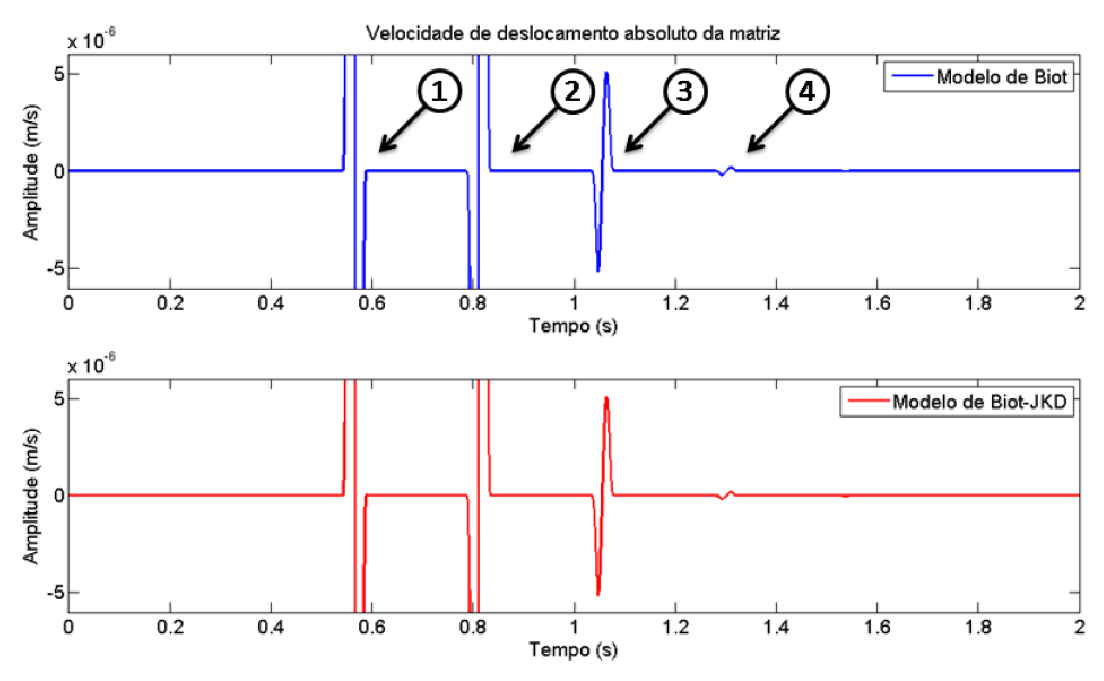
\includegraphics[scale=.65]{igor}
\caption{\textit{Velocidade de deslocamento da matriz para baixas frequ\^encias.}}
\label{fig.igor}
\end{figure}
Al\'em disso, no caso 1D a solu\c{c}\~ao do sistema de Biot pode ser formulada totalmente de maneira anal\'itica e expl\'icita. No caso 3D, todo o c\'odigo computacional s\'o pode ser implementado fazendo uso de opera\c{c}\~oes com matrizes, promovendo desafios em termos de aproxima\c{c}\~oes e instabilidades num\'ericas.


\section{Modelagem Matem\'atica e Num\'erica do Efeito Sismo-Magn\'etico}

Podemos observar uma an\'alise matem\'atica e num\'erica do efeito de indu\c{c}\~ao sismo-magn\'etica em \cite{mikhailenko_97}, onde \'e descrita a solu\c{c}\~ao simult\^anea de equa\c{c}\~oes el\'asticas com o acoplamento da for\c{c}a de Lorentz, e as equa\c{c}\~oes quasi-estacion\'arias de Maxwell com o acoplamento da velocidade de deslocamento do meio de propaga\c{c}\~ao das ondas. Tais sistemas de EDP's foram obtidos do modelo desenvolvido por \cite{Novacki_83} e foram transformados num sistema de EDO's utilizando transformadas finitas de Fourier.

O sistema de EDO's \'e escrito introduzindo uma matriz de vari\'aveis $A$, e a solu\c{c}\~ao num\'erica \'e obtida pelo m\'etodo de fatoriza\c{c}\~ao encontrado em \cite{Mikhailenko_89}, o qual utiliza a matriz de equa\c{c}\~oes de Riccati para a determina\c{c}\~ao das componentes $a_{ij}$. Tal abordagem n\~ao tem restri\c{c}\~oes computacionais se trabalhada com propaga\c{c}\~ao de ondas de alta frequ\^encia.

As simula\c{c}\~oes foram realizadas considerando ondas longitudinais, transversais e Rayleigh. Os resultados  mostraram, principalmente, que as primeiras chegadas das varia\c{c}\~oes geomagn\'eticas coincidiram com as chegadas dos tipos de ondas que as produziram. Essa coincid\^encia ocorreu para onda longitudinal, Rayleigh e para uma onda refletida na interface entre as camadas.









\chapter{Elementos da F\'isica-Matem\'atica}

\section{EDP de uma Onda}
Segundo \cite{farlow_93}, a EDP de uma onda 
\begin{equation}\label{eq.edp_geral}
\frac{\partial^2\mathbf{f}(\mathbf{x},t)}{\partial\,t^2}=\norm{\mathbf{v}}^2\nabla^2\mathbf{f}(\mathbf{x},t)
\end{equation}
possui a solu\c{c}\~ao de D'Alembert
\begin{equation}
\mathbf{f}(\mathbf{x},t)=\mathbf{g}_1(\mathbf{x}-\mathbf{v}\,t)+\mathbf{g}_2(\mathbf{x}+\mathbf{v}\,t),
\end{equation}
onde $\mathbf{x}=(x,y,z)^\top$ representa o espa\c{c}o $\mathbb{R}^3$, $\mathbf{v}$ \'e a \textit{velocidade} de propaga\c{c}\~ao da onda, $(\mathbf{x}\pm\mathbf{v}\,t)$ \'e a \textit{fase} da onda, $\mathbf{g}_1$ \'e a propaga\c{c}\~ao da onda no semiespa\c{c}o positivo do eixo $x$ e $\mathbf{g}_2$ \'e a propaga\c{c}\~ao da onda no semiespa\c{c}o negativo do eixo $x$.

De acordo com \cite{chew}, ondas tridimensionais oriundas de fonte pontual se propagam em formato esferoidal mas localmente podem ser tratadas como ondas planas, principalmente para raios distantes da fonte. A onda esf\'erica, solu\c{c}\~ao da EDP \ref{eq.edp_geral}, pode ser representada pela superposi\c{c}\~ao de ondas planas atrav\'es da identidade de \textit{Weyl}, onde tal superposi\c{c}\~ao tamb\'em \'e solu\c{c}\~ao da EDP \ref{eq.edp_geral}, conforme \cite{weyl_19}.

No $\mathbb{R}^3$ o \textit{vetor de onda} $\mathbf{k}=(k_x,k_y,k_z)^\top$ \'e aquele que aponta na dire\c{c}\~ao de propaga\c{c}\~ao da onda e sua magnitude, denominada \textit{n\'umero de onda}, \'e definida como 
\begin{equation}
\norm{\mathbf{k}}=k=\frac{\omega}{\norm{\mathbf{v}}},
\end{equation}
onde $\omega$ \'e a frequ\^encia temporal. Desta forma, a fase da onda pode ser escrita em termos do vetor de onda e da frequ\^encia como $(\mathbf{k}\cdot\mathbf{x}-\omega\,t)$, e a solu\c{c}\~ao da equa\c{c}\~ao \ref{eq.edp_geral} pode ser reescrita como uma superposi\c{c}\~ao de ondas planas
\begin{equation}
\mathbf{f}(\mathbf{x},t)=\mathbf{A}\,\sum_{\mathbf{k},\omega}{e^{i\,(\mathbf{k}\cdot\mathbf{x}-\omega\,t)}},
\end{equation}
onde $\mathbf{A}$ \'e a \textit{amplitude} da onda.

Podemos verificar em \cite{White_Zhou_2006}, para o caso $\mathbb{R}^2$ o \textit{vetor de onda horizontal} \'e definido como $\mathbf{k}=(k_x,k_y)^\top$, o \textit{n\'umero de onda horizontal} e a \textit{vagarosidade horizontal} s\~ao, respectivamente,
\begin{equation}\label{eq.numero_onda_vagarozidade_horizontal}
k=\sqrt{k_x^2+k_y^2}\qquad\text{e}\qquad\gamma=\frac{k}{\omega}.
\end{equation}
A vagarosidade vertical \'e definida como
\begin{equation}
q_0=\frac{1}{v_z},
\end{equation}
onde $v_z$ \'e a componente vertical da velocidade. Denotando o \textit{n\'umero de onda vertical} por $k_z$, temos que a \textit{vagarosidade vertical} pode ser escrita como
\begin{equation}
q_0=\frac{k_z}{\omega}.
\end{equation}
Combinando as vagarosidades horizontal e vertical, temos
\begin{equation}\label{eq.vagarosidade_vertical}
\gamma^2+q_0^2=\frac{1}{\norm{\mathbf{v}}^2}\qquad\text{ou}\qquad q_0=\sqrt{\epsilon_0\mu_0-\gamma^2},
\end{equation}
j\'a que $\epsilon_0\mu_0=\frac{1}{\norm{\mathbf{v}}^2}$.

\section{Transformadas Laterais de Fourier}

Segundo \cite{butkov_88}, podemos definir as transformadas laterais de Fourier direta e inversa entre o espa\c{c}o bidimensional e o vetor de onda horizontal como
\begin{align}\label{eq.trans_fourier_1}
\mathbf{\widehat{f}}(k_x,k_y,z) &= \iint_{\mathbb{R}^2}\mathbf{f}(x,y,z)\,e^{-i(k_xx+k_yy)}dx\,dy\\\nonumber\\\label{eq.trans_fourier_2}
\mathbf{f}(x,y,z) &= \left(\frac{1}{2\,\pi}\right)^2\iint_{\mathbb{R}^2}\mathbf{\widehat{f}}(k_x,k_y,z)\,e^{i(k_xx+k_yy)}dk_xdk_y.
\end{align}
O s\'imbolo $\,\widehat{}\,$ denota a fun\c{c}\~ao no espa\c{c}o da transformada lateral de Fourier.

A propriedade da transformada de derivadas \'e a que mais nos interessa e, supondo $f$ uma fun\c{c}\~ao escalar de uma \'unica vari\'avel, essa propriedade pode ser descrita como  
\begin{align*}
\widehat{f'}(x)&=\int_{-\infty}^{\infty}f'(x)\,e^{-i\,k_xx}dx\\
&=f(x)\,e^{-i\,k_xx}|_{-\infty}^{\infty}-(-i\,k_x)\int_{-\infty}^{\infty}f(x)\,e^{-i\,k_xx}dx\\
&=i\,k_x\widehat{f}(k_x).
\end{align*}
Na passagem da segunda para a terceira igualdade utilizamos a hip\'otese bastante difundida em geof\'isica de que $f(x)\rightarrow 0$ quando $x \rightarrow \pm \infty $, a qual podemos observar em demonstra\c{c}\~oes de teoremas como, por exemplo, o toerema de \textit{Helmholtz} encontrado em \cite{griffiths}. 


\section{Rota\c{c}\~oes}

Segundo \cite{lang_1986}, podemos produzir uma rota\c{c}\~ao antihor\'aria em torno do eixo $z$ aplicando o operador linear
\begin{equation*}
\begin{pmatrix}
\cos\theta&-\sin\theta&0\\
\sin\theta&\cos\theta&0\\
0&0&1
\end{pmatrix},
\end{equation*}
onde $\theta$ \'e o \^angulo que um vetor est\'a sendo rotacionado. Como a geometria do nosso problema considera ondas se propagando na parte negativa do eixo $z$ (consideramos $z$ positivo no sentido descendente), para produzirmos uma rota\c{c}\~ao antihor\'aria devemos considerar o \^angulo $-\theta$, e com isso nossa matriz de rota\c{c}\~ao se torna
\begin{equation*}
\begin{pmatrix}
\cos\theta&\sin\theta&0\\
-\sin\theta&\cos\theta&0\\
0&0&1
\end{pmatrix},
\end{equation*}
lembrando a paridade das fun\c{c}\~oes seno e cosseno. Para promovermos uma rota\c{c}\~ao orientando a primeira coordenada  no sentido de propaga\c{c}\~ao das ondas horizontais, temos que $\theta$ ser\'a o \^angulo entre $(x,0,0)^\top$ e $(k_x,k_y,0)^\top$, e a matriz de rota\c{c}\~ao se torna
\begin{equation}\label{eq.operador_rotacao}
\Omega=
\begin{pmatrix}
\frac{k_x}{k}&\frac{k_y}{k}&0\\
-\frac{k_y}{k}&\frac{k_x}{k}&0\\
0&0&1
\end{pmatrix}.
\end{equation}
Para escrevermos novamente as equa\c{c}\~oes no sistema de coordenadas original, precisamos aplicar a rota\c{c}\~ao inversa. Para isso, basta inverter a matriz de rota\c{c}\~ao \ref{eq.operador_rotacao} mas, como se trata de uma matriz ortogonal, a inversa \'e a sua transposta. Assim, usaremos
\begin{equation}\label{eq.rotacao_inversa}
\Omega^\top=
\begin{pmatrix}
\frac{k_x}{k}&-\frac{k_y}{k}&0\\
\frac{k_y}{k}&\frac{k_x}{k}&0\\
0&0&1
\end{pmatrix}.
\end{equation}


A rota\c{c}\~ao de um tensor $\tau$ \'e dada por 
\begin{equation}\label{eq.rotacao_tensor}
\tilde{\tau}=\Omega\,\tau\,\Omega^\top,
\end{equation}
e sua rota\c{c}\~ao inversa \'e dada por
\begin{equation}\label{eq.rot_inver_tensor}
\tau=\Omega^\top\tilde{\tau}\,\Omega.
\end{equation}


\section{A fun\c{c}\~ao $\delta$ de Dirac}\label{sec.dirac}

Em algumas aplica\c{c}\~oes f\'isicas pode ser necess\'ario trabalhar com conceito de um pulso de dura\c{c}\~ao infinitamente curta. De acordo com \cite{butkov_88}, podemos tomar o exemplo de um corpo colocado em movimento, a partir do repouso, atrav\'es de um golpe instant\^aneo que faz o mesmo adquirir um momento igual \`a impuls\~ao $I$ do choque, ou seja,
\begin{equation}
I=\int_{t_0}^{t_0+\Delta\,t}f(t)dt,
\end{equation}
onde $f(t)$ \'e a for\c{c}a e $\Delta\,t$ \'e o tempo de a\c{c}\~ao da for\c{c}a. A implus\~ao \'e um n\'umero finito e sua altera\c{c}\~ao ocorre instantaneamente, pois $\Delta\,t$ \'e um n\'umero muito pequeno. Assim, temos que a for\c{c}a deveria ter valor infinito durante o golpe e nula nos outros instantes, conforme o gr\'afico da figura \ref{fig.dirac}.
\begin{figure}
\centering
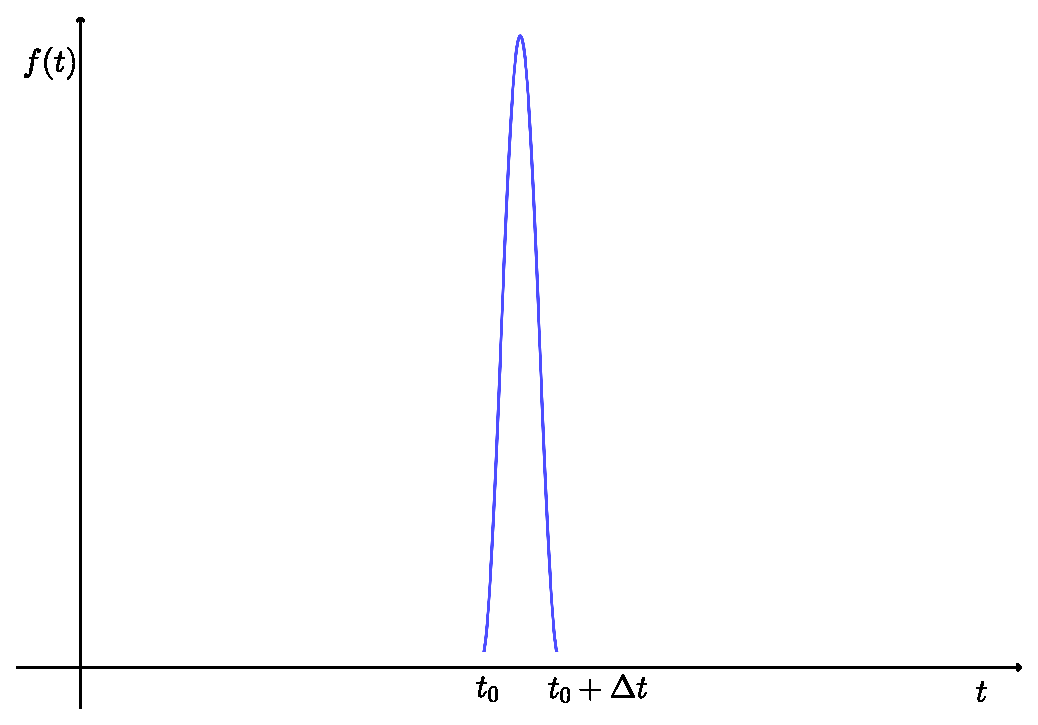
\includegraphics[scale=.6]{dirac_function}
\caption{\textit{Representa\c{c}\~ao de uma fun\c{c}\~ao fortemente concentrada.}}
\label{fig.dirac}
\end{figure}
A fim de facilitar v\'arias opera\c{c}\~oes da f\'isica-matem\'atica, Dirac prop\^os a introdu\c{c}\~ao da chamada fun\c{c}\~ao $\delta(x)$, que pode representar uma fun\c{c}\~ao infinitamente concentrada e \'e dada simbolicamente por
\begin{empheq}[left={\delta(x)=\empheqlbrace}]{align*}
0\,,&\quad\text{se}\quad x\neq 0\\
\infty\,,&\quad\text{se}\quad x=0
\end{empheq}
e $\delta$ deve satisfazer a seguinte condi\c{c}\~ao
\begin{equation}\label{eq.condicao_dirac}
\int_{-\infty}^{\infty}\delta(x)\,dx=1.
\end{equation}
Sendo $f$ uma fun\c{c}\~ao cont\'inua qualquer, a utilidade da fun\c{c}\~ao $\delta$ consiste em determinar o valor de 
\begin{equation}
\int_{-\infty}^{\infty}\delta(x)\,f(x)\,dx
\end{equation}
substituindo os limites de integra\c{c}\~ao por $-\epsilon$ e $\epsilon$, onde $\epsilon$ \'e um n\'umero positivo infinitesimalmente pr\'oximo de zero. Tal substitui\c{c}\~ao se justifica pois $\delta=0$ se $x\neq0$ e teremos uma aproxima\c{c}\~ao para o valor dessa integral. Assim, usando a defini\c{c}\~ao de $\delta$, a condi\c{c}\~ao \ref{eq.condicao_dirac} e a continuidade de $f$, temos
\begin{align*}
\int_{-\infty}^{\infty}\delta(x)\,f(x)\,dx&=\int_{-\infty}^{-\epsilon}\delta(x)\,f(x)\,dx+\int_{-\epsilon}^{\epsilon}\delta(x)\,f(x)\,dx+\int_{\epsilon}^{\infty}\delta(x)\,f(x)\,dx\\
&=\int_{-\epsilon}^{\epsilon}\delta(x)\,f(x)\,dx\\
&\approx\,f(0)\int_{-\epsilon}^{\epsilon}\delta(x)\,dx\\
&=f(0).
\end{align*}
Desta forma podemos representar a aplica\c{c}\~ao de uma fun\c{c}\~ao fortemente concentrada, incluindo a representa\c{c}\~ao de uma fonte pontual de onda s\'ismica que \'e de interesse geof\'isico, como veremos na subse\c{c}\~ao \ref{sec.presenca_fonte}.

\section{Fun\c{c}\~ao de Bessel de Primeira Esp\'ecie}

De acordo com \cite{butkov_88}, sendo $f(x)$ uma fun\c{c}\~ao qualquer, podemos escrever a equa\c{c}\~ao diferencial ordin\'aria de Bessel na forma
\begin{equation}
\frac{d^2f}{dx}+\frac{1}{x}\frac{df}{dx}+\left(1-\frac{m^2}{x^2} \right)\,f=0,
\end{equation}
onde, estudando o caso geral temos que $m$ \'e um n\'umero real arbitr\'ario que pode ser considerado n\~ao-negativo, mas no nosso trabalho vamos considerar $m$ inteiro positivo. A equa\c{c}\~ao acima \'e a EDO de Bessel de ordem $m$, suas solu\c{c}\~oes s\~ao conhecidas como fun\c{c}\~oes cil\'indricas e entre elas est\~ao as fun\c{c}\~oes de Bessel. Expandindo a fun\c{c}\~ao $f(x)$ numa s\'erie de \textit{Frobenius} e substituindo-a  na EDO de Bessel podemos deduzir que a solu\c{c}ao \'e dada por
\begin{equation}\label{eq.funcao_bessel_1}
J_m(x)=\sum_{j=0}^{\infty}(-1)^j\frac{x^{m+2\,j}}{j!\,\Gamma\,(m+j+1)\,2^{m+2\,j}}.
\end{equation}
A fun\c{c}\~ao $\Gamma$ \'e uma fun\c{c}\~ao fatorial de vari\'avel real com representa\c{c}\~ao na forma integral dada por
\begin{equation*}
\Gamma(\xi)=\int_0^\infty t^{\xi-1}e^tdt,\qquad x>0.
\end{equation*}
Como estamos trabalhando com $m$ inteiro positivo, a fun\c{c}\~ao $\Gamma(\xi)$ \'e dada simplesmente por $(\xi-1)!$. Assim, a express\~ao \ref{eq.funcao_bessel_1} passa a ser escrita como
\begin{equation}\label{eq.funcao_bessel_2}
J_m(x)=\sum_{j=0}^{\infty}\frac{(-1)^j}{j!\,(m+j)!}\left(\frac{x}{2}\right)^{m+2\,j}
\end{equation}
e \'e chamada fun\c{c}\~ao de Bessel de primeira esp\'ecie de ordem $m$.

\section{Transformadas de Hankel}\label{sec.trans_hankel}
A transformada de Hankel utiliza as fun\c{c}\~oes de Bessel para transformar um sistema de coordenadas $\mathbf{x}$ para outro $\pmb{\xi}$. De acordo com \cite{baruch_2013}, assumindo que $f$ seja uma fun\c{c}\~ao radial, ou seja, que depende apenas da magnitude $x$ de $\mathbf{x}$, umas das defini\c{c}\~oes da transformada de Hankel \'e dada por
\begin{equation*}
\mathcal{B}_m[f(x)](\xi)=\int_0^\infty x\,J_m(x\,\xi)\,f(x)\,dx.
\end{equation*}
E a transformada inversa, considerando $\xi=\norm{\pmb{\xi}}$, \'e
\begin{equation*}
\mathcal{B}^{-1}_m[F(\xi)](x)=\int_0^\infty \xi\,J_m(x\,\xi)\,F(\xi)\,d\xi,
\end{equation*}
onde $J_m$ \'e uma fun\c{c}\~ao de Bessel de primeira esp\'ecie de ordem $m$, conforme visto na subse\c{c}\~ao anterior.











\chapter{Fundamentos de eletromagnetismo}\label{sec.fund_eletr}

\section{Introdução}

\section{Fatos experimentais}

\subsection{Lei de Gauss para os fluxos elétrico e magnético}
De acordo com \cite{jackson_classical_1999} e \cite{sommerfeld_52} , os conceitos, definições e resultados em eletromagnetismo clássico partem das experiências de Cavendish e Coulomb no final do Séc. $XVIII$. A partir desses experimentos foi estabelecida a Lei de Coulomb
\begin{equation}\label{eq.forc_elet}
\textbf{F}=k\,\frac{q_1\,q_2}{||\textbf{x}_1-\textbf{x}_2||^2}\frac{\textbf{x}_1-\textbf{x}_2}{||\textbf{x}_1-\textbf{x}_2||},
\end{equation}
onde $q_i$ são as cargas elétricas (campos escalares) presentes nos pontos $\textbf{x}_i$, respectivamente, $k$ (campo escalar) é uma constante de proporcionalidade cujo valor depende do sistema de unidades de medida adotado, $||\textbf{x}_1-\textbf{x}_2||^2$ é a distância euclidiana entre as cargas e $\textbf{F}$ é a força elétrica exercida pela carga $q_1$ sobre a carga $q_2$. As notações em negrito representam campos vetorias pertencentes ao espaço $\mathbb{R}^3$, e o vetor normal que fornece a direção de interação entre as cargas é dado por $(\textbf{x}_1-\textbf{x}_2)/||\textbf{x}_1-\textbf{x}_2||$.

O campo elétrico $\textbf{E}$ é definido como sendo a força elétrica por unidade de carga em um determinado ponto que contém a carga de prova $q_2$, portanto é uma função vetorial que depende da posição da carga de prova em relação à carga fonte $q_1$, ou seja,
\begin{equation}\label{eq.camp_elet}
\textbf{E}=\lim_{q_2\to 0}\frac{\textbf{F}}{q_2}.
\end{equation}
A carga de prova foi tomada infinitesimalmente pequena para que o campo gerado por ela não perturbe a carga fonte. Experimentalmente, tanto a direção da força como a razão entre a força e a quantidade de carga vão se tornando constantes à medida que a quantidade de carga se torna cada vez menor, definindo a magnitude e a direção do campo elétrico. No SI, a unidade de medida de carga é o \textit{coulomb} $(C)$, o campo elétrico é o \textit{newton/coulomb} $(N/C)$ ou o \textit{volt/metro} $(V/m)$, e a constante $k=(4\pi\,\epsilon_0)^{-1}$ onde $\epsilon_0\simeq8.854\times10^{-12}$ é a permissividade elétrica no vácuo medida em \textit{farad/m} $(F/m)$.

Substituindo a equação \ref{eq.camp_elet} em \ref{eq.forc_elet} temos que o campo elétrico agindo num ponto $\textbf{x}$ qualquer devido a uma carga $q_1$ no ponto $\textbf{x}_1$ é
\begin{equation}\label{eq.campo_eletrico}
\textbf{E}=k\,\frac{q_1}{||\textbf{x}_1-\textbf{x}||^2}\frac{\textbf{x}_1-\textbf{x}}{||\textbf{x}_1-\textbf{x}||},
\end{equation}
como podemos observar na figura \ref{fig.camp_eletr} simulando um sistema de coordenadas qualquer.
\begin{figure}[!htb]
\centering
\includegraphics[scale=1.5]{camp_elet}
\caption{\textit{Exemplificação da interação entre cargas elétricas devido à geração, em função de $q_1$, de um campo elétrico. A força elétrica $\textbf{F}$ atuando numa carga qualquer $q$ tem mesma direção do campo elétrico $\textbf{E}$, com mesmo sentido ou sentido oposto conforme a carga $q$ é positiva ou negativa, respectivamente.}}
\label{fig.camp_eletr}
\end{figure}

%\begin{figure}[!htb]
%\centering
%\subfloat{\includegraphics[scale=1]{camp_elet_3D}}
%\subfloat{\includegraphics[scale=1]{camp_elet_3D2}}
%\caption{}
%\label{fig.mossul}
%\end{figure}

Num sistema com mais de uma carga fonte produzindo campos elétricos, foi observado experimentalmente que o campo elétrico total atuando num ponto $\textbf{x}$ é simplesmente o somatório dos campos produzidos por cada carga, o que ficou conhecido como a \textit{Superposição Linear} e pode ser expressada na forma
\begin{equation*}
\textbf{E}=k\,\sum_{i=1}^{n}q_i\,\frac{\textbf{x}_i-\textbf{x}}{||\textbf{x}_i-\textbf{x}||^3}.
\end{equation*} 
O campo elétrico devido a um pequeno número de cargas pode ser calculado a partir do princípio da superposição linear. Mas se temos uma quantidade muito grande de cargas num determinado volume $V$, devemos calcular a \textit{densidade volumétrica de carga} $\rho$ num volume infinitesimal situado em $\textbf{x}_0$ e em seguida integrar sobre o volume $V$ para obter a quantidade total de carga $Q$. A densidade de carga é definida por
\begin{equation*}
\rho(\textbf{x}_0)=\lim_{\Delta V_i \to 0}\frac{\Delta q_i}{\Delta V_i}=\frac{d\,q}{d\,V},
\end{equation*}
medida, no SI, em $C/m^3$. A quantidade total de carga $Q=\sum_i \Delta\,q_i$ no volume $V$ é
\begin{equation*}
Q=\int_{V}\rho(\textbf{x}_0)\,dV.
\end{equation*}

O \textit{fluxo elétrico} é definido como a quantidade linhas do campo elétrico que atravessa uma dada superfície, e é dado pela equação
\begin{equation*}
\Phi_\textbf{E}=\textbf{E}\cdot\textbf{A}. 
\end{equation*} 
O \textit{vetor área} é definido como a magnitude da área da superfície atravessada apontando na direção do vetor normal, $\textbf{A}=A\,\textbf{n}$, e estamos considerando um campo elétrico uniforme $\textbf{E}$ que se desloca na direção $\textbf{n}$, ou seja, é perpendicular à superfície $A$ como podemos observar na figura \ref{fig.flux_ele}.
\begin{figure}[!htb]
\centering
\includegraphics[scale=.5]{campo_area}
\caption{\textit{Fluxo elétrico, linhas de campo elétrico passando através de uma superfície.}}
\label{fig.flux_ele}
\end{figure}
Mas se o campo elétrico se propaga formando um ângulo $\theta$ com o vetor normal da superfície, então o fluxo elétrico é dado por
\begin{equation*}
\Phi_\textbf{E}=\textbf{E}\cdot\textbf{A}=E\,A\,\cos\theta,
\end{equation*}
com $E=\textbf{E}\cdot\textbf{n}$ sendo a componente do campo elétrico na direção $\textbf{n}$. Em geral uma superfície pode ser curva e estamos interessados numa superfície \textit{fechada}, ou seja, aquela que engloba um determinado volume, o qual contém uma carga elétrica. Tomando uma área bem pequena dessa superfície, $\Delta\textbf{A}_i$, o campo elétrico pode ser variável em cada parte da superfície e nessas condições temos que o fluxo nessa pequena região é dado por
\begin{equation*}
\Delta\,\Phi_\textbf{E}=\textbf{E}_i\cdot\Delta\,\textbf{A}_i.
\end{equation*}
O fluxo positivo atravessando toda a superfície de dentro para fora é calculado tomando o limite quando $\Delta\textbf{A}_i\to 0$ e aumentando infinitamente a quantidade dessas pequenas áreas
\begin{equation}\label{eq.fluxo_eletr}
\Phi_\textbf{E}=\lim_{i\to\infty}\sum_i\textbf{E}_i\cdot\textit{d}\textbf{A}_i=\int\int_S\textbf{E}\cdot\textit{d}\textbf{A}.
\end{equation}

Considere uma carga pontual positiva $q$ localizada no centro de uma esfera imaginária de raio $r$, onde essa carga produz um campo elétrico que aponta na direção radial conforme a figura \ref{fig.esfe_gauss}. Sabemos que a área da superfície dessa esfera é dada por $A=4\pi\,r^2$ e que, segundo a equação \ref{eq.campo_eletrico}, a magnitude do campo elétrico em qualquer ponto da superfície esférica é
\begin{equation*}
E=\frac{q}{4\pi\epsilon_0\,r^2},
\end{equation*}
assim o fluxo elétrico é calculado usando a equação \ref{eq.fluxo_eletr}.
\begin{align*}
\Phi_\textbf{E}&=\int\int_S\textbf{E}\cdot\textit{d}\textbf{A}\\
&=\int\int_S\textbf{E}\cdot\textbf{n}\,\textit{d}A\\
&=E\,\int\int_S\textit{d}A\\
&=E\,A\\
&=\frac{q}{4\pi\epsilon_0\,r^2}\,4\pi\,r^2\\
&=\frac{q}{\epsilon_0}.
\end{align*}
Na demonstração acima escolhemos uma esfera como \textit{superfície Gaussiana} mas, introduzindo o conceito de \textit{ângulo sólido}, vemos que a demonstração é válida para qualquer superfície fechada, utilizada em aplicações que apresentem mais ou menos alguma simetria (esférica, planar ou cilíndrica). Para mais detalhes consultar \cite{jackson_classical_1999}. Assim, concluímos que o fluxo elétrico através de uma superfície fechada que apresente mais ou menos alguma simetria é diretamente proporcional à quantidade de carga enclausurada pela superfície. Matematicamente, a \textit{lei de Gauss} para o fluxo elétrico é
\begin{equation*}
\Phi_\textbf{E}=\int\int_S\textbf{E}\cdot\textit{d}\textbf{A}=\frac{q}{\epsilon_0}.
\end{equation*}
\begin{figure}[!htb]
\centering
\includegraphics[scale=.6]{esfera_gaussiana}
\caption{\textit{Esfera Gaussiana enclausurando uma carga positiva $q$. Nessas condições, o ângulo entre o vetor campo elétrico e o vetor normal à superfície infinitesimal $d\textbf{A}$ é zero.}}
\label{fig.esfe_gauss}
\end{figure}

Uma carga elétrica produz um campo elétrico, e de maneira similar uma barra magnética, ou ímã, produz um \textit{campo magnético} $\textbf{B}$. Um ímã possui um polo norte de onde partem as linhas de campo magnético e um polo sul por onde as linhas de campo magnético retornam ao ímã (figura \ref{fig.barras_mag}). Diferentemente das cargas elétricas que são observadas isoldamente na natureza, os dois polos magnéticos sempre aparecem aos pares, ou seja, monopolos magnéticos não existem isoladamente apesar de a suposição de sua existência ser de interesse teórico. Assim, sempre que um ímã é fracionado, mesmo que em partes muito elementares, o resultado sempre será um novo ímã com dois polos magnéticos conforme a figura \ref{fig.barras_mag}.
\begin{figure}[!htb]
\centering
\includegraphics[scale=.7]{barras_magn}
\caption{\textit{Barras magnéticas onde polos de mesmo sinal se repelem e polos de sinais contrários se atraem.}}
\label{fig.barras_mag}
\end{figure}
Como não existem monopolos magnéticos, o campo magnético deve ser definido de forma diferente do campo elétrico, e experimentalmente foram observadas algumas características relacionadas ao movimento de uma carga elétrica $q$ com velocidade $\textbf{v}$ num campo magnético $\textbf{B}$:
\begin{itemize}
\item a magnitude da força magnética $\textbf{F}_B$ é proporcional à $v$, $B$ e $q$, onde $v$ e $B$ são as magnitudes da velocidade e do campo magnético respectivamente,
\item a direção de $\textbf{F}_B$ é perpendicular ao plano formado por $\textbf{v}$ e $\textbf{B}$,
\item $\textbf{F}_B$ é proporcional ao $\sin\theta$, o ângulo formado por $\textbf{v}$ e $\textbf{B}$. Se $\textbf{v}$ e $\textbf{B}$ são paralelos então $\textbf{F}_B=0$, e
\item o sentido de $\textbf{F}_B$ depende do sinal da carga $q$.
\end{itemize}
Essas observações são ilustradas na figura \ref{fig.froca_mag_veloc} e a força magnética é definida como
\begin{equation*}
\textbf{F}_B=q\textbf{v}\times\textbf{B}.
\end{equation*}
\begin{figure}[!htb]
\centering
\includegraphics[scale=.5]{forca_camp_mag_veloc}
\caption{\textit{Força magnética agindo numa carga elétrica que se desloca num campo magnético.}}
\label{fig.froca_mag_veloc}
\end{figure}
Teoricamente, poderíamos tentar determinar a lei de Gauss para o fluxo magnético com o mesmo procedimento aplicado ao fluxo elétrico e obter
\begin{equation*}
\Phi_\textbf{B}=\int\int_S\textbf{B}\cdot\textit{d}\textbf{A}=\frac{q_m}{\mu_0},
\end{equation*} 
onde $q_m$ é a carga magnética (suposto monopolo magnético) enclausurado pela superfície Gaussiana, $B$ é o campo magnético e $\mu_0$ é a \textit{permeabilidade magnética no vácuo}. No entanto, não foi constatada a existência de qualquer carga magnética isolada mesmo após muitos esforços. Como $q_m=0$, temos que a lei de Gauss para o magnetismo é
\begin{equation}\label{eq.gauss_flux_mag}
\Phi_\textbf{B}=\int\int_S\textbf{B}\cdot\textit{d}\textbf{A}=0.
\end{equation}
Conforme podemos ver na figura tal, a equação \ref{eq.gauss_flux_mag} implica que a quantidade de linhas do campo magnético saindo da superfície é igual à quantidade que está entrando, ou seja, não há uma origem isolada e um término isolado para o fluxo magnético como há para o fluxo elétrico. Outro problema é que a barra imantada atravessa a superfície que, de acordo com a hipóteses da lei de Gauss, deveria ser fechada.
\begin{figure}[!htb]
\centering
\includegraphics[scale=.3]{flux_ele_mag}
\caption{\textit{As linhas do campo magnético que emanam do polo norte do ímã em direção ao polo sul retornam para dentro da superfície Gaussiana descrevendo um laço fechado.}}
\label{fig.flux_elet_magn}
\end{figure}




\section{Equações de Maxwell}

\section{Generalizações da teoria}

\section{Conclusões}
\chapter{Fundamentos de Elasticidade}\label{sec.fund_elast}

\section{Introdu\c{c}\~ao}
A teoria formal da propaga\c{c}\~ao de ondas s\'ismicas repousa nas intera\c{c}\~oes entre as particulas infinitesimais discretas do meio \`a medida que uma deforma\c{c}\~ao se propaga. \'E muito dif\'icil estudar individualmente cada uma dessas intera\c{c}\~oes, mas dados experimentais que foram coletados como resultados dessas intera\c{c}\~oes sugerem que as mesmas podem ser consideradas em conjunto. Assim, o estudo da propaga\c{c}\~ao de ondas s\'ismicas atrav\'es de camadas de subsuperf\'icie num material discretizado pode ser feito considerando o meio como cont\'inuo, e tais estudos s\~ao os objetos da \textit{mec\^anica do cont\'inuo}. 

No desenvolvimento te\'orico da mec\^anica do cont\'inuo nao s\~ao consideradas as caracter\'isticas at\^omicas da mat\'eria bem como as intera\c{c}\~oes entre essas part~\'iculas, ou seja, a mat\'eria n\~ao \'e estudada do ponto de vista microsc\'opico. Segundo \cite{slawinski}, tal abordagem se justifica pelo fato de que a mat\'eria \'e formada por part\'iculas suficientemente pouco espa\c{c}adas e suas caracter\'isticas e comportamento podem ser descritos por fun\c{c}\~oes cont\'inuas e diferenci\'aveis. Assim, \'e assummido que elementos infinitesimais da mat\'eria t\^em as mesmas propriedades observadas em experimentos macrosc\'opicos, pois essa hip\'otese permite a cria\c{c}\~ao de um modelo matem\'atico abstrato \textit{efetivo} na descri\c{c}\~ao da realidade f\'isica. Como exemplo, vamos considerar a cor de um objeto. Pr\'otons e el\'etrons n\~ao possuem cor, mas os meios materiais (que s\~ao formados por pr\'otons e el\'etrons) t\^em a capacidade de absorver ou refletir determinados comprimentos de ondas eletromagn\'eticas as quais determinam a cor de cada meio. Outros conceitos da mec\^anica do cont\'inuo sao elasticidade, viscosidade, fric\c{c}\~ao, rigidez, etc, como veremos mais a frente.


\section{Fatos experimentais}
A teoria sobre elasticidade est\'a baseada em conceitos primitivos e conclus\~oes estabelecidas a partir de fatos experimentais verificados em v\'arios textos sobre o assunto como \cite{liu}, \cite{dahlem} e \cite{slawinski}. Adicionalmente, em geral as equa\c{c}\~oes que governam a propaga\c{c}\~ao de ondas em meios el\'asticos s\~ao n\~ao-lineares. Contudo, em experimentos s\'ismicos foi constatado que aspectos importantes da propaga\c{c}\~ao de ondas podem ser analisados a partir de equa\c{c}\~oes lineares, resultando numa abordagem chamada \textit{teoria da elasticidade linearizada}.

\subsection{Deforma\c{c}\~ao}

A \textit{deforma\c{c}\~ao} de um meio el\'astico cont\'inuo \'e a mudan\c{c}a na posi\c{c}\~ao dos pontos que comp\~oem o corpo em rela\c{c}\~ao uns aos outros. Ou seja, h\'a uma mudan\c{c}a relativa entre os pontos e n\~ao um deslocamento do corpo como um todo e sem mudan\c{c}a de sua forma, caso em que ter\'iamos um \textit{movimento r\'igido}. Nesta subse\c{c}\~ao estamos interessados nas caracter\'isticas geom\'etricas relativas a deforma\c{c}\~ao de um corpo. N\~ao estamos considerando as causas de deforma\c{c}\~ao de um corpo, como aplica\c{c}\~ao de carga ou varia\c{c}\~ao de temperatura, nem discutiremos a composi\c{c}\~ao do material, assumindo apenas que o mesmo seja cont\'inuo e el\'astico. Assim, vamos relacionar as caracter\'isticas geom\'etricas de um corpo antes da deforma\c{c}\~ao com as caracter\'isticas ap\'os a deforma\c{c}\~ao.

\subsection{Dedu\c{c}\~ao do Tensor de Deforma\c{c}\~oes}

Para determinar o tensor de deforma\c{c}\~oes vamos considerar dois pontos pertencentes ao espaco $\mathbb{R}^3$ bastante pr\'oximos um do outro denotados por
\begin{align*}
\mathbf{x}&=(x_1,x_2,x_3)\\
\mathbf{y}=\mathbf{x}+d\mathbf{s}&=(x_1+dx_1,x_2+dx_2,x_3+dx_3).
\end{align*}
O quadrado da dist\^ancia entre esses dois pontos \'e
\begin{equation}\label{eq.dist_antes_defor}
\norm{d\mathbf{s}}^2=(dx_1)^2+(dx_2)^2+(dx_3)^2.
\end{equation}
A aplica\c{c}\~ao de uma deforma\c{c}\~ao depende do ponto de aplica\c{c}\~ao, ou seja, a deforma\c{c}\~ao aplicada no ponto $\mathbf{x}$ difere da aplica\c{c}\~ao no ponto $\mathbf{y}$. Caso o vetor que d\'a a deforma\c{c}\~ao tenha componentes constantes, n\~ao teremos uma deforma\c{c}\~ao relativa, apenas um transla\c{c}\~ao dos pontos. Assim, podemos definir o \textit{vetor de deslocamento} para cada ponto de aplica\c{c}\~ao
\begin{align*}
\mathbf{u}&=(u_1,u_2,u_3)\\
\mathbf{v}&=(v_1,v_2,v_3),
\end{align*}
e som\'a-los aos respectivos pontos $\mathbf{x}$ e $\mathbf{y}$ para obter suas posi\c{c}\~oes ap\'os a deforma\c{c}\~ao,
\begin{align*}
\mathbf{x}^*&=(x_1+u_1,x_2+u_2,x_3+u_3)\\
\mathbf{y}^*&=(x_1+dx_1+v_1,x_2+dx_2+v_2,x_3+dx_3+v_3).
\end{align*}
Subtraindo, obtemos o vetor que d\'a a diferen\c{c}a entre os pontos ap\'os a deforma\c{c}\~ao
\begin{equation}\label{eq.dist_apos_defor}
d\mathbf{s}^*=(dx_1+v_1-u_1,dx_2+v_2-u_2,dx_3+v_3-u_3).
\end{equation}
Como a varia\c{c}\~ao entre os pontos $\mathbf{x}$ e $\mathbf{y}$ \'e infinitesimal, vamos aplicar a expans\~ao de Taylor de segunda ordem em torno do ponto $\mathbf{x}$ e desprezar o resto de Lagrange para escrever as componentes de $\mathbf{v}$ em fun\c{c}\~ao das componentes de $\mathbf{u}$, aproximadamente,
\begin{align*}
v_1&\approx u_1+\frac{\partial u_1}{\partial x_1}\Bigg\vert_{\mathbf{x}}dx_1+\frac{\partial u_1}{\partial x_2}\Bigg\vert_{\mathbf{x}}dx_2+\frac{\partial u_1}{\partial x_3}\Bigg\vert_{\mathbf{x}}dx_3\\\\
v_2&\approx u_2+\frac{\partial u_2}{\partial x_1}\Bigg\vert_{\mathbf{x}}dx_1+\frac{\partial u_2}{\partial x_2}\Bigg\vert_{\mathbf{x}}dx_2+\frac{\partial u_2}{\partial x_3}\Bigg\vert_{\mathbf{x}}dx_3\\\\
v_3&\approx u_3+\frac{\partial u_3}{\partial x_1}\Bigg\vert_{\mathbf{x}}dx_1+\frac{\partial u_3}{\partial x_2}\Bigg\vert_{\mathbf{x}}dx_2+\frac{\partial u_3}{\partial x_3}\Bigg\vert_{\mathbf{x}}dx_3.
\end{align*}
Substituindo esses valores na equa\c{c}\~ao \ref{eq.dist_apos_defor}, simplificando e introduzindo a nota\c{c}\~ao de somat\'orio temos
\begin{equation*}
d\mathbf{s}^*\approx\left(dx_1+\sum_{i=1}^3\frac{\partial u_1}{\partial x_i}\Bigg\vert_{\mathbf{x}}dx_i\,,\,dx_2+\sum_{i=1}^3\frac{\partial u_2}{\partial x_i}\Bigg\vert_{\mathbf{x}}dx_i\,,\,dx_3+\sum_{i=1}^3\frac{\partial u_3}{\partial x_i}\Bigg\vert_{\mathbf{x}}dx_i\right).
\end{equation*}
O quadrado da dist\^ancia entre os pontos ap\'os a deforma\c{c}\~ao \'e dado por
\begin{equation*}
\norm{d\mathbf{s}^*}^2\approx\left(dx_1+\sum_{i=1}^3\frac{\partial u_1}{\partial x_i}\Bigg\vert_{\mathbf{x}}dx_i\right)^2+\left(dx_2+\sum_{i=1}^3\frac{\partial u_2}{\partial x_i}\Bigg\vert_{\mathbf{x}}dx_i\right)^2+\left(dx_3+\sum_{i=1}^3\frac{\partial u_3}{\partial x_i}\Bigg\vert_{\mathbf{x}}dx_i\right)^2.
\end{equation*}
Abrindo cada uma das parcelas quadr\'aticas, temos
\begin{align*}
\norm{d\mathbf{s}^*}^2&\approx(dx_1)^2+2\,dx_1\,\sum_{i=1}^3\frac{\partial u_1}{\partial x_i}\Bigg\vert_{\mathbf{x}}dx_i+\left(\sum_{i=1}^3\frac{\partial u_1}{\partial x_i}\Bigg\vert_{\mathbf{x}}dx_i\right)^2\\\\
&+(dx_2)^2+2\,dx_2\,\sum_{i=1}^3\frac{\partial u_2}{\partial x_i}\Bigg\vert_{\mathbf{x}}dx_i+\left(\sum_{i=1}^3\frac{\partial u_2}{\partial x_i}\Bigg\vert_{\mathbf{x}}dx_i\right)^2\\\\
&+(dx_3)^2+2\,dx_3\,\sum_{i=1}^3\frac{\partial u_3}{\partial x_i}\Bigg\vert_{\mathbf{x}}dx_i+\left(\sum_{i=1}^3\frac{\partial u_3}{\partial x_i}\Bigg\vert_{\mathbf{x}}dx_i\right)^2.
\end{align*}
Pela equa\c{c}\~ao \ref{eq.dist_antes_defor}, a coluna  da esquerda \'e $\norm{d\mathbf{s}}^2$. Como estamos trabalhando com quantidades infinitesimais, podemos negligenciar a coluna da direita por se tratar do quadrado do gradiente de cada componente do vetor de deslocamento num produto escalar com o vetor que d\'a a dist\^ancia entre os pontos $\mathbf{x}$  e $\mathbf{y}$. Assim,
\begin{equation*}
\norm{d\mathbf{s}^*}^2\approx\norm{d\mathbf{s}}^2+\sum_{i=1}^3\sum_{j=1}^3\left(\frac{\partial u_i}{\partial x_j}\Bigg\vert_{\mathbf{x}}+\frac{\partial u_j}{\partial x_i}\Bigg\vert_{\mathbf{x}}\right)dx_i\,dx_j,
\end{equation*}
onde o termo entre par\^enteses \'e definido como o \textit{tensor de deforma\c{c}\~ao} na teoria da elasticidade,
\begin{equation*}
\varepsilon_{i,j}=\frac{1}{2}\left(\frac{\partial u_i}{\partial x_j}\Bigg\vert_{\mathbf{x}}+\frac{\partial u_j}{\partial x_i}\Bigg\vert_{\mathbf{x}}\right),\qquad\text{onde}\qquad i,j\,\in\,\{1,2,3\}.
\end{equation*}








\section{Equações de Lamé}

\section{Generalizações da teoria}

\section{Conclusões}
\chapter{Acoplamento Magneto-elástico}

\section{Introdução}

\section{Modelo de Dunkin e Erigen}

\section{Conclusões}
\chapter{Recondicionamento do Modelo de Dunkin e Erigen}\label{sec.recon_model_dun_eri}
Uma das contribui\c{c}\~oes dessa monografia \'e a utiliza\c{c}\~ao de hip\'oteses simplificadoras de ordem f\'isica e experimental, dispon\'iveis na literatura, para reeescrever o modelo do acoplamento magneto-el\'astico de forma que o mesmo possa receber um tratamento matem\'atico e computacional, no sentido de solucionar um problema direto.

Como vimos na subse\c{c}\~ao \ref{sec.magnetizacao_polarizacao}, a polariza\c{c}\~ao e magnetiza\c{c}\~ao de um determinado material depende das caracter\'isticas de cada material. De acordo com \cite{jackson_classical_1999} e \cite{griffiths}, as equa\c{c}\~oes constitutivas apresentadas na subse\c{c}\~ao \ref{sec.constitutivas_dunkin} podem n\~ao ser simples pois existe uma diversidade enorme de propriedades el\'etricas e magn\'eticas dos materias, especialmente em s\'olidos cristal\'inicos  e materias ferroel\'etricos e ferromagn\'eticos que t\^em polariza\c{c}\~ao e magnetiza\c{c}\~ao n\~ao nulos mesmo na absten\c{c}\~ao de aplica\c{c}\~ao de campos eletromagn\'eticos. Com excess\~ao desses tipos de materias, a aplica\c{c}\~ao de campos eletromagn\'eticos produzem polariza\c{c}\~ao e magnatiza\c{c}\~ao proporcional aos campos aplicados, e a rela\c{c}\~ao do campo de densidade de fluxo el\'etrico com o campo el\'etrico bem como a rela\c{c}\~ao do campo magn\'etico auxiliar com o campo magn\'etico s\~ao consideradas lineares, pois a contribui\c{c}\~ao das parcelas n\~ao-lineares tornam-se desprez\'iveis. Podemos ainda considerar a permeabilidade magn\'etica de muitos materiais tendo valor muito pr\'oximo da permeabilidade magn\'etica no v\'acuo, assim $\mu=\mu_0$. Com isso, temos que o escalar $\alpha$ definido em \ref{eq.constitutiva_1} tem seu valor considerado nulo, e as express\~oes para o campo de densidade de fluxo el\'etrico e o campo magn\'etico da subse\c{c}\~ao \ref{sec.constitutivas_dunkin} se tornam
\begin{align}\label{eq.constitutiva_alpha_1}
\mathbf{D}&=\epsilon\,\mathbf{E}\\\nonumber\\\label{eq.constitutiva_alpha_2}
\mathbf{B}&=\mu\,\mathbf{H}.
\end{align}
Substituindo a equa\c{c}\~ao \ref{eq.constitutiva_alpha_1} na equa\c{c}\~ao \ref{eq.campo_dunkin_1} e aplicando a transformada de Fourier, temos a rela\c{c}\~ao entre o campo el\'etrico e o campo magn\'etico auxiliar dada por
\begin{equation}
\nabla\times\mathbf{\widehat{E}}=i\,\omega\,\mu_0\mathbf{\widehat{H}},
\end{equation}
onde $i$ \'e um n\'umero complexo, $\omega$ \'e a frequ\^encia temporal e a nota\c{c}\~ao $\widehat{\,\,}$ significa que a fun\c{c}\~ao vetorial est\'a no dom\'inio da frequ\^encia temporal.

Ondas eletromagn\'eticas se propagam com velocidade da luz que \'e limitada. Segundo \cite{jackson_classical_1999}, num sistema onde as dimens\~oes s\~ao pequenas comparadas ao comprimento de onda eletromagn\'etica e comparadas \`a escala de tempo dominante, podemos tratar a velocidade da luz como instant\^anea num regime denominado \textit{quasi-estacion\'ario}. Como consequ\^encia dessa premissa, em meios condutivos a contribui\c{c}\~ao do campo de densidade de fluxo el\'etrico \'e muito pequena quando comparada \`a contribui\c{c}\~ao da densidade de corrente el\'etrica na produ\c{c}\~ao de campos magn\'eticos. Assim, podemos desprezar a parcela referente \`a corrente deslocada introduzida por Maxwell na lei de Amper\`e, o que implica (pela equa\c{c}\~ao \ref{eq.campo_dunkin_3}) em $\rho_e=0$. 
Vamos supor ainda que o campo magn\'etico auxiliar medido durante o efeito magneto-el\'astico seja uma combina\c{c}\~ao do campo magn\'etico gerado $\mathbf{H}$ mais o campo magn\'etico natural da Terra $\mathbf{H}^0$, e para manter a nota\c{c}\~ao vamos usar a substitui\c{c}\~ao 
\begin{equation}
\mathbf{H}\longrightarrow\mathbf{H}+\mathbf{H}^0.
\end{equation}
Utilizando a equa\c{c}\~ao \ref{eq.constitutiva_alpha_2}, o campo de densidade de corrente el\'etrica dado pela subse\c{c}\~ao \ref{sec.constitutivas_dunkin} poder ser reescrito como
\begin{equation}
\mathbf{J}=\sigma\,\mathbf{E}+\mathbf{v}\times\sigma\,\mu_0\mathbf{H}.
\end{equation}
Substituindo esta \'ultima rela\c{c}\~ao juntamente com a equa\c{c}\~ao \ref{eq.constitutiva_alpha_1} na equa\c{c}\~ao \ref{eq.campo_dunkin_2}, e aplicando a transformada de Fourier, temos
\begin{equation}
\nabla\times\mathbf{\widehat{H}}=(\sigma-i\,\epsilon\,\omega)\,\mathbf{\widehat{E}}+\mathbf{\widehat{v}}\times\sigma\mu_0\mathbf{H}^0,
\end{equation}
onde $\mathbf{\widehat{v}}=-i\,\omega\mathbf{\widehat{u}}$ \'e a velocidade de deslocamento do meio. Na dedu\c{c}\~ao da equa\c{c}\~ao acima, estamos considerando que a contribui\c{c}\~ao da parcela $\mathbf{\widehat{v}}\times\sigma\mu_0\mathbf{\widehat{H}}$ \'e desprez\'ivel se comparada \`a contribui\c{c}\~ao do campo geomagn\'etico, ainda como uma consequ\^encia do regime quasi-estacion\'ario.

De acordo com \cite{Knopoff_1955}, a altera\c{c}\~ao que o campos eletromagn\'eticos aplicam em ondas el\'asticas \'e desprez\'ivel, e assim podemos excluir a for\c{c}a de Lorentz e reescrever a equa\c{c}\~ao \ref{eq.campo_dunkin_5} no dom\'inio da frequ\^encia na forma matricial como 
\begin{equation}
-i\,\omega\rho\,\mathbf{\widehat{v}}=\nabla\cdot\widehat{\tau} + \mathbf{\widehat{F}}.
\end{equation}
A lei de Hooke dada na subse\c{c}\~ao \ref{sec.constitutivas_dunkin} pode ser reescrita no dom\'inio da frequ\^encia e em sua forma matricial como
\begin{equation}
\widehat{\tau}=\lambda\,\nabla\cdot\mathbf{\widehat{u}}\cdot\,I + \mu\,(\nabla\,\mathbf{\widehat{u}}+\nabla\mathbf{\widehat{u}}^\top),
\end{equation}
onde $I$ \'e a matriz identidade e $\nabla\mathbf{\widehat{u}}=(\nabla u_1,\nabla u_2,\nabla u_3)$ \'e o gradiente do campo vetorial que d\'a o deslocamento do meio de propaga\c{c}\~ao das ondas.

Substituindo a equa\c{c}\~ao \ref{eq.constitutiva_alpha_2} na equa\c{c}\~ao \ref{eq.campo_dunkin_4} e aplicando a transformada de Fourier, temos
\begin{equation}
\nabla\cdot\mathbf{\widehat{H}}=0.
\end{equation}

Assumindo as hip\'oteses simplificadoras acima, com a depend\^encia do tempo dada por $e^{(-i\,\omega\,t)}$, as equa\c{c}\~oes diferenciais parciais linearizadas de magneto-elasticidade s\~ao
\begin{align*}
\nabla\times\mathbf{\widehat{E}}&=i\,\omega\,\mu_0\mathbf{\widehat{H}}\\\\
\nabla\times\mathbf{\widehat{H}}&=(\sigma-i\,\epsilon\,\omega)\,\mathbf{\widehat{E}}+\mathbf{\widehat{v}}\times\sigma\mu_0\mathbf{H}^0\\\\
-i\,\omega\rho\,\mathbf{\widehat{v}}&=\nabla\cdot\widehat{\tau} + \mathbf{\widehat{F}}\\\\
\widehat{\tau}&=\lambda\,\nabla\cdot\mathbf{\widehat{u}}\cdot\,I + \mu\,(\nabla\,\mathbf{\widehat{u}}+\nabla\mathbf{\widehat{u}}^\top)\\\\
\nabla\cdot\mathbf{\widehat{H}}&=0
\end{align*}

Vamos definir $\sigma^*=(\sigma-i\,\epsilon\,\omega)$. No subsolo, por conta do regime quasi-estacion\'ario, $(\sigma>>\epsilon\,\omega)$  e  temos $\sigma^*=\sigma$. No ar, a condutividade \'e zero e a permeabilidade el\'etrica \'e pr\'oxima a do v\'acuo, assim temos $\sigma^*=-i\,\epsilon_0\omega$.

\chapter{M\'etodo Matricial para Solu\c{c}\~ao de EDO's}

Este cap\'itulo trata do estudo do m\'etodo matricial para analisar a propaga\c{c}\~ao de ondas em subsuperf\'icie terrestre, conforme estruturado em \cite{Ursin-1983}. Gra\c{c}as a similaridade matem\'atica entre sistemas de EDP's eletromagn\'eticas (Maxwell) e sistemas de EDP's el\'asticas (Lamè), podemos dar um desenvolvimento unificado para esses sistemas. Utilizamos um conjunto de transformadas e mudan\c{c}a de eixos coordenados para dividir esses dois sistemas de EDP's em quatro sistemas de EDO's escritos em forma matricial, onde as vari\'aveis dependentes estejam em fun\c{c}\~ao apenas da profundidade e da frequ\^encia temporal. Os coeficientes desses sistemas de EDO's podem ser reunidos numa matriz $M$ de dimens\~ao $2n\times 2n$, a qual pode ser particionada em quatro submatrizes de dimens\~ao $n\times n$, e \'e usada como o ponto de partida para o estudo da propaga\c{c}\~ao de ondas em subsuperf\'icie.  

As propriedades de simetria da matriz $M$ nos permitem separar o campo de ondas em ascendentes e descendentes atrav\'es de uma decomposi\c{c}\~ao em autovetores. Essas propriedades nos permitem tamb\'em deduzir caracter\'isticas invariantes da propaga\c{c}\~ao, onde uma dessas caracter\'isticas \'e v\'alida apenas para meios de baixa dissipa\c{c}\~ao de ondas e correspondem \`a conserva\c{c}\~ao de energia. A matriz de propaga\c{c}\~ao de ondas pode ser computada para camadas homog\^eneas ou n\~ao, atrav\'es de um m\'etodo relativamente simples. Dado o vetor de ondas na camada superficial, podemos calcular seu valor para qualquer camada usando a matriz de propaga\c{c}\~ao.

A propaga\c{c}\~ao de ondas em meios estratificados produz fen\^omenos de transmiss\~ao e reflex\~ao de ondas. Dadas as dedu\c{c}\~oes das matrizes de transmiss\~ao e reflex\~ao, podemos relacion\'a-las com a matriz de propaga\c{c}\~ao, bem como deduzir propriedades de simetrias para essas matrizes atrav\'es das caracter\'isticas invariantes da propaga\c{c}\~ao. Podemos ainda deduzir as matrizes de transmiss\~ao e reflex\~ao modificadas para pilha de camadas limitadas superiormente por uma superf\'icie livre.

\section{Caracter\'isticas das Equa\c{c}\~oes na Forma Matricial de Ursin}

%Sendo $\mathbf{x}=(x,y,z)^{\top}$ o espa\c{c}o $\mathbb{R}^3$ e aplicando as tranformadas de Fourier direta e inversa na forma
%\begin{align*}
%F(\omega,k_1,k_2,z) &= \iiint_{-\infty}^{\infty}f(t,x,y,z)\,e^{i\omega t-ik_1x-ik_2y}dt\,dxdy\\\\
%f(t,x,y,z) &= \left(\frac{1}{2\,\pi}\right)^3\,\iiint_{-\infty}^{\infty}F(\omega,k_1,k_2,z)\,e^{-i\omega t+ik_1x+ik_2y}d\omega\,dk_1dk_2\,,
%\end{align*}
%podemos escrever um conjunto de EDP's que descevem a propaga\c{c}\~ao de ondas sismomagn\'eticas em camadas horizontais da subsuperf\'icie terrestre somente em fun\c{c}\~ao da profundidade $z$. 
%
%A t\'itulo de exemplo, tanto as EDP's de Maxwell para o eletromagnetismo
%\begin{align}\label{eq.faraday_ampere}\nonumber
%\nabla\times\mathbf{E}&=-\frac{\partial}{\partial t}\mathbf{B}\\\\\nonumber
%\nabla\times\mathbf{H}&=\sigma\mathbf{E}+\frac{\partial}{\partial t}\mathbf{D}+\mathbf{G}\,,
%\end{align}
%como as EDP's el\'asticas
%\begin{align}\label{eq.cauchy_hooke}\nonumber
%\rho\frac{\partial^2 \mathbf{U}}{\partial t^2}&=\nabla\cdot\tau+\mathbf{F}\\\\\nonumber
%\tau&=\lambda\nabla\cdot \mathbf{U}\cdot I + \mu(\nabla \mathbf{U}+\nabla \mathbf{U}^*)\,,
%\end{align}
%podem ser escritas no formato matricial apresentado por Ursin, ou seja, 
\'E poss\'ivel utilizar o m\'etodo matricial no formato preconizado por \cite{Ursin-1983} para resolver sistemas de EDO's desde que se possa escrever tal sistema como
\begin{align}\label{eq.matricial}
\frac{\partial\,\mathbf{\Phi}^{(m)}}{\partial\,z} &= -\,i\,\omega\,M^{(m)}\,\mathbf{\Phi}^{(m)}+\mathbf{S}^{(m)},\quad\text{com}\quad m\,\in\mathbb{N},
\end{align}
%\begin{bmatrix}
%\mathbf{\Phi_1}\\
%\mathbf{\Phi_2}	
%\end{bmatrix}\,,
onde $\mathbf{S}^{(m)}$ \'e um vetor de fonte de onda s\'ismica de dimens\~ao $2\,n_m$ e as matrizes $M^{(m)}_{2\,n_m\times2\,n_m}$ t\^em o formato
\begin{equation}\label{eq.matriz_M}
M^{(m)}
=
\begin{pmatrix}
\mathbf{0}&M_1^{(m)}\\
M_2^{(m)}&\mathbf{0}
\end{pmatrix},
\end{equation}
onde $M_1^{(m)}$ e $M_2^{(m)}$ s\~ao submatrizes sim\'etricas de dimens\~ao $n_m\times n_m$.

A equa\c{c}\~ao \ref{eq.matricial} tem as seguintes caracter\'isticas:
\begin{itemize}
\item $M^{(m)}_{2\,n\times2\,n}$ \'e uma matriz que pode ser particionada em quatro submatrizes $n\times n$, com submatrizes de zeros na diagonal principal e submatrizes sim\'etricas $M_1^{(m)}$ e $M_2^{(m)}$ na diagonal secund\'aria. As componentes de $M_1^{(m)}$ e $M_2^{(m)}$ s\~ao fun\c{c}\~oes dos par\^ametros das EDP's que est\~ao sendo trabalhadas, s\~ao fun\c{c}\~oes tamb\'em de $z$ e do vetor real de vagarosidade $\pmb{\gamma}=\frac{\mathbf{k}}{\omega}$. Para meios de baixa dissipa\c{c}\~ao das ondas, as matrizes $M_1^{(m)}$ e $M_2^{(m)}$ s\~ao reais; 
\item O vetor de onda $\mathbf{\Phi}^{(m)}$ tem dimens\~ao $2n\times1$ e \'e particionado em dois vetores $\mathbf{\Phi}^{(m)}_1$ e $\mathbf{\Phi}^{(m)}_2$ com dimens\~ao $n\times1$ . As componentes do vetor de onda s\~ao escolhidas de forma que $\mathbf{\Phi}^{(m)}$ seja cont\'inuo atrav\'es das fronteiras entre duas camadas;
\item  Para ondas el\'asticas, metade das componentes de $\mathbf{\Phi}^{(m)}$ s\~ao zeros na superf\'icie livre, ou seja, existe uma matriz de permuta\c{c}\~ao $T_{2n\times2n}$ onde $T^{-1}=T^\top$ e tal que
\begin{equation*}
\begin{bmatrix}
\mathbf{V}_1(\mathbf{0})\\
\mathbf{0}
\end{bmatrix}
=T\,\mathbf{\Phi}^{(m)}\quad\text{quando}\quad z = 0\,;
\end{equation*}
%\item As componentes do vetor de onda $\mathbf{\Phi}^{(m)}$ s\~ao escolhidas de forma que o fluxo de energia na dire\c{c}\~ao $z$ seja dado por
%\begin{equation*}
%J=-\frac{1}{4}(\mathbf{\Phi}_1^{(m)\,H}\mathbf{\Phi}^{(m)}_2+\mathbf{\Phi}_2^{(m)\,H}\mathbf{\Phi}^{(m)}_1)=-\frac{1}{4}\mathbf{\Phi}^{(m)\,H}\,M_0\mathbf{\Phi}^{(m)}\,,
%\end{equation*}
%onde $H$ denota complexo conjugado transposto,
%\begin{equation*}
%M_0=
%\begin{bmatrix}
%0_{n\times n}&I\\
%I&0_{n\times n}
%\end{bmatrix}
%\end{equation*}
%e $I$ \'e uma matriz identidade $n\times n$.
\end{itemize}

O m\'etodo a seguir \'e aplicado em equa\c{c}\~oes escritas no formato matricial \ref{eq.matricial}, com ondas se propagando numa pilha de camadas homog\^eneas e assumimos que os par\^ametros das equa\c{c}\~oes s\~ao fun\c{c}\~oes cont\'inuas no interior de cada camada e que dependem apenas da profundidade $z$. O modelo inclui pilha de camadas homog\^eneas com par\^ametros constantes por camada e consideramos o eixo $z$ como sendo positivo no sentido descendente.

\section{Diagonaliza\c{c}\~ao}\label{sec.diagonalizacao}
Considere matrizes $M$ conforme a equa\c{c}\~ao \ref{eq.matriz_M}, onde por simplicidade de escrita n\~ao usaremos o sobrescrito $m$. Vamos aplicar nesta matriz um procedimento de diagonaliza\c{c}\~ao que pode ser encontrado em trabalhos como \cite{Ursin-1983}, \cite{White_Zhou_2006} e \cite{Azeredo_2013}.

Seja $(\mathbf{a}_m,\,\mathbf{b}_m)^\top$ seja um autovetor da matriz $M$ associado ao autovalor $q_m$, com $m=1,...,n$, assim
\begin{equation}
\begin{pmatrix}
0_{n\times n}&M_1\\
M_2&0_{n\times n}
\end{pmatrix}
\begin{pmatrix}
\mathbf{a}_m\\
\mathbf{b}_m
\end{pmatrix}
=
q_m\,
\begin{pmatrix}
\mathbf{a}_m\\
\mathbf{b}_m
\end{pmatrix}.
\end{equation}
Ou seja, 
\begin{equation}\label{eq.M1_b}
M_1\mathbf{b}_m=q_m\,\mathbf{a}_m 
\end{equation}
e
\begin{equation}\label{eq.M2_a}
M_2\mathbf{a}_m=q_m\,\mathbf{b}_m. 
\end{equation}
Multiplicando \ref{eq.M1_b} pela esquerda por $M_2$ e substituindo \ref{eq.M2_a}, temos
\begin{equation}\label{eq.m2m1bm}
M_2M_1\mathbf{b}_m=q_m^2\mathbf{b}_m.
\end{equation} 
Analogamente, multiplicando \ref{eq.M2_a} pela esquerda por $M_1$ substituindo \ref{eq.M1_b}, temos 
\begin{equation}\label{eq.m1m2am}
M_1M_2\mathbf{a}_m=q_m^2\mathbf{a}_m.
\end{equation}
Desta forma, $\mathbf{a}_m$ \'e um autovetor associado \`a matriz $M_1M_2$, e $\mathbf{b}_m$ \'e um autovetor associado \`a matriz $M_2M_1$. 

Como estamos assumindo que $M_1$ e $M_2$ s\~ao sim\'etricas, partindo da equa\c{c}\~ao \ref{eq.m2m1bm} e usando a equa\c{c}\~ao \ref{eq.m1m2am}, temos
\begin{align*}
q_m^2\mathbf{b}_m&=M_2M_1\mathbf{b}_m\\
q_m^2\mathbf{a}_j^\top\mathbf{b}_m&=\mathbf{a}_j^\top M_2M_1\mathbf{b}_m\\
&=\mathbf{b}_m^\top M_1M_2\mathbf{a}_j\\
&=q_j^2\mathbf{a}_j^\top\mathbf{b}_m.
\end{align*}
Isolando $\mathbf{a}_j^\top\mathbf{b}_m$ na \'ultima igualdade acima, temos que 
\begin{empheq}[left={\mathbf{a}_j^\top\mathbf{b}_m=\empheqlbrace}]{align}\label{eq.ajTbm}\nonumber
0\,,&\quad\text{se}\quad m\neq j\\\\\nonumber
\alpha_{j,m}\,,&\quad\text{se}\quad m=j,
\end{empheq}
onde $\alpha$ \'e um valor indeterminado.

Vamos definir a matriz $L_1$ de dimens\~ao $n\times n$ onde cuja $m$-\'esima coluna \'e dada por $\mathbf{a}_m$, e a matriz $L_2$ tamb\'em de dimens\~ao $n\times n$ cuja $m$-\'esima coluna \'e dada por $\mathbf{b}_m$. Assim, podemos reescrever as equa\c{c}\~oes \ref{eq.M1_b} e \ref{eq.M2_a}, respectivamente, como
\begin{align}\label{eq.m1l2}
M_1L_2&=L_1\Lambda\\\label{eq.m2l1}
M_2L_1&=L_2\Lambda,
\end{align}
onde a matriz $\Lambda_{n\times n}$ \'e a matriz diagonal dos autovalores. Observe que podemos trabalhar com as equa\c{c}\~oes normalizadas tomando $\alpha_{j,m}=1$ na equa\c{c}\~ao \ref{eq.ajTbm}, que passa a definir o s\'imbolo \textit{Delta de Kroneker}\footnote{Nos abstivemos de usar o caracter grego $\delta$ na equa\c{c}\~ao \ref{eq.ajTbm} por este j\'a definir a fun\c{c}\~ao Delta de Dirac em nosso escopo.}, conforme \cite{lebedev_2003}. Assim, escrevemos as componentes de $\Lambda$ como $\Lambda_{j,m}=q_j\mathbf{a}_j^\top\mathbf{b}_m$. Observe ainda que, deste modo, a equa\c{c}\~ao \ref{eq.ajTbm} define a matriz identidade $I_{n\times n}$, a qual podemos usar para mostrar que
\begin{align}\label{eq.l1l2}
L_1^{-1}&=L_2^\top\\\label{eq.l2l1}
L_2^{-1}&=L_1^\top.
\end{align}
Multiplicando pela direita as equa\c{c}\~oes \ref{eq.m1l2} e \ref{eq.m2l1} respectivamente por $L_2^{-1}$ e $L_1^{-1}$, e substituindo as equa\c{c}\~oes \ref{eq.l1l2} e \ref{eq.l2l1}, temos
\begin{align}
M_1&=L_1\Lambda L_1^\top\\
M_2&=L_2\Lambda L_2^\top.
\end{align}
Definindo a matriz $L_{2\,n\times 2\,n}$ como
\begin{equation}\label{eq.matriz_L}
L=\frac{1}{\sqrt{2}}
\begin{pmatrix}
L_1&L_1\\
L_2&-L_2
\end{pmatrix},
\end{equation}
e a matriz $\tilde{\Lambda}$ como
\begin{equation}\label{eq.tildeLambda}
\tilde{\Lambda}=
\begin{pmatrix}
\Lambda&0\\
0&-\Lambda
\end{pmatrix},
\end{equation}
podemos deduzir que
\begin{equation}\label{eq.L^-1}
L^{-1}=\frac{1}{\sqrt{2}}
\begin{pmatrix}
L_2^\top&L_1^\top\\
L_2^\top&-L_1^\top
\end{pmatrix}
\end{equation}
e
\begin{equation}\label{eq.m_semelhante_lambda}
M=L\,\tilde{\Lambda}\,L^{-1}.
\end{equation}

\section{Solu\c{c}\~ao de EDO's na Aus\^encia de Fonte}\label{sec.ausencia_fonte}

Vamos determinar inicialmente a solu\c{c}\~ao de EDO's  considerando o meio homog\^eneo e livre de fonte de onda s\'ismica. Ap\'os a diagonaliza\c{c}\~ao das equa\c{c}\~oes, podemos aplicar um m\'etodo utilizado por alguns autores como \cite{Ursin-1983}, \cite{Azeredo_2013}, \cite{White_Zhou_2006}, \cite{miranda_2016} entre outros, para determinar as solu\c{c}\~oes na aus\^encia de fonte. Esse mesmo m\'etodo pode ser utilizado para determinar as solu\c{c}\~oes na presen\c{c}a de fonte como veremos no cap\'itulo \ref{sec.presenca_fonte}. Aus\^encia de fonte significa que temos $\mathbf{S}^{(m)}=0$ na equa\c{c}\~ao \ref{eq.matricial}. A matriz ${M}^{(m)}$ possui entradas constantes por camada estratigr\'afica, as submatrizes na diagonal principal s\~ao nulas e as submatrizes na diagonal secund\'aria s\~ao sim\'etricas. 

\subsection{Ondas Ascendentes e Ondas Descendentes}

Vamos redefinir o vetor de ondas como
\begin{equation}\label{eq.Phi}
\mathbf{\Phi}=L\,\mathbf{\Psi}.
\end{equation}
Substituindo a equa\c{c}\~ao \ref{eq.Phi} na equa\c{c}\~ao \ref{eq.matricial}, temos
\begin{equation}\label{eq.matricial_sem_fonte}
\frac{\partial\,\mathbf{\Psi}}{\partial\,z} =-\,i\,\omega\,L^{-1}M\,L\,\mathbf{\Psi},
\end{equation}
onde o sobrescrito $m$ est\'a sendo omitido por quest\~ao de simplicidade.
De acordo com a equa\c{c}\~ao \ref{eq.m_semelhante_lambda}, temos que as matrizes $M$ e $\tilde{\Lambda}$ s\~ao semelhantes, assim
\begin{equation*}
\tilde{\Lambda}=L^{-1}M\,L.
\end{equation*}
Substituindo $\tilde{\Lambda}$ na equa\c{c}\~ao \ref{eq.matricial_sem_fonte}, temos
\begin{equation}\label{eq.matricial_sem_fonte_2}
\frac{\partial\,\mathbf{\Psi}}{\partial\,z} =-\,i\,\omega\,\tilde{\Lambda}\,\mathbf{\Psi}.
\end{equation}
De acordo com a equa\c{c}\~ao \ref{eq.tildeLambda}, $\tilde{\Lambda}$ \'e uma matriz cuja diagonal principal cont\'em a submatriz $\Lambda$, onde $\Lambda$ \'e uma matriz diagonal contendo os autovalores $q_i$.
Definindo
\begin{equation}\label{eq.definicao_psi}
\mathbf{\Psi}=
\begin{pmatrix}
\mathbf{U}\\
\mathbf{D}
\end{pmatrix}
\end{equation}
e usando o fato de que $\tilde{\Lambda}$ \'e uma matriz diagonal, podemos resolver a equa\c{c}\~ao diferencial \ref{eq.matricial_sem_fonte_2} e expressar a solu\c{c}\~ao na forma
\begin{align}\nonumber
\mathbf{\Psi}(z)&=e^{-i\,\omega\,\tilde{\Lambda}(z-z_0)}\mathbf{\Psi}(z_0)\\\label{eq.solucao_psi}
&=\begin{pmatrix}
e^{-i\,\omega\,\Lambda(z-z_0)}\,\mathbf{U}(z_0)\\
e^{i\,\omega\,\Lambda(z-z_0)}\,\,\,\mathbf{D}(z_0)
\end{pmatrix}.
\end{align}
Desta maneira, $\mathbf{U}$ representa ondas ascendentes e $\mathbf{D}$ representa ondas descendentes, $z_0$ \'e um ponto fixo na mesma regi\~ao livre de fonte de $z$ e $e^{\pm i\,\omega\,\Lambda(z-z_0)}$ \'e uma matriz diagonal onde o $j$-ésimo elemento da diagonal principal \'e dado por $e^{\pm i\,\omega\,q_j(z-z_0)}$. 

\subsection{Matriz de Salto para Camadas Estratificadas}

A profundidade onde encontra-se uma interface entre duas camadas estratificadas ser\'a denotada por $\overline{z}$, onde as quantidades avaliadas imediatamente abaixo da interface ser\'a denotada por $\overline{z}^+$ e as quantidades avaliadas imediatamente acima da interface ser\'a denotada por $\overline{z}^-$.
De acordo com \cite{White_Zhou_2006}, temos a continuidade de $\mathbf{\Phi}$ atrav\'es das fronteiras entre as camadas, assim \'e v\'alida a rela\c{c}\~ao $\mathbf{\Phi}^+=\mathbf{\Phi}^-$. Substituindo a equa\c{c}\~ao \ref{eq.Phi}, temos 
\begin{align}\nonumber
L^+\mathbf{\Psi}^+&=L^-\mathbf{\Psi}^-\\\nonumber
\mathbf{\Psi}^+&=(L^+)^{-1}L^-\mathbf{\Psi}^-\\\label{eq.psi_matriz_salto}
\mathbf{\Psi}^+&=J\,\mathbf{\Psi}^-,
\end{align}
onde $J=(L^+)^{-1}L^-$ \'e denominada \textit{matriz de salto}. Substituindo a equa\c{c}\~ao \ref{eq.matriz_L}, podemos expressar a matriz de salto como
\begin{equation}
J=
\begin{pmatrix}
J_A&J_B\\
J_B&J_A
\end{pmatrix},
\end{equation}
onde $J_A$ e $J_B$ s\~ao dadas por
\begin{align}\label{eq.j_a}
J_A&=\frac{1}{2}\left[(L_2^+)^\top L_1^-+(L_1^+)^\top L_2^-\right]\\\label{eq.j_b}
J_B&=\frac{1}{2}\left[(L_2^+)^\top L_1^--(L_1^+)^\top L_2^-\right].
\end{align}
Com outra simples multiplica\c{c}\~ao de matrizes temos que
\begin{align}\nonumber
J^{-1}&=(L^-)^{-1}L^+\\\label{eq.inversa_matriz_salto}
&=
\begin{pmatrix}
J_A^\top&-J_B^\top\\
-J_B^\top&J_A^\top
\end{pmatrix}.
\end{align}

\subsection{Matriz de Reflex\~ao e Matriz de Transmiss\~ao}

Considere um meio estratificado, homog\^eneo no interior de cada camada, com $N$ interfaces nas profundidades $0<z_1<z_2<...<z_N<\infty$ e sem exist\^encia de fonte nessas camadas. 

\subsubsection{Reflex\~ao e Transmiss\~ao na \'Ultima Interface}
Pela figura \ref{fig.ondas_em_zn}, considerando que n\~ao h\'a ondas ascendentes depois da \'ultima interface em $z=z_N$, podemos substituir a defini\c{c}\~ao \ref{eq.definicao_psi} na equa\c{c}\~ao \ref{eq.psi_matriz_salto} e obter
\begin{align*}
\mathbf{\Psi}_N^-&=J_N^{-1}\,\mathbf{\Psi}_N^+\\\\
\begin{pmatrix}
\mathbf{U}_N^-\\
\mathbf{D}_N^-
\end{pmatrix}
&=J_N^{-1}\,
\begin{pmatrix}
0\\
\mathbf{D}_N^+
\end{pmatrix}.
\end{align*}

\begin{figure}
\centering
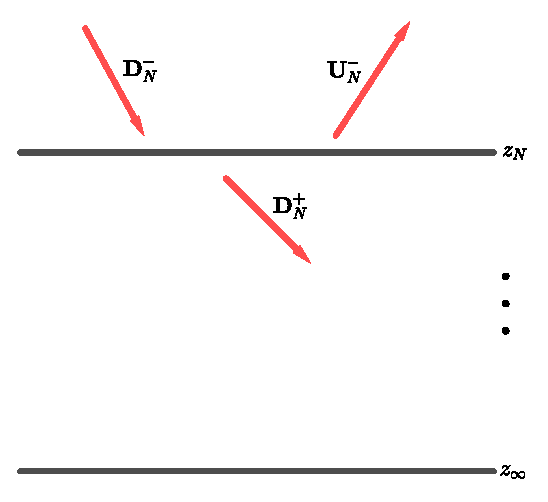
\includegraphics[scale=1]{ondas_em_zn}
\caption{\textit{Ondas ascendentes e descendentes na \'ultima interface. Observe que n\~ao h\'a ondas ascendentes depois da \'ultima camada}.}
\label{fig.ondas_em_zn}
\end{figure}

Substituindo a equa\c{c}\~ao \ref{eq.inversa_matriz_salto} na equa\c{c}\~ao anterior, temos
\begin{align*}
\begin{pmatrix}
\mathbf{U}_N^-\\
\mathbf{D}_N^-
\end{pmatrix}
&=
\begin{pmatrix}
J_{A,N}^\top&-J_{B,N}^\top\\
-J_{B,N}^\top&J_{A,N}^\top
\end{pmatrix}
\,
\begin{pmatrix}
0\\
\mathbf{D}_N^+
\end{pmatrix}\\\\
&=
\begin{pmatrix}
-J_{B,N}^\top \mathbf{D}_N^+\\
 J_{A,N}^\top \mathbf{D}_N^+
\end{pmatrix},
\end{align*}
ou seja,
\begin{align*}
\mathbf{U}_N^-&=-J_{B,N}^\top J_{A,N}^{-\top}\mathbf{D}_N^-\\
\mathbf{D}_N^+&=J_{A,N}^{-\top}\mathbf{D}_N^-.
\end{align*}
Assim, vemos que para computar uma onda refletida, ou seja, uma onda ascendente a partir de uma interface entre camadas, usamos uma \textit{matriz de reflex\~ao} que fica definida como
\begin{equation}\label{eq.reflexao_N}
\Gamma_N=-J_{B,N}^\top J_{A,N}^{-\top}.
\end{equation} 
Analogamente, vemos que para computar uma onda transmitida, ou seja, uma onda descendente a partir de uma interface entre camadas, usamos uma \textit{matriz de transmiss\~ao} que fica definida como
\begin{equation}\label{eq.transmissao_N}
T_N=J_{A,N}^{-\top}.
\end{equation} 

\subsubsection{Reflex\~ao e Transmiss\~ao numa Interface Qualquer}
Definimos a espessura de uma camada, a partir da interface superior, como
\begin{equation}
\Delta\,z_m=z_{m+1}-z_m,\qquad m=1,2,...,N-1,
\end{equation}
e temos que uma onda se propagando da interface na profundidade $z_m$ at\'e a interface em $z_{m+1}$ percorre uma profundidade total $\Delta\,z_m$. O valor dessa onda no fim da trajet\'oria, quando $z=z_{m+1}$, \'e aproximadamente igual a $\mathbf{\Psi}^-_{m+1}$, conforme a figura \ref{fig.N_interfaces}. Assim, usando a solu\c{c}\~ao \ref{eq.solucao_psi} podemos escrever
\begin{equation}\label{eq.solucao_delta_zm}
\mathbf{\Psi}^-_{m+1}=e^{-i\,\omega\tilde{\Lambda}_m\Delta\,z_m}\mathbf{\Psi}^+_m.
\end{equation}

\begin{figure}
\centering
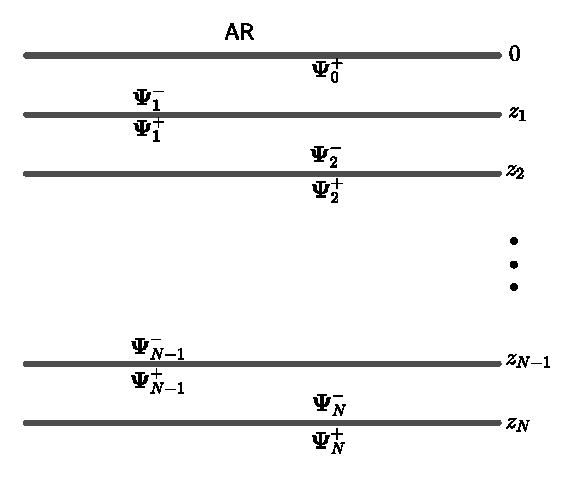
\includegraphics[scale=1]{n_interfaces}
\caption{\textit{Visualiza\c{c}\~ao de $N$ interfaces em subsuperf\'icie e a nota\c{c}\~ao das ondas nas proximadades de cada interface.}}
\label{fig.N_interfaces}
\end{figure}

Sabendo que essa onda se propagando na camada abaixo da interface em $z_m$ veio da camada anterior, podemos usar a matriz de salto na equa\c{c}\~ao \ref{eq.psi_matriz_salto} e escrever
\begin{align}\label{eq.salto_m}
\mathbf{\Psi}^+_{m}&=J_m\,\mathbf{\Psi}^-_m.
\end{align}
Substituindo a equa\c{c}\~ao \ref{eq.salto_m} na equa\c{c}\~ao \ref{eq.solucao_delta_zm}, temos
\begin{align}\label{eq.psi_m-}\nonumber
\mathbf{\Psi}^-_{m+1}&=e^{-i\,\omega\tilde{\Lambda}_m\Delta\,z_m}\mathbf{\Psi}^+_m\\\nonumber
\mathbf{\Psi}^-_{m+1}&=e^{-i\,\omega\tilde{\Lambda}_m\Delta\,z_m}J_m\,\mathbf{\Psi}^-_m\\
\mathbf{\Psi}^-_m&=J^{-1}_me^{i\,\omega\tilde{\Lambda}_m\Delta\,z_m}\mathbf{\Psi}^-_{m+1}
\end{align}
Substituindo a equa\c{c}\~ao \ref{eq.definicao_psi} e a equa\c{c}\~ao \ref{eq.inversa_matriz_salto} na equa\c{c}\~ao \ref{eq.psi_m-}, temos
\begin{align}\label{eq.refle_trans_1}
\mathbf{U}_m^-&=J^\top_{A,m}e^{i\,\omega\Lambda_m\Delta\,z_m}\mathbf{U}^-_{m+1}-J^\top_{B,m}e^{-i\,\omega\Lambda_m\Delta\,z_m}\mathbf{D}^-_{m+1}\\\nonumber\\\label{eq.refle_trans_2}
\mathbf{D}_m^-&=-J^\top_{B,m}e^{i\,\omega\Lambda_m\Delta\,z_m}\mathbf{U}^-_{m+1}+J^\top_{A,m}e^{-i\,\omega\Lambda_m\Delta\,z_m}\mathbf{D}^-_{m+1}.
\end{align}
Assim como definimos matriz de reflex\~ao para a \'ultima interface em $z_N$, podemos definir a matriz de reflex\~ao para uma interface qualquer, ou seja,
\begin{equation}\label{eq.reflexao_m+1}
\mathbf{U}^-_{m+1}=\Gamma_{m+1}\mathbf{D}^-_{m+1}.
\end{equation}
Substituindo a equa\c{c}\~ao \ref{eq.reflexao_m+1} na equa\c{c}\~ao \ref{eq.refle_trans_1} e na equa\c{c}\~ao \ref{eq.refle_trans_2}, temos
\begin{align}\label{eq.refle_trans_3}
\mathbf{U}_m^-&=(J^\top_{A,m}e^{i\,\omega\Lambda_m\Delta\,z_m}\Gamma_{m+1}-J^\top_{B,m}e^{-i\,\omega\Lambda_m\Delta\,z_m})\mathbf{D}^-_{m+1}\\\nonumber\\\label{eq.refle_trans_4}
\mathbf{D}_m^-&=(-J^\top_{B,m}e^{i\,\omega\Lambda_m\Delta\,z_m}\Gamma_{m+1}+J^\top_{A,m}e^{-i\,\omega\Lambda_m\Delta\,z_m})\mathbf{D}^-_{m+1}\,.
\end{align}
Substituindo a equa\c{c}\~ao \ref{eq.refle_trans_4} na equa\c{c}\~ao \ref{eq.refle_trans_3}, temos
\begin{align*}
\mathbf{U}_m^-&=(J^\top_{A,m}e^{i\,\omega\Lambda_m\Delta\,z_m}\Gamma_{m+1}-J^\top_{B,m}e^{-i\,\omega\Lambda_m\Delta\,z_m})\\
&\,\,\cdot\,\,(-J^\top_{B,m}e^{i\,\omega\Lambda_m\Delta\,z_m}\Gamma_{m+1}+J^\top_{A,m}e^{-i\,\omega\Lambda_m\Delta\,z_m})^{-1}\mathbf{D}_m^-\,,
\end{align*}
de onde podemos concluir que a matriz de reflex\~ao em uma interface em $z_m$ qualquer \'e dada por
\begin{align*}
\Gamma_{m}&=(J^\top_{A,m}e^{i\,\omega\Lambda_m\Delta\,z_m}\Gamma_{m+1}-J^\top_{B,m}e^{-i\,\omega\Lambda_m\Delta\,z_m})\\
&\,\,\cdot\,\,(-J^\top_{B,m}e^{i\,\omega\Lambda_m\Delta\,z_m}\Gamma_{m+1}+J^\top_{A,m}e^{-i\,\omega\Lambda_m\Delta\,z_m})^{-1},
\end{align*}
ou
\begin{align}\nonumber
\Gamma_{m}&=(J^\top_{A,m}e^{i\,\omega\Lambda_m\Delta\,z_m}\Gamma_{m+1}e^{i\,\omega\Lambda_m\Delta\,z_m}-J^\top_{B,m})\\\label{eq.matriz_reflexao_m}
&\,\,\cdot\,\,(-J^\top_{B,m}e^{i\,\omega\Lambda_m\Delta\,z_m}\Gamma_{m+1}e^{i\,\omega\Lambda_m\Delta\,z_m}+J^\top_{A,m})^{-1}.
\end{align}
Quando uma onda atinge uma interface, al\'em da possibilidade de reflex\~ao h\'a tamb\'em a possibilidade de trasmiss\~ao da onda para a camada inferior. De maneira an\'aloga ao desenvolvido para reflex\~ao de ondas, podemos deduzir a matriz para a transmiss\~ao de ondas em uma interface qualquer, que \'e dada por
\begin{equation}\label{eq.matriz_transmissao_m}
T_m=T_{m+1}e^{i\,\omega\,\Lambda\Delta\,z_m}(-J^\top_{B,m}e^{i\,\omega\Lambda_m\Delta\,z_m}\Gamma_{m+1}e^{i\,\omega\Lambda_m\Delta\,z_m}+J^\top_{A,m})^{-1}.
\end{equation}
A validade das equa\c{c}\~oes \ref{eq.matriz_reflexao_m} e \ref{eq.matriz_transmissao_m} para qualquer interface pode ser demonstrada por indu\c{c}\~ao sobre $m$, e todas as matrizes de reflex\~ao e transmiss\~ao podem ser computadas por recurss\~ao partindo das equa\c{c}\~oes \ref{eq.reflexao_N} e \ref{eq.transmissao_N}.

\section{Solu\c{c}\~ao na Presen\c{c}a de Fonte}\label{sec.presenca_fonte}
Em prospec\c{c}\~ao de petr\'oleo s\~ao utilizadas alguns tipos de fontes de ondas, atrav\'es das quais se faz um mapeamento das caracter\'isticas das camadas de subsuperf\'icie. Segundo \cite{dobrin_88}, esses tipos de fontes podem ser uma queda de peso, um caminh\~ao \textit{vibroseis}, explosivos e canh\~ao de ar, esta \'ultima fonte utilizada em prospec\c{c}\~ao mar\'itima. Sendo assim, vamos desenvolver uma solu\c{c}\~ao para o nosso problema considerando agora a presen\c{c}a de uma fonte.

Considere ainda a equa\c{c}\~ao \ref{eq.matricial} com o sobrescrito $m$ omitido. Uma fonte $\mathbf{S}$ localizada numa profundidade $z_s$ pode ser representada na forma
\begin{equation}\label{eq.fonte_geral}
\mathbf{S}=\mathbf{S}_0\delta(z-z_s)+\mathbf{S}_1\delta^\prime(z-z_s),
\end{equation}
onde $\mathbf{S}_0$ e $\mathbf{S}_1$ n\~ao dependem da profundidade e $\delta$ \'e a fun\c{c}\~ao \textit{Delta de Dirac} conforme a subse\c{c}\~ao \ref{sec.dirac}. Fontes que s\~ao distribu\'idas ao longo da profundidade podem, geralmente, ser sintetizadas por superposi\c{c}\~ao de fontes do tipo $\mathbf{S}_0$ e $\mathbf{S}_1$. 

Uma solu\c{c}\~ao por ser escrita como a combina\c{c}\~ao de uma solu\c{c}\~ao inicial sofrendo a a\c{c}\~ao de alguma fonte, ou seja,
\begin{equation}\label{eq.solucao_inicial_fonte}
\mathbf{\Phi}=\mathbf{\Phi}_0+\mathbf{S}_1\delta(z-z_s).
\end{equation} 
Substituindo a equa\c{c}\~ao \ref{eq.solucao_inicial_fonte} e a equa\c{c}\~ao \ref{eq.fonte_geral} na equa\c{c}\~ao \ref{eq.matricial}, temos
\begin{equation}\label{eq.matricial_fonte}
\frac{d\,\mathbf{\Phi}_0}{d\,z}=-i\,\omega\,M\,\mathbf{\Phi}_0+\left[\mathbf{S}_0-i\,\omega\,M\,\mathbf{S}_1\right]\,\delta(z-z_s),
\end{equation}
e por simplicidade, vamos escrever
\begin{equation}\label{eq.fonte_simplificada}
i\,\omega\,M\,\mathbf{S}_1-\mathbf{S}_0=
\begin{pmatrix}
\mathbf{S}_A\\
\mathbf{S}_B
\end{pmatrix}.
\end{equation}
Considerando a exist\^encia de uma interface imagin\'aria na profundidade $z_s$ da fonte, podemos determinar as condi\c{c}\~oes de salto no local da fonte da mesma forma que estudamos as condi\c{c}\~oes de salto nas interfaces que separam as camadas. Assim, integrando a equa\c{c}\~ao \ref{eq.matricial_fonte} no intervalo que come\c{c}a imediatamente acima da interface imagin\'aria da fonte $z_s^-$, e termina imediatamente abaixo da interface imagin\'aria da fonte em $z_s^+$, e substituindo a equa\c{c}\~ao \ref{eq.fonte_simplificada}, temos como solu\c{c}\~ao
\begin{equation*}
\mathbf{\Phi}_0(z_s^-)=\mathbf{\Phi}_0(z_s^+)+
\begin{pmatrix}
\mathbf{S}_A\\
\mathbf{S}_B
\end{pmatrix}.
\end{equation*}
Substituindo a equa\c{c}\~ao \ref{eq.solucao_inicial_fonte} e considerando as caracter\'isticas da fun\c{c}\~ao Delta de Dirac, temos a seguinte condi\c{c}\~ao de salto na profundidade da fonte
\begin{equation}\label{eq.salto_zs}
\mathbf{\Phi}(z_s^-)=\mathbf{\Phi}(z_s^+)+
\begin{pmatrix}
\mathbf{S}_A\\
\mathbf{S}_B
\end{pmatrix}.
\end{equation}

Vamos agora inserir uma interface imagin\'aria imediatamente abaixo da fonte, em $z=z_s^+$ e utilizar os m\'etodos do cap\'itulo \ref{sec.ausencia_fonte} para computar a matriz de reflex\~ao $\Gamma_s\equiv\Gamma(z_s^+)$ a partir do topo desta camada. J\'a que a interface em $z_s^+$ \'e fict\'icia, as propriedades do meio s\~ao iguais acima e abaixo dessa interface, assim temos que $L_2^+=L_2^-$ e $L_1^+=L_1^-$. Substituindo essas identidades nas equa\c{c}\~oes \ref{eq.j_a} e \ref{eq.j_b}, temos
\begin{align}\label{eq.j_a_ficticia}
J_A&=\frac{1}{2}\left[(L_2)^\top L_1+(L_1)^\top L_2\right]\\\label{eq.j_b_ficticia}
J_B&=\frac{1}{2}\left[(L_2)^\top L_1-(L_1)^\top L_2\right].
\end{align}
Substituindo as equa\c{c}\~oes \ref{eq.l1l2} e \ref{eq.l2l1} nas equa\c{c}\~oes \ref{eq.j_a_ficticia} e \ref{eq.j_b_ficticia}, obtemos que
\begin{align*}
J_A&=I\\
J_B&=0.
\end{align*}
Desta forma, a onda ascendente $\mathbf{U}(z_s^+)$ e a onda descendente $\mathbf{D}(z_s^+)$ a partir da interface em $z_s^+$ podem ser introduzidas na equa\c{c}\~ao \ref{eq.definicao_psi} para obtermos
\begin{equation*}
\mathbf{\Psi}(z_s^+)=
\begin{pmatrix}
\mathbf{U}(z_s^+)\\
\mathbf{D}(z_s^+)
\end{pmatrix}.
\end{equation*}
Substituindo a equa\c{c}\~ao \ref{eq.reflexao_m+1} na equa\c{c}\~ao acima, temos
\begin{equation}\label{eq.Psi_descendente}
\mathbf{\Psi}(z_s^+)=
\begin{pmatrix}
\Gamma_s\mathbf{D}(z_s^+)\\
\mathbf{D}(z_s^+)
\end{pmatrix},
\end{equation}
pois as ondas est\~ao numa mesma camada e da\'i usamos que
\begin{align*}
\mathbf{U}^-(z_s^+)&=\mathbf{U}(z_s^+)\\
\mathbf{D}^-(z_s^+)&=\mathbf{D}(z_s^+).
\end{align*}
Multiplicando a equa\c{c}\~ao \ref{eq.salto_zs} por $L^{-1}$ e substituindo a equa\c{c}\~ao \ref{eq.Phi}, obtemos
\begin{equation}\label{eq.Psi_salto_zs}
\mathbf{\Psi}(z_s^-)=\mathbf{\Psi}(z_s^+)+L^{-1}
\begin{pmatrix}
\mathbf{S}_A\\
\mathbf{S}_B
\end{pmatrix}.
\end{equation}
Substituindo a express\~ao para $L^{-1}$ dada pela equacao \ref{eq.L^-1}, juntamente com a equa\c{c}\~ao \ref{eq.Psi_descendente} na equa\c{c}\~ao \ref{eq.Psi_salto_zs}, temos
\begin{equation}\label{eq.solucao_phi_zs-}
\mathbf{\Psi}(z_s^-)=
\begin{pmatrix}
\Gamma_s\mathbf{D}(z_s^+)\\
\mathbf{D}(z_s^+)
\end{pmatrix}
+
\frac{1}{\sqrt{2}}\,
\begin{pmatrix}
L_2^\top\mathbf{S}_A+L_1^\top\mathbf{S}_B\\
L_2^\top\mathbf{S}_A-L_1^\top\mathbf{S}_B
\end{pmatrix}.
\end{equation}
Admitindo que a fonte esteja no interior da primeira camada, ou seja, $0<z_s<z_1$, a solu\c{c}\~ao dada pela equa\c{c}\~ao \ref{eq.solucao_phi_zs-} \'e propagada para cima a partir de $z_s^-$ usando a equa\c{c}\~ao \ref{eq.solucao_psi}, e o salto atrav\'es das interfaces entre camadas \'e dado pela equa\c{c}\~ao \ref{eq.psi_matriz_salto} at\'e que a onda atinja a interface terra/ar em $z=0^+$. Assim,
\begin{equation*}
\mathbf{\Psi}(0^+)=e^{-i\,\omega\,\tilde{\mathbf{\Lambda}}\,(0^+-z_s^-)}\,\mathbf{\Psi}(z_s^-),
\end{equation*}
e podemos usar as $n$ condi\c{c}\~oes de fronteira em $z=0$ para determinarmos as $n$ inc\'ognitas de $\mathbf{D}_s$. Os demais termos da solu\c{c}\~ao s\~ao conhecidos. A diferen\c{c}a $z_s^--0^+$ corresponde \`a profundidade da fonte, assim a solu\c{c}\~ao anterior pode ser reescrita como
\begin{align*}
\mathbf{\Psi}(0^+)&=e^{-i\,\omega\,\tilde{\mathbf{\Lambda}}\,(-z_s)}\,\mathbf{\Psi}(z_s^-)\\\\
\mathbf{\Psi}(0^+)&=
\begin{pmatrix}
e^{i\,\omega\,\mathbf{\Lambda}\,z_s}&\mathbf{0}\\
\mathbf{0}&e^{-i\,\omega\,\mathbf{\Lambda}\,z_s}
\end{pmatrix}
\mathbf{\Psi}(z_s^-).
\end{align*}
Substituindo a equa\c{c}\~ao \ref{eq.solucao_phi_zs-} na equa\c{c}\~ao acima, temos
\begin{equation}\label{eq.Psi_zero+}
\mathbf{\Psi}(0^+)=
\begin{pmatrix}
e^{i\,\omega\,\mathbf{\Lambda}\,z_s}\,\Gamma_s\mathbf{D}(z_s^+)\\
e^{-i\,\omega\,\mathbf{\Lambda}\,z_s}\,\mathbf{D}(z_s^+)
\end{pmatrix}
+
\frac{1}{\sqrt{2}}\,
\begin{pmatrix}
e^{i\,\omega\,\mathbf{\Lambda}\,z_s}\,(L_2^\top\mathbf{S}_A+L_1^\top\mathbf{S}_B)\\
e^{-i\,\omega\,\mathbf{\Lambda}\,z_s}\,(L_2^\top\mathbf{S}_A-L_1^\top\mathbf{S}_B)
\end{pmatrix},
\end{equation}
e teremos os valores de cada campo quando as ondas retornarem \`a superf\'icie.


%\chapter{Solu\c{c}\~ao das Equa\c{c}\~oes \ref{eq.matricial_1}-\ref{eq.matricial_2} na Aus\^encia de Fonte}

Vamos determinar inicialmente a solu\c{c}\~ao das equa\c{c}\~oes \ref{eq.matricial_1}-\ref{eq.matricial_2} considerando o meio homog\^eneo e livre de fonte. Assim, temos que $\mathbf{S}^{(m)}=0$ para $m=1,2,3,4\,$ e a matriz $\mathbf{M}^{(m)}$ \'e constante onde as submatrizes na diagonal principal s\~ao nulas e as submatrizes na diagonal secund\'aria s\~ao sim\'etricas. 

\section{Ondas Ascendentes e Ondas Descendentes}

Vamos redefinir o vetor de ondas como
\begin{equation}\label{eq.Phi}
\mathbf{\Phi}=L\,\mathbf{\Psi}.
\end{equation}
Substituindo a equa\c{c}\~ao \ref{eq.Phi} na equa\c{c}\~ao \ref{eq.matricial}, temos
\begin{equation}\label{eq.matricial_sem_fonte}
\frac{\partial\,\mathbf{\Psi}}{\partial\,z} =-\,i\,\omega\,L^{-1}M\,L\,\mathbf{\Psi},
\end{equation}
onde o sobrescrito $m$ est\'a sendo omitido por quest\~ao de simplicidade.
De acordo com a subse\c{c}\~ao \ref{sec.diagonalizacao_ursin}, temos que as matrizes $M$ e $\tilde{\Lambda}$ s\~ao semelhantes, assim
\begin{equation*}
\tilde{\Lambda}=L^{-1}M\,L.
\end{equation*}
Substituindo $\tilde{\Lambda}$ na equa\c{c}\~ao \ref{eq.matricial_sem_fonte}, temos
\begin{equation}\label{eq.matricial_sem_fonte_2}
\frac{\partial\,\mathbf{\Psi}}{\partial\,z} =-\,i\,\omega\,\tilde{\Lambda}\,\mathbf{\Psi}.
\end{equation}
Ainda de acordo com a subse\c{c}\~ao \ref{sec.diagonalizacao_ursin}, podemos escrever
\begin{equation}
\tilde{\Lambda}=
\begin{pmatrix}
\Lambda&0\\
0&-\Lambda
\end{pmatrix},
\end{equation}
onde $\Lambda$ \'e uma submatriz diagonal contendo os autovalores $q_i$.
Definindo
\begin{equation}
\mathbf{\Psi}=
\begin{pmatrix}
\mathbf{U}\\
\mathbf{D}
\end{pmatrix}
\end{equation}
e usando o fato de que $\tilde{\Lambda}$ \'e uma matriz diagonal, podemos resolver a equa\c{c}\~ao diferencial \ref{eq.matricial_sem_fonte_2} e expressar a solu\c{c}\~ao na forma
\begin{align*}
\Psi(z)&=e^{-i\,\omega\,\tilde{\Lambda}(z-z_0)}\Psi(z_0)\\
&=\begin{pmatrix}
e^{-i\,\omega\,\Lambda(z-z_0)}\,\mathbf{U}(z_0)\\
e^{i\,\omega\,\Lambda(z-z_0)}\,\,\,\mathbf{D}(z_0)
\end{pmatrix}.
\end{align*}
Desta maneira, $\mathbf{U}$ representa ondas ascendentes e $\mathbf{D}$ representa ondas descendentes, $z_0$ \'e um ponto fixo na mesma regi\~ao livre de fonte de $z$ e $e^{\pm i\,\omega\,\Lambda(z-z_0)}$ \'e uma matriz diagonal onde o $i$-ésimo elemento da diagonal principal \'e dado por $e^{\pm i\,\omega\,q_i(z-z_0)}$. 

\section{Matriz de Salto para Camadas Estratificadas}

A profundidade onde encontra-se uma interface entre duas camadas estratificadas ser\'a denotada por $\overline{z}$, onde as quantidades avaliadas exatamente abaixo da interface ser\'a denotada por $\overline{z}^+$ e as quantidades avaliadas exatamente acima da interface ser\'a denotada por $\overline{z}^-$.mesclado
%\input{solucao_presenca_fonte}mesclado
\chapter{Sistema de EDO's do Efeito Magneto-El\'astico}\label{sec.trans_edp_2_edo}
Neste cap\'itulo vamos aplicar algumas t\'ecnicas como rota\c{c}\~ao do sistema de coordenadas e Transformadas Laterais de Fourier em EDP's da magneto-elasticidade para que as mesmas possam ser escritas como um sistema de EDO's.

\section{Transformando EDP's em EDO's}

Segundo \cite{eringen_1963}, o acoplamento entre ondas eletromagn\'eticas e el\'asticas se propagando no subsolo caracteriza o efeito magneto-el\'astico, e esse acoplamento pode ser modelado matematicamente atrav\'es de um sistema de equa\c{c}\~oes diferencias parciais. Conforme \cite{pinho_2018}, podemos aplicar uma s\'erie de hip\'oteses oriundas das caracter\'isticas f\'isicas do efeito magneto-el\'astico, as quais visam simplificar e linearizar essas EDP's de forma que as mesmas possam receber um tratamento matem\'atico anal\'itico adequado, para em seguida se obter numericamente os valores dos campos eletromagn\'eticos e el\'asticos envolvidos no sistema. 
\begin{align}\label{eq.mag_ela_1}
\nabla\times\mathbf{{E}}&=i\,\omega\,\mu_0\mathbf{{H}}\\\nonumber\\\label{eq.mag_ela_2}
\nabla\times\mathbf{{H}}&=(\sigma-i\,\epsilon\,\omega)\,\mathbf{{E}}+\mathbf{{v}}\times\sigma\mu_0\mathbf{H}^0+\mathbf{j}\\\nonumber\\\label{eq.mag_ela_3}
-i\,\omega\rho\,\mathbf{{v}}&=\nabla\cdot{\tau} + \mathbf{{F}}\\\nonumber\\\label{eq.mag_ela_4}
{\tau}&=\lambda\,\nabla\cdot\mathbf{{u}}\cdot\,I + G\,(\nabla\,\mathbf{{u}}+\nabla\mathbf{{u}}^\top)\\\nonumber\\\label{eq.mag_ela_5}
\nabla\cdot\mathbf{{H}}&=0.
\end{align}
Estas equa\c{c}\~oes est\~ao no dom\'inio da frequ\^encia $\omega$, a depend\^encia do tempo \'e dada por $e^{-i\,\omega\,t}$ e 
\begin{itemize}
\item $\mathbf{{E}}$ \'e o campo el\'etrico,
\item $\mathbf{{B}}$ \'e o campo magn\'etico,
\item $\mathbf{{D}}$ \'e o campo de densidade de fluxo el\'etrico,
\item $\mathbf{{H}}$ \'e o campo magn\'etico auxiliar,
\item $\tau$ \'e o tensor de tens\~oes,
\item $\mathbf{{u}}$ \'e o deslocamento do meio,
\item $\mathbf{{v}}$ \'e a velocidade de deslocamento do meio,
\item $\mathbf{{F}}$ \'e uma for\c{c}a aplicada ao meio,
\item $\mathbf{H}^0$ \'e campo geomagn\'etico,
\item $i$ \'e um n\'umero complexo,
\item $\omega$ \'e a frequ\^encia temporal,
\item $\mu_0$ \'e a permeabilidade magn\'etica no v\'acuo,
\item $\sigma$ \'e a condutividade do meio,
\item $\epsilon$ \'e a permissividade el\'etrica do meio,
\item $\rho$ \'e a densidade do meio,
\item $\lambda$ e $G$ s\~ao par\^ametros de Lam\`e.
\end{itemize}
Vamos definir $\overline{\sigma}=(\sigma-i\,\epsilon\,\omega)$. No subsolo, por conta do regime quasi-estacion\'ario, $(\sigma>>\epsilon\,\omega)$  e  temos $\overline{\sigma}=\sigma$. No ar, a condutividade \'e zero e a permeabilidade el\'etrica \'e pr\'oxima a do v\'acuo $\epsilon_0$, assim temos $\overline{\sigma}=-i\,\epsilon_0\omega$.

No formato matricial, a equa\c{c}\~ao \ref{eq.mag_ela_1} pode ser escrita como
\begin{equation*}
\begin{pmatrix}
\frac{\partial\,E_3}{\partial\,y}-\frac{\partial\,E_2}{\partial\,z}\\
\frac{\partial\,E_1}{\partial\,z}-\frac{\partial\,E_3}{\partial\,x}\\
\frac{\partial\,E_2}{\partial\,x}-\frac{\partial\,E_1}{\partial\,y}
\end{pmatrix}
=
i\,\omega\,\mu_0\,
\begin{pmatrix}
H_1\\
H_2\\
H_3
\end{pmatrix}.
\end{equation*}
Aplicando as transformadas laterais de Fourier, dada em \ref{eq.trans_fourier_1}, temos
\begin{empheq}[left=\empheqlbrace]{align*}
i\,k_y\widehat{E}_3-\frac{\partial\,\widehat{E}_2}{\partial\,z}&=i\,\omega\,\mu_0\widehat{H}_1\\
\frac{\partial\,\widehat{E}_1}{\partial\,z}-i\,k_x\widehat{E}_3&=i\,\omega\,\mu_0\widehat{H}_2\\
i\,k_x\widehat{E}_2-i\,k_y\widehat{E}_1&=i\,\omega\,\mu_0\widehat{H}_3.
\end{empheq} 
Rotacionando o sistema de forma que a primeira coordenada esteja orientada no sentido do vetor de onda horizontal, usando o operador dado pela equa\c{c}\~ao \ref{eq.operador_rotacao}, e fazendo as simplifica\c{c}\~oes, temos
\begin{empheq}[left=\empheqlbrace]{align*}
-\frac{\partial\,\tilde{E}_2}{\partial\,z}&=i\,\omega\,\mu_0\tilde{H}_1\\
\frac{\partial\,\tilde{E}_1}{\partial\,z}&=i\,\omega\,\mu_0\tilde{H}_2+i\,k\tilde{E}_3\\
i\,\tilde{E}_2&=\frac{i\,\omega\,\mu_0}{k}\tilde{H}_3.
\end{empheq}

Observando que $\mathbf{v}=-i\,\omega\mathbf{u}$ depois de aplicada a transformada de Fourier no tempo, a equa\c{c}\~ao \ref{eq.mag_ela_2} pode ser escrita como
\begin{equation*}
\begin{pmatrix}
\frac{\partial\,H_3}{\partial\,y}-\frac{\partial\,H_2}{\partial\,z}\\
\frac{\partial\,H_1}{\partial\,z}-\frac{\partial\,H_3}{\partial\,x}\\
\frac{\partial\,H_2}{\partial\,x}-\frac{\partial\,H_1}{\partial\,y}
\end{pmatrix}
=
(\sigma-i\,\epsilon\,\omega)\,
\begin{pmatrix}
E_1\\
E_2\\
E_3
\end{pmatrix}
-i\,\omega\,\sigma\,\mu_0
\begin{pmatrix}
u_2H_3^0-u_3H_2^0\\
u_3H_1^0-u_1H_3^0\\
u_1H_2^0-u_2H_1^0
\end{pmatrix}
+
\begin{pmatrix}
j_1\\
j_2\\
j_3
\end{pmatrix}.
\end{equation*}
Aplicando as transformadas laterais de Fourier conforme a equa\c{c}\~ao \ref{eq.trans_fourier_1}, temos
\begin{empheq}[left=\empheqlbrace]{align*}
i\,k_y\widehat{H}_3-\frac{\partial\,\widehat{H}_2}{\partial\,z}&=(\sigma-i\,\epsilon\,\omega)\,\widehat{E}_1-i\,\omega\,\sigma\,\mu_0(u_2H_3^0-u_3H_2^0)+\widehat{j}_1\\
\frac{\partial\,\widehat{H}_1}{\partial\,z}-i\,k_x\widehat{H}_3&=(\sigma-i\,\epsilon\,\omega)\,\widehat{E}_2-i\,\omega\,\sigma\,\mu_0(u_3H_1^0-u_1H_3)+\widehat{j}_2\\
i\,k_x\widehat{H}_2-i\,k_y\widehat{H}_1&=(\sigma-i\,\epsilon\,\omega)\,\widehat{E}_3-i\,\omega\,\sigma\,\mu_0(u_1H_2^0-u_2H_1^0)+\widehat{j}_3.
\end{empheq}
Rotacionando o sistema usando o operador dado pela equa\c{c}\~ao \ref{eq.operador_rotacao}, e fazendo as simplifica\c{c}\~oes, temos
\begin{empheq}[left=\empheqlbrace]{align*}
-\frac{\partial\,\tilde{H}_2}{\partial\,z}&=(\sigma-i\,\epsilon\,\omega)\,\tilde{E}_1-i\,\omega\,\sigma\,\mu_0\,\tilde{H}_3^0\tilde{u}_2+i\,\omega\,\sigma\,\mu_0\,\tilde{H}_2^0\tilde{u}_3+\tilde{j}_1\\
\frac{\partial\,\tilde{H}_1}{\partial\,z}&=(\sigma-i\,\epsilon\,\omega)\,\tilde{E}_2+i\,k\,\tilde{H}_3-i\,\omega\,\sigma\,\mu_0\,\tilde{H}_1^0\tilde{u}_3+i\,\omega\,\sigma\,\mu_0\,\tilde{H}_3^0\tilde{u}_1+\tilde{j}_2\\
i\,k\,\tilde{H}_2&=(\sigma-i\,\epsilon\,\omega)\tilde{E}_3-i\,\omega\,\sigma\,\mu_0\,(\tilde{H}_2^0\tilde{u}_1-\tilde{H}_1^0\tilde{u}_2)+\tilde{j}_3.
\end{empheq}

A equa\c{c}\~ao \ref{eq.mag_ela_3} pode ser reescrita como

\begin{empheq}[left=\empheqlbrace]{align*}
-\omega^2\rho\,u_1&=\frac{\partial \tau_{11}}{\partial\,x}+\frac{\partial \tau_{12}}{\partial\,y}+\frac{\partial \tau_{13}}{\partial\,z}+F_1\\
-\omega^2\rho\,u_2&=\frac{\partial \tau_{21}}{\partial\,x}+\frac{\partial \tau_{22}}{\partial\,y}+\frac{\partial \tau_{23}}{\partial\,z}+F_2\\
-\omega^2\rho\,u_3&=\frac{\partial \tau_{31}}{\partial\,x}+\frac{\partial \tau_{32}}{\partial\,y}+\frac{\partial \tau_{33}}{\partial\,z}+F_3
\end{empheq}
Aplicando as transformadas laterais de Fourier, temos
\begin{empheq}[left=\empheqlbrace]{align*}
-\omega^2\rho\,\widehat{u}_1&=i\,k_x\widehat{\tau}_{11}+i\,k_y\widehat{\tau}_{12}+\frac{\partial\widehat{\tau}_{13}}{\partial\,z}+\widehat{F}_1\\
-\omega^2\rho\,\widehat{u}_2&=i\,k_x\widehat{\tau}_{21}+i\,k_y\widehat{\tau}_{22}+\frac{\partial\widehat{\tau}_{23}}{\partial\,z}+\widehat{F}_2\\
-\omega^2\rho\,\widehat{u}_3&=i\,k_x\widehat{\tau}_{31}+i\,k_y\widehat{\tau}_{32}+\frac{\partial\widehat{\tau}_{33}}{\partial\,z}+\widehat{F}_3.
\end{empheq}
Aplicando a rota\c{c}\~ao e simplificando as equa\c{c}\~oes, temos
\begin{empheq}[left=\empheqlbrace]{align*}
-\omega^2\rho\,\tilde{u}_1&=i\,k\tilde{\tau}_{11}+\frac{\partial\tilde{\tau}_{13}}{\partial\,z}+\tilde{F}_1\\
-\omega^2\rho\,\tilde{u}_2&=i\,k\tilde{\tau}_{12}+\frac{\partial\tilde{\tau}_{23}}{\partial\,z}+\tilde{F}_2\\
-\omega^2\rho\,\tilde{u}_3&=i\,k\tilde{\tau}_{13}+\frac{\partial\tilde{\tau}_{33}}{\partial\,z}+\tilde{F}_3.
\end{empheq}

A equa\c{c}\~ao \ref{eq.mag_ela_4} pode ser reescrita como
\begin{equation*}
\begin{pmatrix}
\tau_{11}&\tau_{12}&\tau_{13}\\
\tau_{21}&\tau_{22}&\tau_{23}\\
\tau_{31}&\tau_{32}&\tau_{33}
\end{pmatrix}
=
\lambda\,\left(\frac{\partial\,u_1}{\partial\,x}+\frac{\partial\,u_2}{\partial\,y}+\frac{\partial\,u_3}{\partial\,z}\right)\,I+G\,
\begin{pmatrix}
2\,\frac{\partial\,u_1}{\partial\,x}&\frac{\partial\,u_1}{\partial\,y}+\frac{\partial\,u_2}{\partial\,x}&\frac{\partial\,u_1}{\partial\,z}+\frac{\partial\,u_3}{\partial\,x}\\
\frac{\partial\,u_2}{\partial\,x}+\frac{\partial\,u_1}{\partial\,y}&2\,\frac{\partial\,u_2}{\partial\,y}&\frac{\partial\,u_2}{\partial\,z}+\frac{\partial\,u_3}{\partial\,y}\\
\frac{\partial\,u_3}{\partial\,x}+\frac{\partial\,u_1}{\partial\,z}&\frac{\partial\,u_3}{\partial\,y}+\frac{\partial\,u_2}{\partial\,z}&2\,\frac{\partial\,u_3}{\partial\,z}
\end{pmatrix},
\end{equation*}
onde $I$ \'e uma matriz identidade.
Dada a simetria do tensor $\tau_{ij}$ temos seis equa\c{c}\~oes
\begin{empheq}[left=\empheqlbrace]{align*}
\tau_{11}&=\lambda\,\left(\frac{\partial\,u_1}{\partial\,x}+\frac{\partial\,u_2}{\partial\,y}+\frac{\partial\,u_3}{\partial\,z}\right)+2\,G\,\frac{\partial\,u_1}{\partial\,x}\\
\tau_{12}&=G\,\left(\frac{\partial\,u_1}{\partial\,y}+\frac{\partial\,u_2}{\partial\,x}\right)\\
\tau_{13}&=G\,\left(\frac{\partial\,u_1}{\partial\,z}+\frac{\partial\,u_3}{\partial\,x}\right)\\
\tau_{22}&=\lambda\,\left(\frac{\partial\,u_1}{\partial\,x}+\frac{\partial\,u_2}{\partial\,y}+\frac{\partial\,u_3}{\partial\,z}\right)+2\,G\,\frac{\partial\,u_2}{\partial\,y}\\
\tau_{23}&=G\,\left(\frac{\partial\,u_2}{\partial\,z}+\frac{\partial\,u_3}{\partial\,y}\right)\\
\tau_{33}&=\lambda\,\left(\frac{\partial\,u_1}{\partial\,x}+\frac{\partial\,u_2}{\partial\,y}+\frac{\partial\,u_3}{\partial\,z}\right)+2\,G\,\frac{\partial\,u_3}{\partial\,z}.
\end{empheq}
Aplicando as transformadas laterais de Fourier no sistema acima, temos
\begin{empheq}[left=\empheqlbrace]{align*}
\widehat{\tau}_{11}&=\lambda\,\left(-i\,k_x\widehat{u}_1-i\,k_y\widehat{u}_2+\frac{\partial\,\widehat{u}_3}{\partial\,z}\right)-2\,i\,G\,k_x\widehat{u}_1\\
\widehat{\tau}_{12}&=G\,\left(-i\,k_y\widehat{u}_1-i\,k_x\widehat{u}_2\right)\\
\widehat{\tau}_{13}&=G\,\left(\frac{\partial\,\widehat{u}_1}{\partial\,z}-i\,k_x\widehat{u}_3\right)\\
\widehat{\tau}_{22}&=\lambda\,\left(-i\,k_x\widehat{u}_1-i\,k_y\widehat{u}_2+\frac{\partial\,\widehat{u}_3}{\partial\,z}\right)-2\,i\,G\,k_y\widehat{u}_2\\
\widehat{\tau}_{23}&=G\,\left(\frac{\partial\,\widehat{u}_2}{\partial\,z}-i\,k_y\widehat{u}_3\right)\\
\widehat{\tau}_{33}&=\lambda\,\left(-i\,k_x\widehat{u}_1-i\,k_y\widehat{u}_2+\frac{\partial\,\widehat{u}_3}{\partial\,z}\right)+2\,G\,\frac{\partial\,\widehat{u}_3}{\partial\,z}.
\end{empheq}
E aplicando a rota\c{c}\~ao $\Omega$ na forma dada pela equa\c{c}\~ao \ref{eq.rotacao_tensor}, fazendo as simplifica\c{c}\~oes, finalmente a lei de Hooke se torna
\begin{empheq}[left=\empheqlbrace]{align*}
\tilde{\tau}_{11}&=i\,k(\lambda+2\,G)\,\tilde{u}_1+\lambda\,\frac{\partial\,\tilde{u}_3}{\partial\,z}\\
\tilde{\tau}_{12}&=i\,G\,k\,\tilde{u}_2\\
\tilde{\tau}_{13}&=G\,\frac{\partial\,\tilde{u}_1}{\partial\,z}+i\,G\,k\,\tilde{u}_3\\
\tilde{\tau}_{22}&=\lambda\,\frac{\partial\,\tilde{u}_3}{\partial\,z}+i\,\lambda\,k\,\tilde{u}_1\\
\tilde{\tau}_{23}&=G\,\frac{\partial\,\tilde{u}_2}{\partial\,z}\\
\tilde{\tau}_{33}&=(\lambda+2\,G)\,\frac{\partial\,\tilde{u}_3}{\partial\,z}+i\,\lambda\,k\,\tilde{u}_1.
\end{empheq}
Vimos que as equa\c{c}\~oes \ref{eq.mag_ela_1}, \ref{eq.mag_ela_2}, \ref{eq.mag_ela_3} e \ref{eq.mag_ela_4} escritas no espa\c{c}o horizontal de Fourier e rotacionadas nos fornecem quinze equa\c{c}\~oes. Isolando as vari\'aveis $\tilde{H}_3,\tilde{E}_3,\tilde{\tau}_{11},\tilde{\tau}_{22}$ e $\tilde{\tau}_{12}$, podemos substituir algumas equa\c{c}\~oes em outras e reduzir a quantidade para dez. Fazendo ainda as substitui\c{c}\~oes da vari\'avel $\dot{\tilde{\mathbf{u}}}=-i\,\omega\,\tilde{\mathbf{u}}$, da vagarosidade horizontal conforme a equa\c{c}\~ao \ref{eq.numero_onda_vagarozidade_horizontal} e isolando as derivadas parciais em rela\c{c}\~ao \`a profundidade, temos o seguinte sistema 
\begin{empheq}[left=\empheqlbrace]{align*}
\frac{\partial\,\tilde{E}_1}{\partial\,z}&=\left(i\,\omega\,\mu_0+\frac{i^2\gamma^2\omega^2}{\sigma-i\,\epsilon\,\omega}\right)\,\tilde{H}_2-\frac{i\,\gamma\,\omega\,\sigma\,\mu_0\tilde{H}_2^0}{\sigma-i\,\epsilon\,\omega}\dot{\tilde{u}}_1+\frac{i\,\gamma\,\omega\,\sigma\,\mu_0\tilde{H}_1^0}{\sigma-i\,\epsilon\,\omega}\dot{\tilde{u}}_2+\frac{i\,\gamma\,\omega}{\sigma-i\,\epsilon\,\omega}\,\tilde{j}_3\\\\
\frac{\partial\,\tilde{E}_2}{\partial\,z}&=-i\,\omega\,\mu_0\,\tilde{H}_1\\\\
-\frac{\partial\,\tilde{H}_1}{\partial\,z}&=-\left(\sigma-i\,\epsilon\,\omega+\frac{i^2\gamma^2\omega^2}{i\,\omega\,\mu_0}\right)\,\tilde{E}_2+\sigma\,\mu_0\tilde{H}_3^0\dot{\tilde{u}}_1-\sigma\,\mu_0\tilde{H}_1^0\dot{\tilde{u}}_3-\tilde{j}_2\\\\
\frac{\partial\,\tilde{H}_2}{\partial\,z}&=-\left(\sigma-i\,\epsilon\,\omega\right)\,\tilde{E}_1-\sigma\,\mu_0\tilde{H}_3^0\dot{\tilde{u}}_2+\sigma\,\mu_0\tilde{H}_2^0\dot{\tilde{u}}_3-\tilde{j}_1\\\\
\frac{\partial\,\dot{\tilde{u}}_1}{\partial\,z}&=-i\,\gamma\,\omega\,\dot{\tilde{u}}_3-\frac{i\,\omega}{G}\,\tilde{\tau}_{13}\\\\
\frac{\partial\,\dot{\tilde{u}}_2}{\partial\,z}&=-\frac{i\,\omega}{G}\,\tilde{\tau}_{23}\\\\
\frac{\partial\,\dot{\tilde{u}}_3}{\partial\,z}&=-\frac{i\,\omega}{\lambda+2\,G}\,\tilde{\tau}_{33}-\frac{i\,\omega\,\gamma\,\lambda}{\lambda+2\,G}\,\dot{\tilde{u}}_1\\\\
\frac{\partial\,\tilde{\tau}_{13}}{\partial\,z}&=
\left[\frac{\omega\,\rho}{i}-\frac{i^2\gamma^2\omega}{i}\cdot\frac{\lambda^2-(\lambda+2\,G)^2}{\lambda+2\,G}\right]\,\dot{\tilde{u}}_1-\frac{i\,\omega\,\gamma\,\lambda}{\lambda+2\,G}\,\tilde{\tau}_{33}-\tilde{F}_1\\\\
\frac{\partial\,\tilde{\tau}_{23}}{\partial\,z}&=\left[\frac{\omega\,\rho}{i}+\frac{i^2\gamma^2\omega\,G}{i}\right]\,\dot{\tilde{u}}_2-\tilde{F}_2\\\\
\frac{\partial\,\tilde{\tau}_{33}}{\partial\,z}&=\frac{\omega\,\rho}{i}\,\dot{\tilde{u}}_3-i\,\omega\,\gamma\,\tilde{\tau}_{13}-\tilde{F}_3.
\end{empheq}

%SISTEMA COMO TODO NO FORMATO MATRICIAL

%
%\begin{landscape}
%\begin{equation*}
%\frac{\partial}{\partial\,z}
%\begin{pmatrix}
%\tilde{E}_1\\\\
%\tilde{E}_2\\\\
%\tilde{H}_1\\\\
%\tilde{H}_2\\\\
%\dot{\tilde{u}}_1\\\\
%\dot{\tilde{u}}_2\\\\
%\dot{\tilde{u}}_3\\\\
%\tilde{\tau}_{13}\\\\
%\tilde{\tau}_{23}\\\\
%\tilde{\tau}_{33}
%\end{pmatrix}
%=
%\begin{pmatrix}
%0&0&0&i\,\omega\,\mu_0-\frac{k^2}{\sigma-i\,\epsilon\,\omega}&-\frac{k\,\sigma\,\mu_0\tilde{H}_2^0}{i\,(\sigma-i\,\epsilon\,\omega)}&\frac{k\,\sigma\,\mu_0\tilde{H}_1^0}{i\,(\sigma-i\,\epsilon\,\omega)}&0&0&0&0\\\\
%0&0&-i\,\omega\,\mu_0&0&0&0&0&0&0&0\\\\
%0&\sigma-i\,\epsilon\,\omega+\frac{i\,k^2}{\omega\,\mu_0}&0&0&-\sigma\,\mu_0\tilde{H}_3^0&0&\sigma\,\mu_0\tilde{H}_1^0&0&0&0\\\\
%-(\sigma-i\,\epsilon\,\omega)&0&0&0&0&-\sigma\,\mu_0\tilde{H}_3^0&\sigma\,\mu_0\tilde{H}_2^0&0&0&0\\\\
%0&0&0&0&0&0&i\,k&0&0&-\frac{i\,\omega}{G}\\\\
%0&0&0&0&0&0&0&0&-\frac{i\,\omega}{G}&0\\\\
%0&0&0&0&\frac{i\,\lambda\,k}{\lambda+2\,G}&0&0&0&0&-\frac{i\,\omega}{\lambda+2\,G}\\\\
%0&0&0&0&\frac{\omega\rho}{i}-\frac{k^2}{i\,\omega}\,\frac{(\lambda+2\,G)^2-\lambda^2}{\lambda+2\,G}&0&0&0&0&\frac{i\,\lambda\,k}{\lambda+2\,G}\\\\
%0&0&0&0&0&\omega\rho-\frac{G\,k^2}{i\,\omega}&0&0&0&0\\\\
%0&0&0&0&0&0&\frac{\omega\rho}{i}&i\,k&0&0
%\end{pmatrix}
%\begin{pmatrix}
%\tilde{E}_1\\\\
%\tilde{E}_2\\\\
%\tilde{H}_1\\\\
%\tilde{H}_2\\\\
%\dot{\tilde{u}}_1\\\\
%\dot{\tilde{u}}_2\\\\
%\dot{\tilde{u}}_3\\\\
%\tilde{\tau}_{13}\\\\
%\tilde{\tau}_{23}\\\\
%\tilde{\tau}_{33}
%\end{pmatrix}
%+
%\begin{pmatrix}
%-\frac{i\,k^2}{\sigma-i\epsilon\omega}\,\tilde{\mathbf{j}}_3\\\\
%0\\\\
%\tilde{\mathbf{j}}_2\\\\
%-\tilde{\mathbf{j}}_1\\\\
%0\\\\
%0\\\\
%0\\\\
%-\tilde{F}_1\\\\
%-\tilde{F}_2\\\\
%-\tilde{F}_3
%\end{pmatrix}
%\end{equation*}
%\end{landscape}

% SISTEMA INICIAL SEPARADO EM DOIS E EM TERMOS DA VAGAROSIDADE HORIZONTAL

%Podemos escrever os sistemas em termos da vagarozidade horizontal, de acordo com a equacao \ref{eq.numero_onda_vagarozidade_horizontal}.
%\begin{landscape}
%\begin{equation*}
%\frac{\partial}{\partial\,z}
%\begin{pmatrix}
%\tilde{E}_1\\\\
%\tilde{E}_2\\\\
%\tilde{H}_1\\\\
%\tilde{H}_2
%\end{pmatrix}
%=-i\,\omega\,
%\begin{pmatrix}
%0&0&0&-\mu_0+\frac{\gamma\,\omega}{i(\sigma-i\,\epsilon\,\omega)}\\\\
%0&0&\mu_0&0\\\\
%0&-\frac{\sigma-i\,\epsilon\,\omega}{i\,\omega}-\frac{\gamma^2}{\mu_0}&0&0\\\\
%\frac{\sigma-i\,\epsilon\,\omega}{i\,\omega}&0&0&0
%\end{pmatrix}
%\begin{pmatrix}
%\tilde{E}_1\\\\
%\tilde{E}_2\\\\
%\tilde{H}_1\\\\
%\tilde{H}_2
%\end{pmatrix}
%+
%\begin{pmatrix}
%\frac{\gamma\,\omega\,\sigma\,\mu_0\tilde{H}_1^0}{i\,(\sigma-i\,\epsilon\,\omega)}\dot{\tilde{u}}_2-\frac{\gamma\,\omega\,\sigma\,\mu_0\tilde{H}_2^0}{i\,(\sigma-i\,\epsilon\,\omega)}\dot{\tilde{u}}_1-\frac{i\,(\gamma\,\omega)^2}{\sigma-i\epsilon\omega}\,\tilde{j}_3\\\\
%0\\\\
%\sigma\,\mu_0\tilde{H}_1^0\dot{\tilde{u}}_3-\sigma\,\mu_0\tilde{H}_3^0\dot{\tilde{u}}_1 
%+\tilde{j}_2\\\\
%\sigma\,\mu_0\tilde{H}_2^0\dot{\tilde{u}}_3-\sigma\,\mu_0\tilde{H}_3^0\dot{\tilde{u}}_2-\tilde{j}_1
%\end{pmatrix}
%\end{equation*}\\
%\begin{equation*}
%\frac{\partial}{\partial\,z}
%\begin{pmatrix}
%\dot{\tilde{u}}_1\\\\
%\dot{\tilde{u}}_2\\\\
%\tilde{\tau}_{33}\\\\
%\dot{\tilde{u}}_3\\\\
%\tilde{\tau}_{13}\\\\
%\tilde{\tau}_{23}
%\end{pmatrix}
%=-i\,\omega\,
%\begin{pmatrix}
%0&0&0&-\gamma&\frac{1}{G}&0&\\\\
%0&0&0&0&0&\frac{1}{G}\\\\
%0&0&0&\rho&-\gamma&0\\\\
%-\frac{\lambda\,\gamma}{\lambda+2\,G}&0&\frac{1}{\lambda+2\,G}&0&0&0\\\\
%\rho-\gamma^2\frac{(\lambda+2\,G)^2-\lambda^2}{\lambda+2\,G}&0&-\frac{\lambda\,\gamma}{\lambda+2\,G}&0&0&0\\\\
%0&-\frac{\rho}{i}-G\,\gamma^2&0&0&0&0\\\\
%\end{pmatrix}
%\begin{pmatrix}
%\dot{\tilde{u}}_1\\\\
%\dot{\tilde{u}}_2\\\\
%\tilde{\tau}_{33}\\\\
%\dot{\tilde{u}}_3\\\\
%\tilde{\tau}_{13}\\\\
%\tilde{\tau}_{23}\\\\
%\end{pmatrix}
%+
%\begin{pmatrix}
%0\\\\
%0\\\\
%-\tilde{F}_3\\\\
%0\\\\
%-\tilde{F}_1\\\\
%-\tilde{F}_2
%\end{pmatrix}
%\end{equation*}
%\end{landscape}

O sistema acima pode ser colocado num formato matricial composto por submatrizes nulas e submatrizes sim\'etricas, e para isso precisamos agrupar essa dez equa\c{c}\~oes em quatro equa\c{c}\~oes matriciais.

\begin{align}\label{eq.matricial_1}
\frac{\partial}{\partial\,z}
\begin{pmatrix}
\tilde{E}_1\\\\
\tilde{H}_2
\end{pmatrix}
&=-i\,\omega\,
\begin{pmatrix}
0&-\mu_0-\frac{i\,\gamma^2\omega}{\sigma-i\,\epsilon\,\omega}\\\\
\frac{\sigma-i\,\epsilon\,\omega}{i\,\omega}&0
\end{pmatrix}
\begin{pmatrix}
\tilde{E}_1\\\\
\tilde{H}_2
\end{pmatrix}
+
\begin{pmatrix}
\frac{i\,\gamma\,\omega\,\sigma\,\mu_0\tilde{H}_1^0}{\sigma-i\,\epsilon\,\omega}\dot{\tilde{u}}_2-\frac{i\,\gamma\,\omega\,\sigma\,\mu_0\tilde{H}_2^0}{\sigma-i\,\epsilon\,\omega}\dot{\tilde{u}}_1+\frac{i\,\gamma\,\omega}{\sigma-i\epsilon\omega}\,\tilde{j}_3\\\\
\sigma\,\mu_0\tilde{H}_2^0\dot{\tilde{u}}_3-\sigma\,\mu_0\tilde{H}_3^0\dot{\tilde{u}}_2-\tilde{j}_1
\end{pmatrix}\\\nonumber\\\label{eq.matricial_2}
\frac{\partial}{\partial\,z}
\begin{pmatrix}
\tilde{E}_2\\\\
-\tilde{H}_1
\end{pmatrix}
&=-i\,\omega\,
\begin{pmatrix}
0&-\mu_0\\\\
\frac{\sigma-i\,\epsilon\,\omega}{i\,\omega}+\frac{i\,\omega\,\gamma^2}{i\,\omega\,\mu_0}&0
\end{pmatrix}
\begin{pmatrix}
\tilde{E}_2\\\\
-\tilde{H}_1
\end{pmatrix}
+
\begin{pmatrix}
0\\\\
-\sigma\,\mu_0\tilde{H}_1^0\dot{\tilde{u}}_3+\sigma\,\mu_0\tilde{H}_3^0\dot{\tilde{u}}_1 
-\tilde{j}_2
\end{pmatrix}\\\nonumber\\\label{eq.matricial_3}
\frac{\partial}{\partial\,z}
\begin{pmatrix}
\dot{\tilde{u}}_3\\\\
\tilde{\tau}_{13}\\\\
\tilde{\tau}_{33}\\\\
\dot{\tilde{u}}_1\\\\
\end{pmatrix}
&=-i\,\omega\,
\begin{pmatrix}
0&0&\frac{1}{\lambda+2\,G}&\frac{\lambda\,\gamma}{\lambda+2\,G}\\\\
0&0&\frac{\lambda\,\gamma}{\lambda+2\,G}&\rho+\gamma^2\frac{\lambda^2-(\lambda+2\,G)^2}{\lambda+2\,G}\\\\
\rho&\gamma&0&0\\\\
\gamma&\frac{1}{G}&0&0\\\\
\end{pmatrix}
\begin{pmatrix}
\dot{\tilde{u}}_3\\\\
\tilde{\tau}_{13}\\\\
\tilde{\tau}_{33}\\\\
\dot{\tilde{u}}_1\\\\
\end{pmatrix}
+
\begin{pmatrix}
0\\\\
-\tilde{F}_1\\\\
-\tilde{F}_3\\\\
0\\\\
\end{pmatrix}\\\nonumber\\\label{eq.matricial_4}
\frac{\partial}{\partial\,z}
\begin{pmatrix}
\dot{\tilde{u}}_2\\\\
\tilde{\tau}_{23}
\end{pmatrix}
&=-i\,\omega\,
\begin{pmatrix}
0&\frac{1}{G}\\\\
\rho-G\,\gamma^2&0\\\\
\end{pmatrix}
\begin{pmatrix}
\dot{\tilde{u}}_2\\\\
\tilde{\tau}_{23}\\\\
\end{pmatrix}
+
\begin{pmatrix}
0\\\\
-\tilde{F}_2
\end{pmatrix}
\end{align}
Uma vez que as dez vari\'aveis das equa\c{c}\~oes matricias acima tenham sido determinadas, podemos determinar tamb\'em as cinco vari\'aveis restantes usando
\begin{empheq}[left=\empheqlbrace]{align*}
\tilde{H}_3&=\frac{\gamma}{\mu_0}\,\tilde{E}_2\\
\tilde{E}_3&=\frac{i\,\omega\,\gamma}{\overline{\sigma}}\,\tilde{H}_2-\frac{\sigma\,\mu_0\tilde{H}_2^0}{\overline{\sigma}}\,\dot{\tilde{u}}_1+\frac{\sigma\,\mu_0\tilde{H}_1^0}{\overline{\sigma}}\,\dot{\tilde{u}}_2-\frac{1}{\overline{\sigma}}\,\tilde{j}_3\\
\tilde{\tau}_{11}&=\gamma\,\frac{\lambda^2-(\lambda+2\,G)^2}{\lambda+2\,G}\dot{\tilde{u}}_1+\frac{\lambda}{\lambda+2\,G}\,\tilde{\tau}_{33}\\
\tilde{\tau}_{22}&=\gamma\,\lambda\,\frac{\lambda-(\lambda+2\,G)}{\lambda+2\,G}\dot{\tilde{u}}_1+\frac{\lambda}{\lambda+2\,G}\,\tilde{\tau}_{33}\\
\tilde{\tau}_{12}&=-\gamma\,G\,\dot{\tilde{u}}_2.
\end{empheq}


\input{Condicoes_Contorno_EDOs}
\input{aplicando_matricial_ursin}


\chapter{Equa\c{c}\~oes 1D para Magneto-Elasticidade}
Linearizando as equa\c{c}\~oes da magneto-elasticidade e considerando somente a profundidade das camadas estratigr\'aficas como espa\c{c}o de propaga\c{c}\~ao de ondas, temos
\begin{align}\label{eq.edp1}
\rho\frac{\partial^2u}{\partial\,t^2}&=\frac{\partial}{\partial\,z}\left[(\lambda+2\,G)\frac{\partial\,u}{\partial\,z}-\mu h^0h\right]+F\\\nonumber\\\label{eq.edp2}
\frac{\partial\,h}{\partial\,t}&=\frac{\partial}{\partial\,z}\left(V_H\frac{\partial\,h}{\partial\,z}-h^0\frac{\partial\,u}{\partial\,t}\right),
\end{align}
onde:
\begin{itemize}
\item $u$ \'e o deslocamento do meio;
\item $h$ \'e a varia\c{c}\~ao magn\'etica gerada;
\item $\lambda$ e $G$ s\~ao os par\^ametros de Lam\`e;
\item $t$ \'e o tempo;
\item $z$ \'e a profundidade;
\item $\rho$ \'e a densidade do meio;
\item $\mu$ \'e a permeabilidade magn\'etica do meio;
\item $h^0$ \'e o campo magn\'etico externo ao sistema (pode ser o geomagn\'etico);
\item $F$ \'e uma for\c{c}a externa fonte de onda s\'ismica;
\item $\sigma$ \'e a condutividade do meio, e
\item $V_H=(\sigma\,\mu)^{-1}$ \'e a viscosidade magn\'etica.
\end{itemize}

Segundo BLANC(2013), podemos utilizar solu\c{c}\~oes em termos de ondas planas para fazer an\'alise de dispers\~ao e atenua\c{c}\~ao das ondas que se propagam de acordo com o sistema de EDP's dado pelas equa\c{c}\~oes \ref{eq.edp1} e \ref{eq.edp2}.

Assim, sendo $\omega$ a frequ\^encia angular, $k$ o n\'umero de onda e $h_0$ e $u_0$ constantes n\~ao nulas, vamos substituir as solu\c{c}\~oes dadas por 
\begin{align}\label{eq.ondas_planas_1}
u&=u_0e^{i(\omega\,t-k\,z)}\\\label{eq.ondas_planas_2}
h&=h_0e^{i(\omega\,t-k\,z)},
\end{align}
na equa\c{c}\~ao \ref{eq.edp1} e obtermos
\begin{align}\nonumber
\rho\frac{\partial^2}{\partial\,t^2}u_0e^{i(\omega\,t-k\,z)}&=\frac{\partial}{\partial\,z}\left[(\lambda+2\,G)\frac{\partial}{\partial\,z}u_0e^{i(\omega\,t-k\,z)}-\mu h^0h_0e^{i(\omega\,t-k\,z)}\right]+F\,\Rightarrow\\\nonumber\\\nonumber
\rho\,u_0\frac{\partial^2}{\partial\,t^2}e^{i(\omega\,t-k\,z)}&=\frac{\partial}{\partial\,z}\left[(\lambda+2\,G)\,u_0\frac{\partial}{\partial\,z}\,e^{i(\omega\,t-k\,z)}-\mu h^0h_0e^{i(\omega\,t-k\,z)}\right]+F\,\Rightarrow\\\nonumber\\\nonumber
\rho\,u_0\frac{\partial}{\partial\,t}e^{i(\omega\,t-k\,z)}\,i\,\omega&=\frac{\partial}{\partial\,z}\left[(\lambda+2\,G)\,u_0e^{i(\omega\,t-k\,z)}(-i\,k)-\mu h^0h_0e^{i(\omega\,t-k\,z)}\right]+F\,\Rightarrow\\\nonumber\\\nonumber
i\,\omega\,\rho\,u_0e^{i(\omega\,t-k\,z)}\,i\,\omega&=-i\,k\,u_0(\lambda+2\,G)\,e^{i(\omega\,t-k\,z)}(-i\,k)-\mu h^0h_0e^{i(\omega\,t-k\,z)}(-i\,k)+F\,\Rightarrow\\\nonumber\\\nonumber
-\omega^2\rho\,u_0e^{i(\omega\,t-k\,z)}&=-k^2u_0(\lambda+2\,G)\,e^{i(\omega\,t-k\,z)}+i\,k\mu h^0h_0e^{i(\omega\,t-k\,z)}+F\,\Rightarrow\\\nonumber\\\label{eq.dedu_1}
-\omega^2\rho\,u_0&=-k^2u_0(\lambda+2\,G)+i\,k\mu h^0h_0+F\,e^{-i(\omega\,t-k\,z)}
\end{align}

Analogamente, substituindo as solu\c{c}\~oes \ref{eq.ondas_planas_1} e \ref{eq.ondas_planas_2} na equa\c{c}\~ao \ref{eq.edp2}, obtemos

\begin{align}\nonumber
\frac{\partial}{\partial\,t}\,h_0e^{i(\omega\,t-k\,z)}&=\frac{\partial}{\partial\,z}\left(V_H\frac{\partial}{\partial\,z}\,h_0e^{i(\omega\,t-k\,z)}-h^0\frac{\partial}{\partial\,t}\,u_0e^{i(\omega\,t-k\,z)}\right)\,\Rightarrow\\\nonumber\\\nonumber
h_0e^{i(\omega\,t-k\,z)}\,i\,\omega&=\frac{\partial}{\partial\,z}\left(V_Hh_0e^{i(\omega\,t-k\,z)}(-i\,k)-h^0u_0e^{i(\omega\,t-k\,z)}\,i\,\omega\right)\,\Rightarrow\\\nonumber\\\label{eq.dedu_2}
i\,\omega\,h_0e^{i(\omega\,t-k\,z)}&=-i\,k\,V_Hh_0e^{i(\omega\,t-k\,z)}(-i\,k)-i\,\omega
\,h^0u_0e^{i(\omega\,t-k\,z)}(-i\,k).
\end{align}
Considerando que $e^{\pm i(\omega\,t-k\,z)}\neq\,0$ em todo o dom\'inio e que para fins de an\'alise de dispers\~ao e atenua\c{c}\~ao n\~ao \'e necess\'aria a aplica\c{c}\~ao de for\c{c}a externa, as equa\c{c}\~oes \ref{eq.dedu_1} e \ref{eq.dedu_2} formam o seguinte sistema

\begin{empheq}[left=\empheqlbrace]{align*}
-\omega^2\rho\,u_0&=-k^2u_0(\lambda+2\,G)+i\,k\mu h^0h_0\\\\
i\,\omega\,h_0&=-k^2V_Hh_0-\omega\,k\,h^0u_0,
\end{empheq}\\

\begin{equation}
\begin{pmatrix}
k^2(\lambda+2\,G)-\omega^2\rho & -i\,k\mu h^0\\
\omega\,k\,h^0 & i\,\omega+k^2V_H
\end{pmatrix}
\begin{pmatrix}
u_0\\
h_0
\end{pmatrix}
=
\begin{pmatrix}
0\\
0
\end{pmatrix}.
\end{equation}\\

%\begin{empheq}[left=\empheqlbrace]{align*}
%h_0&=\frac{k^2(\lambda+2\,G)}{i\,k\mu h^0}\,u_0-\frac{\omega^2\rho}{i\,k\mu h^0}\,u_0\\\\
%h_0&=\frac{-\omega\,k\,h^0}{i\,\omega+k^2V_H}u_0.
%\end{empheq}\\

%Eliminando $h_0$, temos
%\begin{equation*}
%\left(\frac{k^2(\lambda+2\,G)-\omega^2\rho}{i\,k\mu h^0}+\frac{\omega\,k\,h^0}{i\,\omega+k^2V_H}\right)u_0=0.
%\end{equation*}\\

For\c{c}ando uma solu\c{c}\~ao n\~ao trivial, temos\\
\begin{equation*}
\frac{k^2(\lambda+2\,G)-\omega^2\rho}{i\,k\mu h^0}=-\frac{\omega\,k\,h^0}{i\,\omega+k^2V_H}\,\Rightarrow
\end{equation*}
\begin{align*}
i\,\omega\,k^2(\lambda+2\,G)-i\,\omega^3\rho+k^4V_H(\lambda+2\,G)-\omega^2k^2\rho\,V_H+i\,k^2\omega\,\mu(h^0)^2&=0\,\Rightarrow\\\\
V_H(\lambda+2\,G)\,k^4+\left[i\,\omega\,(\lambda+2\,G)+i\,\omega\,\mu(h^0)^2-\omega^2\rho\,V_H\right]\,k^2-i\,\omega^3\rho&=0.    
\end{align*}

A \'ultima igualdade, uma equa\c{c}\~ao biquadrada no n\'umero de onda, \'e a rela\c{c}\~ao de dispers\c{c}\~ao para ondas compressionais e eletro-magn\'eticas em meios isotr\'opicos, uma vez que o problema da magneto-elasticidade unidimensional n\~ao apresenta ondas cisalhantes.

Definindo 
\begin{align*}
D_4&=V_H(\lambda+2\,G)\\
D_2&=i\,\omega\,(\lambda+2\,G)+i\,\omega\,\mu(h^0)^2-\omega^2\rho\,V_H\\
D_0&=-i\,\omega^3\rho,
\end{align*}
temos que a rela\c{c}\~ao de dispers\~ao pode ser escrita como
\begin{equation*}
D_4k^4+D_2k^2+D_0=0,
\end{equation*}
onde os autovalores $k_j$ para $j=1,2,3,4$ s\~ao
\begin{equation*}
k=\pm\left(\frac{-D_2\pm\sqrt{D_2^2-4\,D_4D_0}}{2\,D_4}\right)^\frac{1}{2}.
\end{equation*}

Definindo $k_{P}$ como os autovalores para ondas compressionais e $k_{em}$ como autovalores para ondas eletro-magn\'eticas, temos
\begin{align*}
k_{P}&=\pm\left(\frac{-D_2+\sqrt{D_2^2-4\,D_4D_0}}{2\,D_4}\right)^\frac{1}{2}\\
k_{em}&=\pm\left(\frac{-D_2-\sqrt{D_2^2-4\,D_4D_0}}{2\,D_4}\right)^\frac{1}{2}.
\end{align*}
Contudo, simula\c{c}\~oes num\'ericas tem mostrado que podemos aproximar os autovalores por
\begin{align*}
k_{P}&=\left(\frac{-D_2+\sqrt{D_2^2-D_4D_0}}{D_4}\right)^\frac{1}{2}\\
k_{em}&=\left(\frac{-D_2-\sqrt{D_2^2-4\,D_4D_0}}{2\,D_4}\right)^\frac{1}{2}.
\end{align*}


Dessa forma, as velocidades de fases para ondas compressionais e eletro-magn\'eticas s\~ao, respectivamente,
\begin{equation*}
c_{P}=\frac{\omega}{\text{Re}(k_{P})}\quad\text{e}\quad c_{em}=\frac{\omega}{\text{Re}(k_{em})}.
\end{equation*}
E as respectivas atenua\c{c}\~oes s\~ao dadas por
\begin{equation*}
\alpha_{P}=-\text{Im}(k_{P})\quad\text{e}\quad \alpha_{em}=-\text{Im}(k_{em}).
\end{equation*}

As propriedades f\'isicas do meio de propaga\c{c}\~ao das ondas podem ser encontradas na tabela \ref{tab.dados_dispersao}. Algumas dessas propriedades foram extra\'idas de WHITE E ZHOU(2006).


\begin{table}
\begin{center}
\begin{tabular}{|c|c|c|c|}
\hline 
Propriedade & S\'imbolo & Valor & Unidade \\ 
\hline 
Massa espec\'ifica do meio & $\rho$ & 2400 & $Kg/m^3$ \\ 
\hline 
Par\^ametro de Lam\`e & $\lambda$ & $2.69\times 10^9$ & $Pa$ \\ 
\hline 
M\'odulo de cisalhamento & $G$ & $3.46\times 10^9$ & $Pa$ \\ 
\hline 
Viscosidade magn\'etica & $V_H$ & $7.9578\times 10^{-6}$ & $m^2/s$ \\ 
\hline 
Permeabilidade magn\'etica do meio & $\mu$ & $4\,\pi\times 10^{-7}$ & $T\,m/A$ \\ 
\hline 
Campo geomagn\'etico & $h^0$ & $4.625\times 10^{-5}$ & $T$ \\ 
\hline 
Condutividade & $\sigma$ & 0.1 & $S/m$ \\
\hline
\end{tabular}
\end{center}
\caption{\textit{Dados para realiza\c{c}\~ao da an\'alise de dispers\~ao e atenua\c{c}\~ao de ondas.}}
\label{tab.dados_dispersao}
\end{table}

Observe, ainda na tabela \ref{tab.dados_dispersao}, que estamos considerando a permeabilidade magn\'etica do meio igual \`a do v\'acuo, e as unidades de medida \textit{Tesla} e \textit{Siemens} s\~ao dadas, respectivamente, por $Vs/m^2$ e $A/V$, onde $A$ \'e o \textit{Ampere} e $V$ \'e o \textit{Volt}.


\chapter{Conclusões e Trabalhos Futuros}

Muitas pesquisas v\^em sendo realizadas no sentido de efetuar simula\c{c}\~oes num\'erico-computacionais que possam descrever diversos fen\^omenos f\'isicos relacionados \`a prospec\c{c}\~ao de petr\'oleo ou outro bem mineral, assim como fen\^omenos f\'isicos relacionados a terremotos ou que se aplicam a outros objetos de estudo. Essas simula\c{c}\~oes s\~ao ainda confrontadas com experimentos de campo na busca por consist\^encia entre essas duas faces do desenvolvimento de uma teoria. Numa oportunidade futura vamos desenvolver de forma anal\'itico-matem\'atica as EDP's da magneto-elasticidade,  e em seguida criar um algoritmo computacional capaz de efetuar simula\c{c}\~oes que nos auxiliem a estudar o efeito magneto-el\'astico, bem como entender e expandir a teoria geral que trata da intera\c{c}\~ao entre mec\^anica do cont\'inuo e eletromagnetismo em explora\c{c}\~ao de petr\'oleo.

O efeito magneto-el\'astico \'e descrito matematicamente pelo conjunto de EDP's formado pelo sistema de Maxwell e pelo sistema de Lam\`e, os quais s\~ao utilizados no estudo da propaga\c{c}\~ao acoplada de ondas s\'ismicas e eletromagn\'eticas na subsuperf\'icie terrestre. O acoplamento foi caracterizado, primeiramente, pela varia\c{c}\~ao que a for\c{c}a de Lorentz provoca no deslocamento do meio condutivo, simbolizado pela adi\c{c}\~ao da parcela referente \`a esta for\c{c}a na equa\c{c}\~ao do movimento de Cauchy. Segundo, pela a altera\c{c}\~ao eletromagn\'etica gerada pela passagem de uma onda s\'ismica que faz um meio condutivo oscilar no campo geomagn\'etico, simbolizada pela adi\c{c}\~ao desta varia\c{c}\~ao \`a lei de Amp\`ere-Maxwell. Estamos estudando o caso parcialmente acoplado no espaco 3D, mas desejamos analisar tamb\'em o acoplamento total considerando tanto o espa\c{c}o 3D como o espa\c{c}o 1D, esperando que os desenvolvimentos e resultados em cada caso possam se complementar mutuamente.

Algumas hip\'oteses de ordem f\'isica, como o regime quasi-estacion\'ario por exemplo, foram necess\'arias para simplificar o modelo, linearizando as equa\c{c}\~oes e possibilitando o desenvolvimento anal\'itico das mesmas. Sendo assim, buscaremos pelas solu\c{c}\~oes dessas EDP's raciocinando basicamente com duas alternativas. Uma delas \'e trasnsformar as EDP's em EDO's utilizando ferramentas como as transformadas laterais de Fourier, transformadas de Hankel e mudan\c{c}as de eixos coordenados, escrevendo as equa\c{c}\~oes num formato onde \'e poss\'ivel aplicar um metodo matricial espec\'ifico para estudo de propaga\c{c}\~ao de ondas em meios estratigr\'aficos. Outra alternativa \'e reescrever as equa\c{c}\~oes em coordenadas cil\'indricas e fazer uso da hip\'otese de isotropia do meio de propaga\c{c}\~ao para reduzir as dimens\~oes do problema e obter as EDO's nas quais o m\'etodo matricial \'e aplicado.
\\
Neste trabalho apresentamos um tratamento matem\'atico das EDP's do efeito magneto-el\'astico encontrado em \cite{pinho_2018} , no sentido de propiciar a contru\c{c}\~ao de um algoritmo num\'erico est\'avel que possa descrever a propaga\c{c}\~ao acoplada de ondas el\'asticas e eletromagn\'eticas. Nesse tratamento foi fundamental a aplica\c{c}\~ao de conhecimentos da F\'isica-Matem\'atica, Geof\'isica e, em particular, um metodo matricial que facilita a an\'alise de propaga\c{c}\~ao de ondas em meios estratificados.

Vimos na subse\c{c}\~ao \ref{sec.matricial_poroelast} a possibilidade de an\'alise de dispers\~ao e de atenua\c{c}\~ao de ondas para casos diversos, onde tal an\'alise auxilia na verifica\c{c}\~ao e constru\c{c}\~ao de um c\'odigo computacional efetivo para descrever a propaga\c{c}\~ao dessas ondas. Numa oportuinidade futura, queremos aplicar a an\'alise de atenua\c{c}\~ao e dispers\~ao nesse sistema de EDP's do efeito magneto-el\'astico com a finalidade de ajudar a estudar o comportamento da propaga\c{c}\~ao.

Numa determinada abordagem, a an\'alise de casos mais simples auxilia no estudo de casos mais sofisticados. Por tanto, no intuito ainda de otimizar o estudo da propaga\c{c}\~ao das ondas, faremos o tratamento matem\'atico das EDP's de magneto-elasticidade para o caso unidimensional, considerando a propaga\c{c}\~ao em fun\c{c}\~ao do tempo e em fun\c{c}\~ao da profundidade. Neste caso podemos utilizar o m\'etodo matricial e a an\'alise de atenua\c{c}\~ao e dispers\~ao das ondas, e economizamos a utiliza\c{c}\~ao de transformadas e mudan\c{c}a de eixos coordenados.

O formato final das EDO's dado no cap\'itulo \ref{sec.trans_edp_2_edo} apresentou algumas vari\'aveis incluidas como fonte, diferentemente do que \'e preconizado por Ursin, onde todas a vari\'aveis devem estar inseridas no vetor $\mathbf{\Phi}$. Assim, analisaremos a possibilidade da aplica\c{c}\~ao de fun\c{c}\~oes de Green juntamente com o m\'etodo matricial para contornar esse problema. \'E poss\'ivel que essa abordagem traga desafios computacionais consider\'aveis e da\'i estudaremos tamb\'em outras alternativas. Uma delas \'e considerar o efeito magento-el\'astico para o caso totalmente acoplado e verificar se o novo formato das equa\c{c}\~oes permite a exclus\~ao de vari\'avies dadas como fonte. Outra possibilidade \'e escrever as equa\c{c}\~oes em coordenadas cil\'indricas, considerar as propriedades de isotropia das camadas e substituir as coordenadas horizontais somente pelo raio.

A implementa\c{c}\~ao do algoritmo computacional ser\'a realizada em linguagem C++, por conta de algumas caracter\'isticas apresentadas por esta linguagem descritas em \cite{bueno_2015}, como: ser de prop\'osito geral podendo ser utilizada na constru\c{c}\~ao de programas computacionais, aplicativos de sistemas embarcados e em computa\c{c}\~ao cient\'ifica; ser de alto n\'ivel e orientada a objeto, permitindo a propagama\c{c}\~ao simult\^anea realizada por v\'arios programadores trabalhando num mesmo projeto; fortemente tipada o que ajuda na detec\c{c}\~ao de \textit{bugs} e controle e gerenciamento de mem\'oria; ser a mais utilizada em sistemas complexos e grandes no uso de programa\c{c}\~ao paralela.

\bibliographystyle{plainnat}
%\bibliography{referencias}

\begin{thebibliography}{25}
\providecommand{\natexlab}[1]{#1}
\providecommand{\url}[1]{\texttt{#1}}
\expandafter\ifx\csname urlstyle\endcsname\relax
  \providecommand{\doi}[1]{doi: #1}\else
  \providecommand{\doi}{doi: \begingroup \urlstyle{rm}\Url}\fi


\bibitem[Cukavac(2008)]{Cukavac_2008}
M.~S. Cukavac.
\newblock Seismomagnetic insvestigations in kopaonik area.
\newblock \emph{MGB}, 2008.

\bibitem[Eringen(1963)]{eringen_1963}
J.W.~Dunkin e~A.C.~Eringen.
\newblock On the propagation of waves in an electromagnetic elastic solid.
\newblock \emph{International Journal of Engineering Science}, 1, 1963.


\bibitem[Tromp(1998)]{dahlem}
F.~A.~Dahlem e~J.~Tromp.
\newblock \emph{Theoretical Global Seismology}.
\newblock Princeton University Press, 1998.

\bibitem[Soboleva(1997)]{Mikhailenko_1997}
B.~G.~Mikhailenko e~O.~N.~Soboleva.
\newblock Mathematical modeling of seismomagnetic efects arising in the seismic
  wave motion in the earth's constant magnetic field.
\newblock \emph{Applied Mathematics Lettures}, 10\penalty0 (3):\penalty0
  47--51, 1997.

\bibitem[Pilipenko(1997)]{surkov_97}
V.~V.~Surkov e~V.~A.~Pilipenko.
\newblock Magnetic effects due to earthquakes and underground explosions: a
  review.
\newblock \emph{Annali di Geofisica}, XL\penalty0 (2):\penalty0 227--239, 1997.

\bibitem[Eringen(1962)]{Eringen_1962}
A.~C. Eringen.
\newblock \emph{Nonlinear Theory of Continuous Media}.
\newblock McGraw-Hill New York, 1962.

\bibitem[Griffiths(1999)]{griffiths}
D.~J. Griffiths.
\newblock \emph{Introduction to Electrodynamics}.
\newblock Prentice-Hall, 1999.

\bibitem[Guglielmi(1986a)]{guglielmi_86a}
A.~V. Guglielmi.
\newblock Magnetoelastic waves.
\newblock \emph{Izv. Akad. Nauk SSSR, Fizika Zemli}, 7\penalty0 (112), 1986a.

\bibitem[Guglielmi(1986b)]{guglielmi_86b}
A.~V. Guglielmi.
\newblock Excitation of oscillations of the electromagnetic field by elastic
  waves in the conducting body.
\newblock \emph{Geomagn. Aeron.}, 27\penalty0 (3):\penalty0 467--470, 1986b.

\bibitem[Jackson(1999)]{jackson_classical_1999}
J.~D. Jackson.
\newblock \emph{Classical electrodynamics}.
\newblock Wiley, New York, {NY}, 3rd ed., 1999.


\bibitem[Knopoff(1955)]{Knopoff_1955}
E.~L. Knopoff.
\newblock The interaction between elastic waves motions and magnetic field in
  electrical conductors.
\newblock \emph{J. Geophys. Res.}, 60\penalty0 (4):\penalty0 617--629, 1955.

\bibitem[Yerzhanov(1985)]{yerzhanov_85}
T.~E. Nasynbaev e A. V.~Bushuev L.~S.~Yerzhanov, A. K.~Kurskeev.
\newblock Geomagnetics observations during the massa experiments.
\newblock \emph{Izv. Akad. Nauk SSSR, Fizika Zemli}, 11:\penalty0 80--82, 1985.

\bibitem[Liu(2002)]{liu}
I.~S. Liu.
\newblock \emph{Continuum Mechanics}.
\newblock Spring-Verlag, Berlim-Heidelberg, 2002.

\bibitem[Sadovsky(1980)]{Sadovsky_1980}
M.A. Sadovsky.
\newblock Electro magnetic precursors of earthquakes.
\newblock \emph{Dokl. Acad. Nauka}, 1980.

\bibitem[Slawinski(2007)]{slawinski}
M.~A. Slawinski.
\newblock \emph{Waves And rays in elastic continua}.
\newblock World Scientific Publishing Company, 2 ed, 2007.


\bibitem[Sommerfeld(1952)]{sommerfeld_52}
A.~Sommerfeld.
\newblock Electrodynamics.
\newblock \emph{Academic Press}, 1952.

\bibitem[Stacey(1964)]{stacey_64}
F.~D. Stacey.
\newblock Seismo-magnetic effect.
\newblock \emph{Pure Applied Geophysics}, 58\penalty0 (11):\penalty0 5--23,
  1964.

\bibitem[Surkov(1989a)]{surkov_89a}
V.~V. Surkov.
\newblock Local changes in geomagnetics and geoeletrics fields under rocks
  deformation near the earth surface.
\newblock \emph{Izv. Akad. Nauk SSSR, Fizika Zemli}, 5:\penalty0 91--96, 1989a.

\bibitem[Surkov(1989b)]{surkov_89b}
V.~V. Surkov.
\newblock Distortion of external magnetic field by a longitudinal acoustic
  wave.
\newblock \emph{Magnetic Hydro-Dynamics}, 2:\penalty0 9--12, 1989b.

\bibitem[Anisimov(1985)]{Anisimov_1985}
E.A. Ivanov M.V. Pedanov N.N.Rusakov V.A. Troizhkya e V.E.~Goncharov
  S.V.~Anisimov, M.B.~Gokhberg.
\newblock Short period oscillations of electromagnetic field of the earth after
  explosion.
\newblock \emph{Dokl. Acad. Nauka}, 281\penalty0 (3):\penalty0 556--559, 1985.

\bibitem[Rikitake(1980)]{Rikitake_80}
H.~Tanaka N. Ohshiman Y. Sasai Y. Ishikawa S. Koyama M. Kawamura e K.~Ohchi
  T.~Rikitake, Y.~Honkura.
\newblock Changes in the geomagnetic field associated with earthquakes in the
  izu peninsula, japan.
\newblock \emph{J. Geomag. Geoelectr.}, 32:\penalty0 721--739, 1980.


\bibitem[Azeredo(2013)]{Azeredo_2013}
M.~M. Azeredo.
\newblock \emph{Modelagem Matem\'atica e Computacional da Propaga\c{c}\~ao de
  Ondas S\'ismicas em Meios Poroel\'asticos Estratificados}.
\newblock PhD thesis, Universidade Estadual do Norte Fluminense, 2013.

\bibitem[Baruch(2013)]{baruch_2013}
E.~M. Baruch.
\newblock The classical hankel transform in the kirillov model of discrete
  series.
\newblock \emph{Integral Transforms and Special Functions}, 24, 2013.
%\newblock \doi{10.1080/10652469.2012.691097}.

\bibitem[Bueno(2015)]{bueno_2015}
A.~D. Bueno.
\newblock \emph{Programa\c{c}\~ao Orientada a Objeto com C++}.
\newblock Novatec, 2015.

\bibitem[Butkov(1988)]{butkov_88}
E.~Butkov.
\newblock \emph{F\'isica Matem\'atica}.
\newblock LTC, 1988.

\bibitem[Chew(1995)]{chew}
W.~C. Chew.
\newblock \emph{Waves and Fields in Inhomogeneous Media}.
\newblock IEEE PRESS, 1995.

\bibitem[Dunkin and Eringen(1963)]{eringen_1963}
J.W. Dunkin and A.C. Eringen.
\newblock On the propagation of waves in an electromagnetic elastic solid.
\newblock \emph{International Journal of Engineering Science}, 1, 1963.

\bibitem[Savit(1988)]{dobrin_88}
M.~B.~Dobrin e~C.~H.~Savit.
\newblock \emph{Introduction to Geophysical Prospecting}.
\newblock McGraw-Hill, 1988.

\bibitem[Farlow(1993)]{farlow_93}
S.~J. Farlow.
\newblock \emph{Partial Differential Equations for Scientists and Engineers}.
\newblock Dover, 1993.

\bibitem[Fatianov and Mikhailenko(1989)]{Mikhailenko_89}
A.G. Fatianov and B.G. Mikhailenko.
\newblock Numerically-analytical method for calculation of theoretical
  seismograms in layered-inhomogeneous anelastic media.
\newblock \emph{In Proceedings of the 7 th International Mathematical
  Geophysics Seminar held at the Free University of Berlin}, 1989.

\bibitem[Griffiths(1999)]{griffiths}
D.~J. Griffiths.
\newblock \emph{Introduction to Electrodynamics}.
\newblock Prentice-Hall, 1999.

\bibitem[Lang(1986)]{lang_1986}
S.~Lang.
\newblock \emph{Introduction to Linear Algebra}.
\newblock Springer, 1986.

\bibitem[Lebedev and Cloud(2003)]{lebedev_2003}
L.~P. Lebedev and M.~J. Cloud.
\newblock \emph{Tensor Analysis}.
\newblock World Scientific Publishing, 2003.

\bibitem[Mikhailenko and Soboleva(1997)]{mikhailenko_97}
B.~G. Mikhailenko and O.~N. Soboleva.
\newblock Mathematical modeling of seismomagnetic efects arising in the seismic
  wave motion in the earth's constant magnetic field.
\newblock \emph{Appl. Math. Lett.}, 10\penalty0 (3):\penalty0 47--51, 1997.

\bibitem[Miranda(2016)]{miranda_2016}
M.~R. S.~T. Miranda.
\newblock \emph{M\'etodo Matricial em Modelagem Poroel\'astica: Modelo de
  Biot-JKD}.
\newblock UENF, 2016.

\bibitem[Novacki(1983)]{Novacki_83}
W.~Novacki.
\newblock Electromagnetic efects in solid bodies.
\newblock \emph{In Panstwowe Wydawnictwo Naukowe}, 10, 1983.

\bibitem[Oliveira(2018)]{oliveira_2018}
I.~B. Oliveira.
\newblock \emph{Modelagem de Propaga\c{c}\~ao das Ondas El\'asticas em Meios
  Porosos 1D: Modelo de Biot vs. Biot-JKD}.
\newblock UENF, 2018.

\bibitem[Pinho(2018)]{pinho_2018}
D.~C. Pinho.
\newblock \emph{Fundamentos de Magneto-Elasticidade}.
\newblock UENF, 2018.

\bibitem[Pride(1994)]{pride_94}
S.~Pride.
\newblock Governing equations for the coupled electromagnetics and acustics of
  porous media.
\newblock \emph{Physical Review B}, 1994.

\bibitem[Ursin(1983)]{Ursin-1983}
B.~Ursin.
\newblock Review of elastic and electromagnetic wave propagation in
  horizontally layered media.
\newblock \emph{The Leading Edge}, 48, 08 1983.

\bibitem[Weyl(1919)]{weyl_19}
H.~Weyl.
\newblock Ausbreitung elektromagnetischen wellen ueber einem ebenen leiter.
\newblock \emph{Annalen der Physik}, 1919.

\bibitem[White and Zhou(2006)]{White_Zhou_2006}
B.S. White and M.~Zhou.
\newblock Eletroseismic prospecting in layered media.
\newblock \emph{Society for Industrial and Applied Mathematics}, 67\penalty0
  (1):\penalty0 69--98, 2006.



\end{thebibliography}

\end{document}